Die Produktübersicht zeigt die einzelnen Ansichten der Website und erläutert deren 
Funktionen. Die mobile Version wird für jedes Display (Android oder iOS) verglichen, 
um zu zeigen, dass die Feedback-Anwendung auf allen derzeit gängigen Endgeräten 
funktionsfähig und nutzbar ist. Für die mobile Version wurde das iPhone 12 Pro 
ausgewählt, da es sich um ein Smartphone mit sehr großem Marktanteil handelt.
\newpage

\section{Login}
\vspace{4cm}
\begin{figure}[h]
    \begin{center}
        \includegraphics*[width=5cm]{pics/Xamarin Student/1 Login Page.png}
        \caption[LoginPage Ansicht]{Login Ansicht}
    \end{center}
\end{figure}
Durch den Aufruf der Anwendung gelangt der Nutzer auf die Anmeldeseite 
von Feedback. Die Anmeldeseite ist schwarz-weiß, schlicht und übersichtlich gestaltet.
Im Login Menü E-Mail-Adresse und Passwort eingegeben, welche in 
der Datenbank hinterlegt sind. Button "Anmelden" überprüft unsere 
eingegebenen Werte, und wenn sie korrekt sind, gelangen wir auf die Startseite.
Falls wir noch keine Daten eingegeben und ein Konto zum Anmelden erstellt haben, 
finden Sie unten die Schaltfläche zum Registrieren neuer Benutzer.
\newpage

\begin{figure}[h]
    \begin{center}
    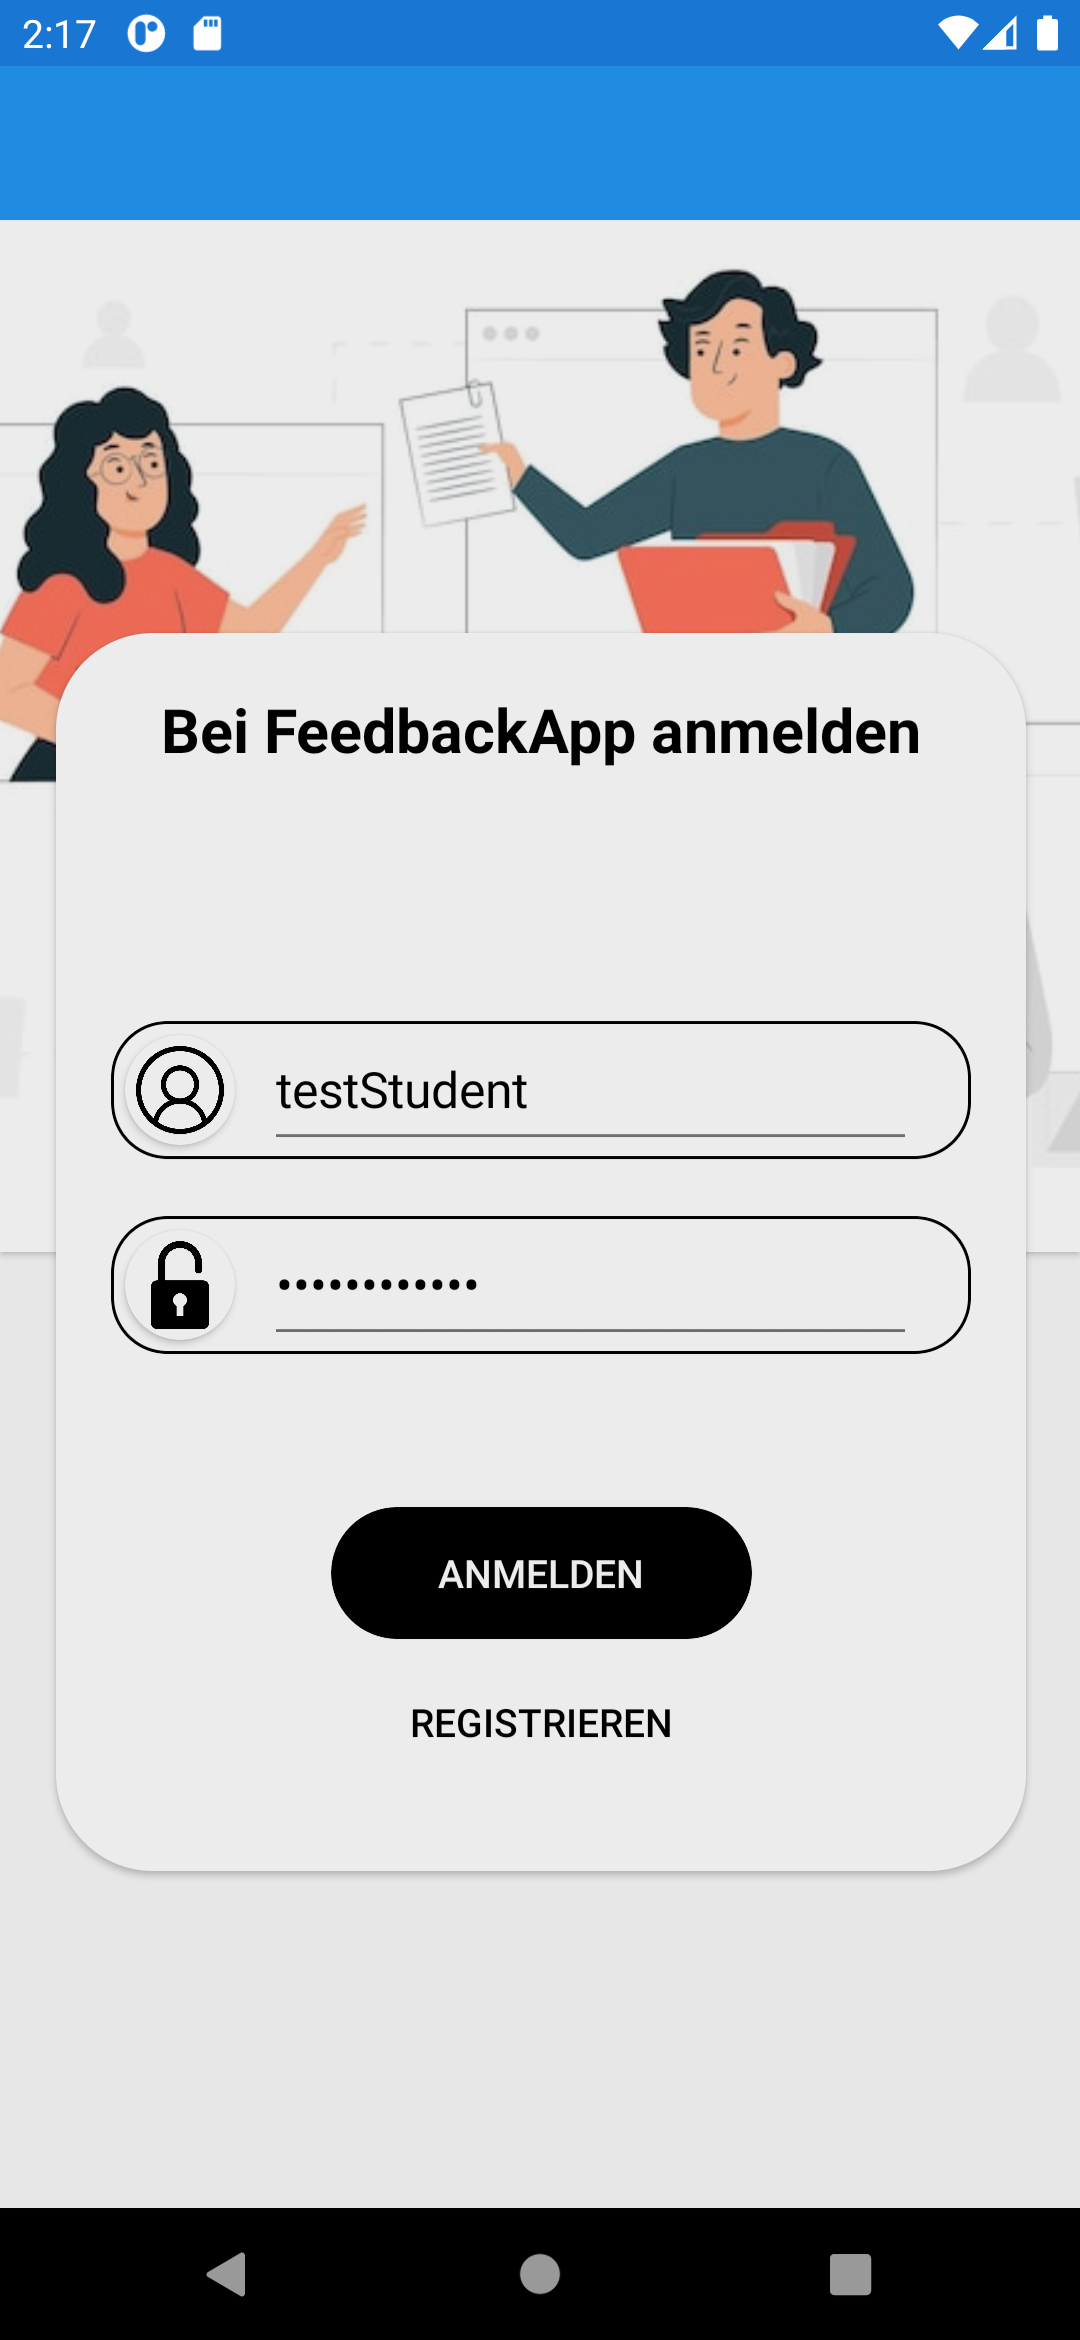
\includegraphics[width=5cm]{pics/Xamarin Student/5 Login Page Full.png}\hfill
    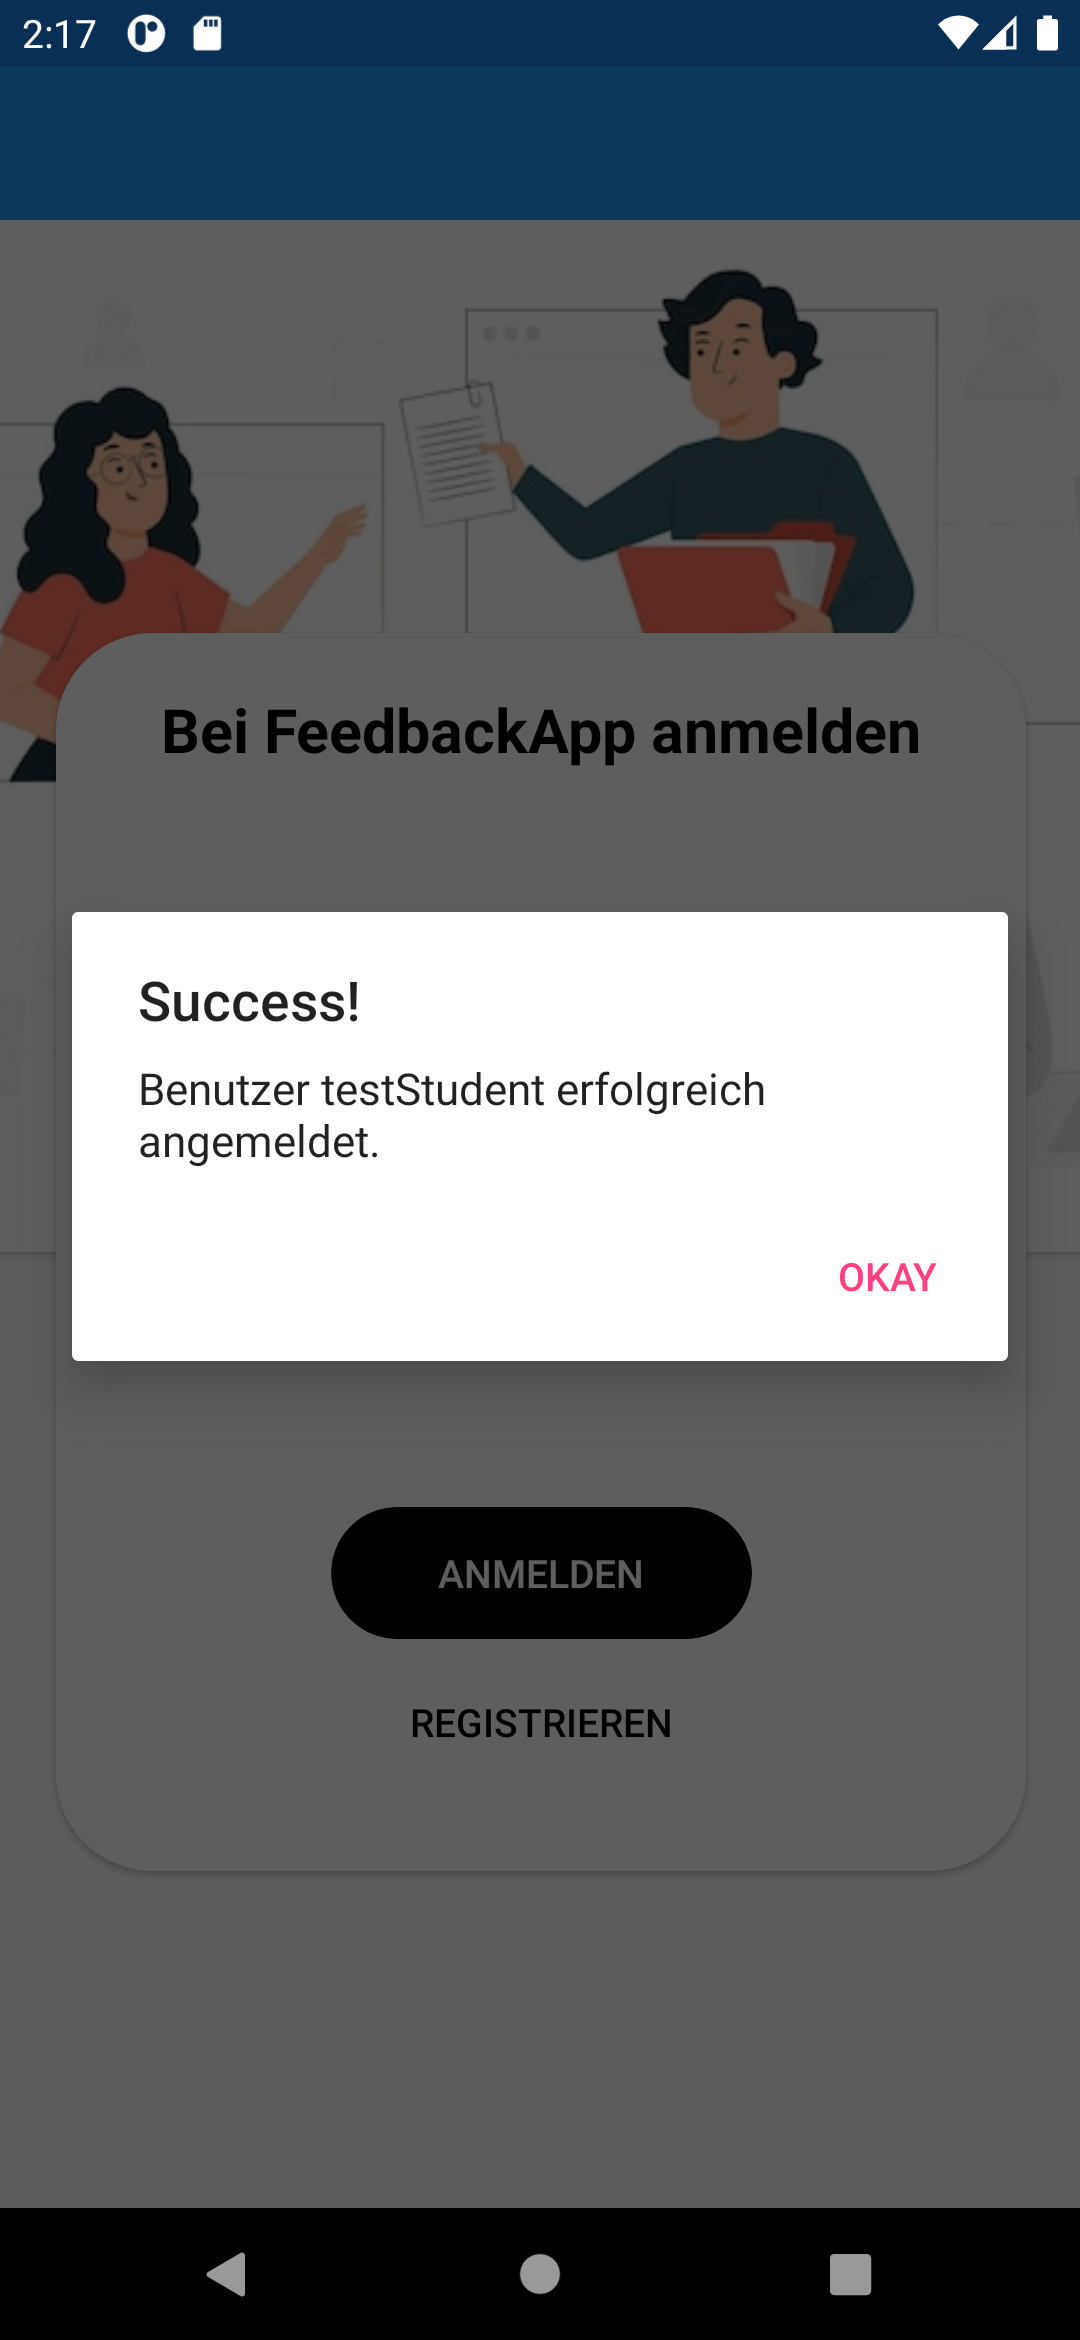
\includegraphics[width=5cm]{pics/Xamarin Student/6 Login Page Success.png}
    \caption[LoginPage Ansicht]{Login Daten einfügen}
    \end{center}
\end{figure}
Durch die Eingabe von Benutzername und Passwort prüfen wir, ob bereits ein Account eingerichtet ist. Wenn das Konto bereits existiert, erhalten wir eine positive Antwort, andernfalls erhalten wir einen Fehler ("error"). Die Anmeldung ist für Schüler und Lehrer gleich, daher gibt es nur eine Anmeldeschaltfläche für alle Benutzer.\newpage
\newpage

\section{Startseite}
\subsection{Schüler}
Die Startseite für Studierende ist einfach gehalten mit der Hauptfunktion der Fächersuche (Feedbackname). Ganz unten befindet sich ein Button "Feedback geben", der nur aktiviert wird, wenn "Einheit" gefunden wird. In der oberen rechten Ecke befindet sich eine Schaltfläche, die zu den persönlichen Daten des Benutzers führt, wo die Daten angepasst, geändert oder gelöscht werden können. In der Mitte der Seite befindet sich eine Suchmaschine für alle Fächer (Einheit), und der Name muss genau eingegeben werden, um die richtigen Ergebnisse zurückzugeben.
\begin{figure}[h]
    \begin{center}
        \includegraphics*[width=5cm]{pics/Xamarin Student/7 HomePage Student.png}
        \caption[HomePage Student Ansicht]{HomePage Student Ansicht}
    \end{center}
\end{figure}
\newpage
Zunächst muss der richtige Name des Themas oder zumindest der richtige Anfangsteil eingegeben werden, und nach der Suchmaschine erhalten wir korrekte Ergebnisse.
\begin{figure}[h]
    \begin{center}
    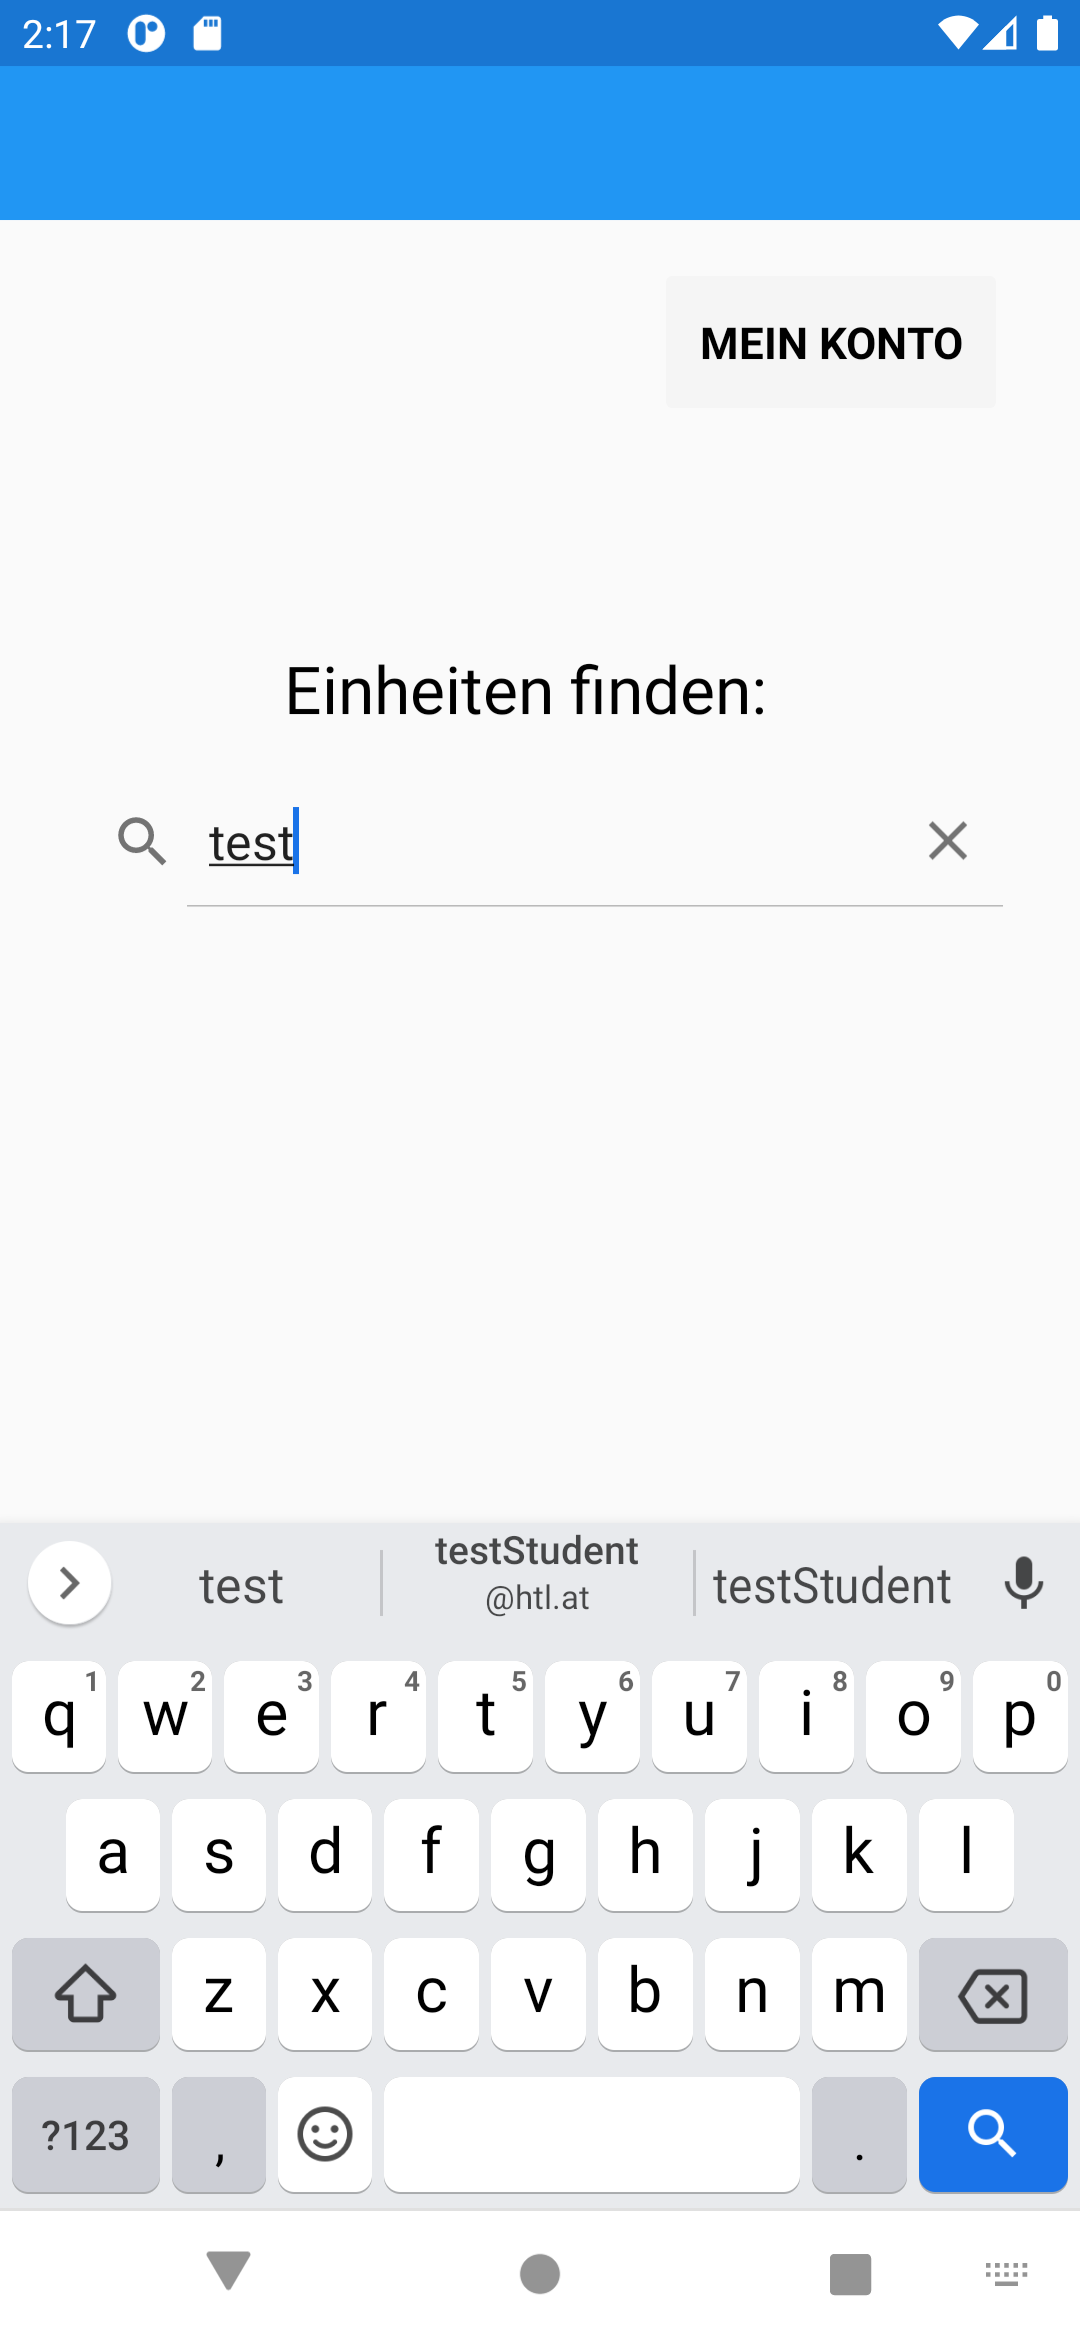
\includegraphics[width=4cm]{pics/Xamarin Student/8 Einheit finden.png}\hfill
    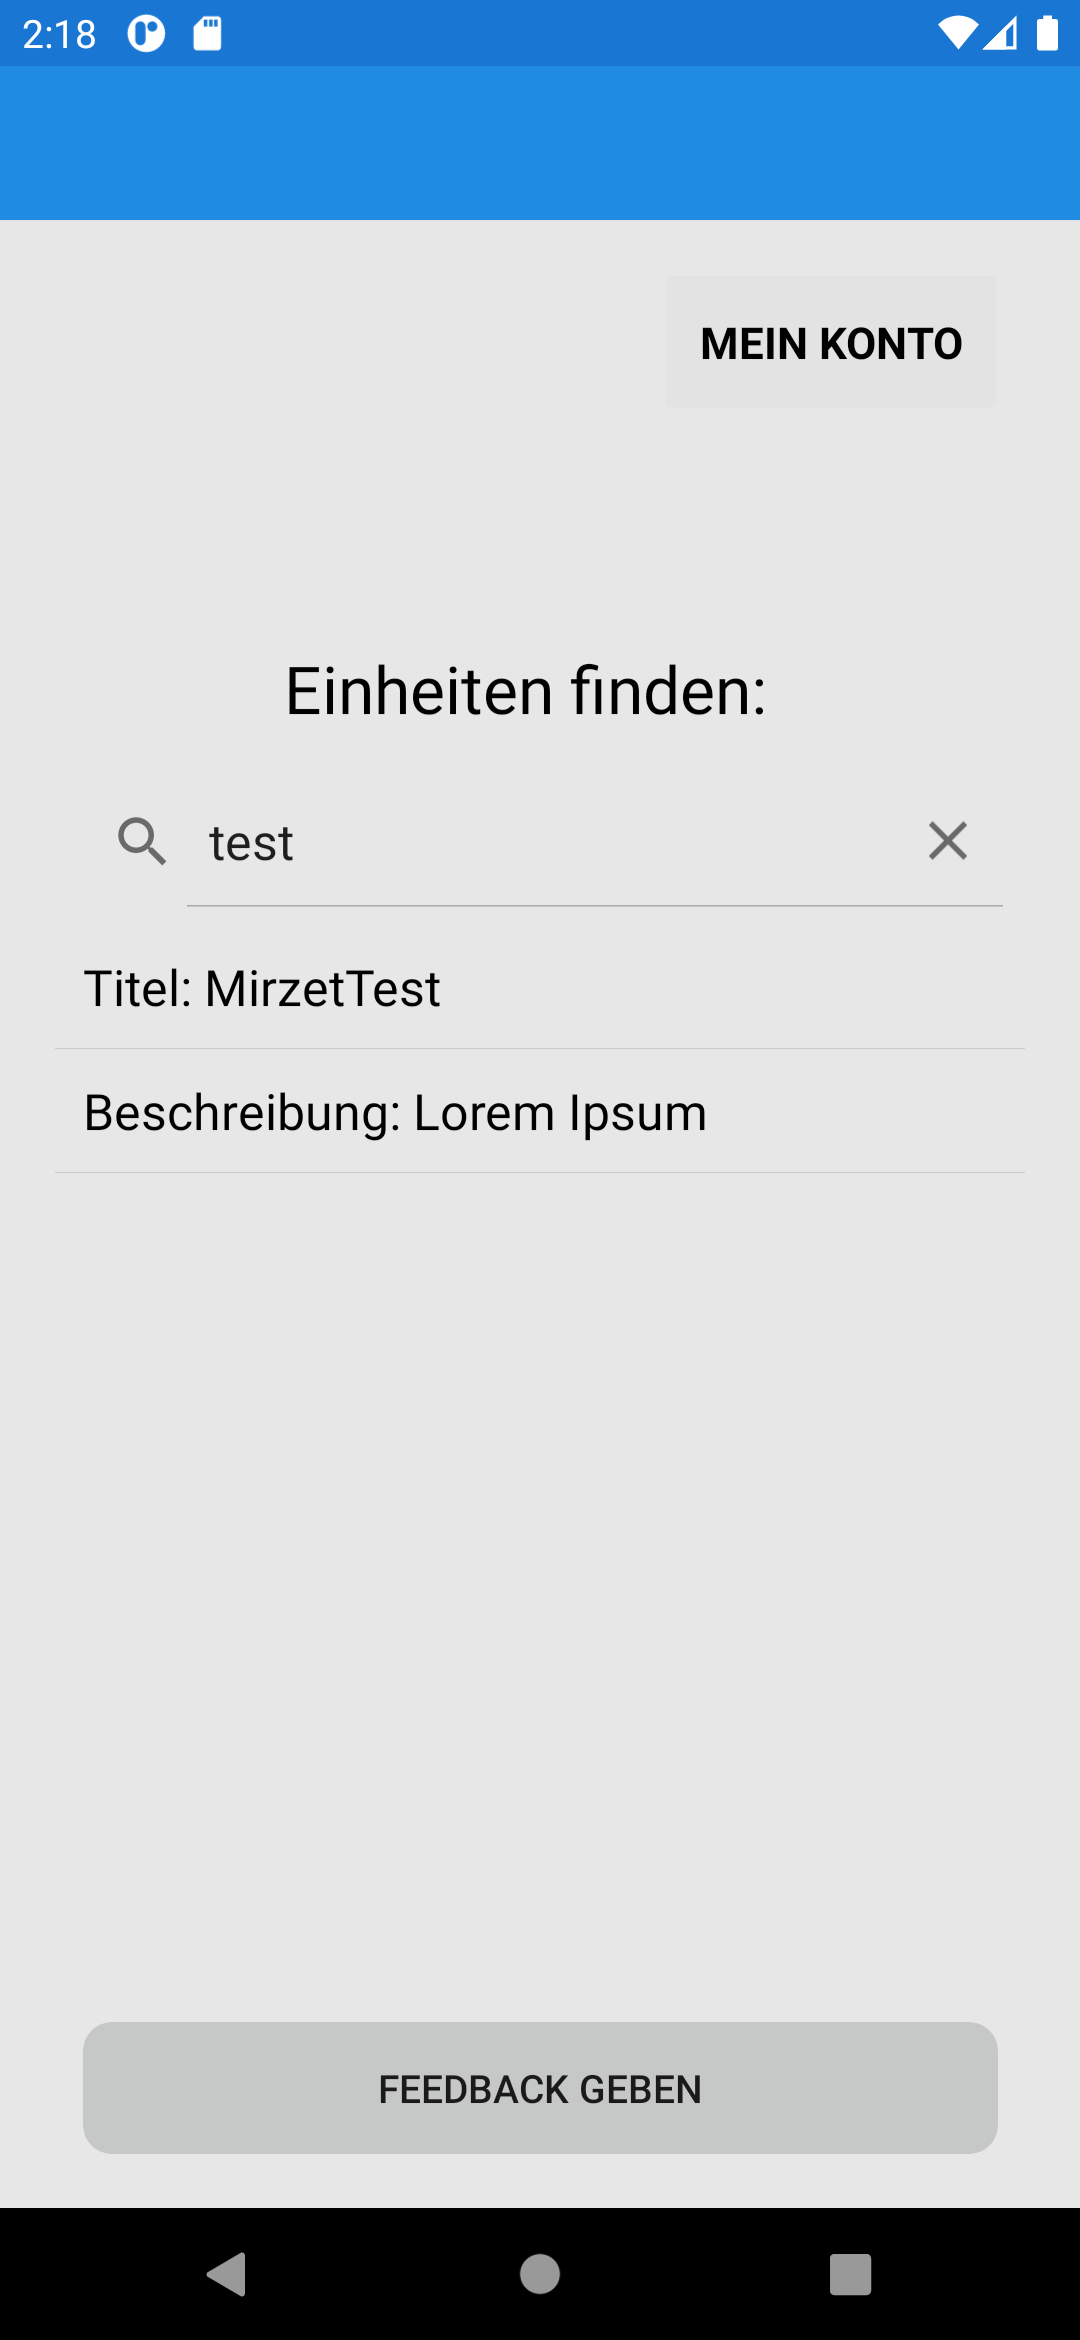
\includegraphics[width=4cm]{pics/Xamarin Student/9 Einheit gefunden.png}
    \caption[HomePage Einheiten Ansicht]{Einheiten Ansicht}
    \end{center}
\end{figure}
\newpage

Nachdem der Artikel gefunden wurde, wird die Schaltfläche unten auf der Seite sichtbar und aktiv, und wir können darauf klicken, wenn wir Feedback oder einen Kommentar hinterlassen möchten.
\begin{figure}[h]
    \begin{center}
    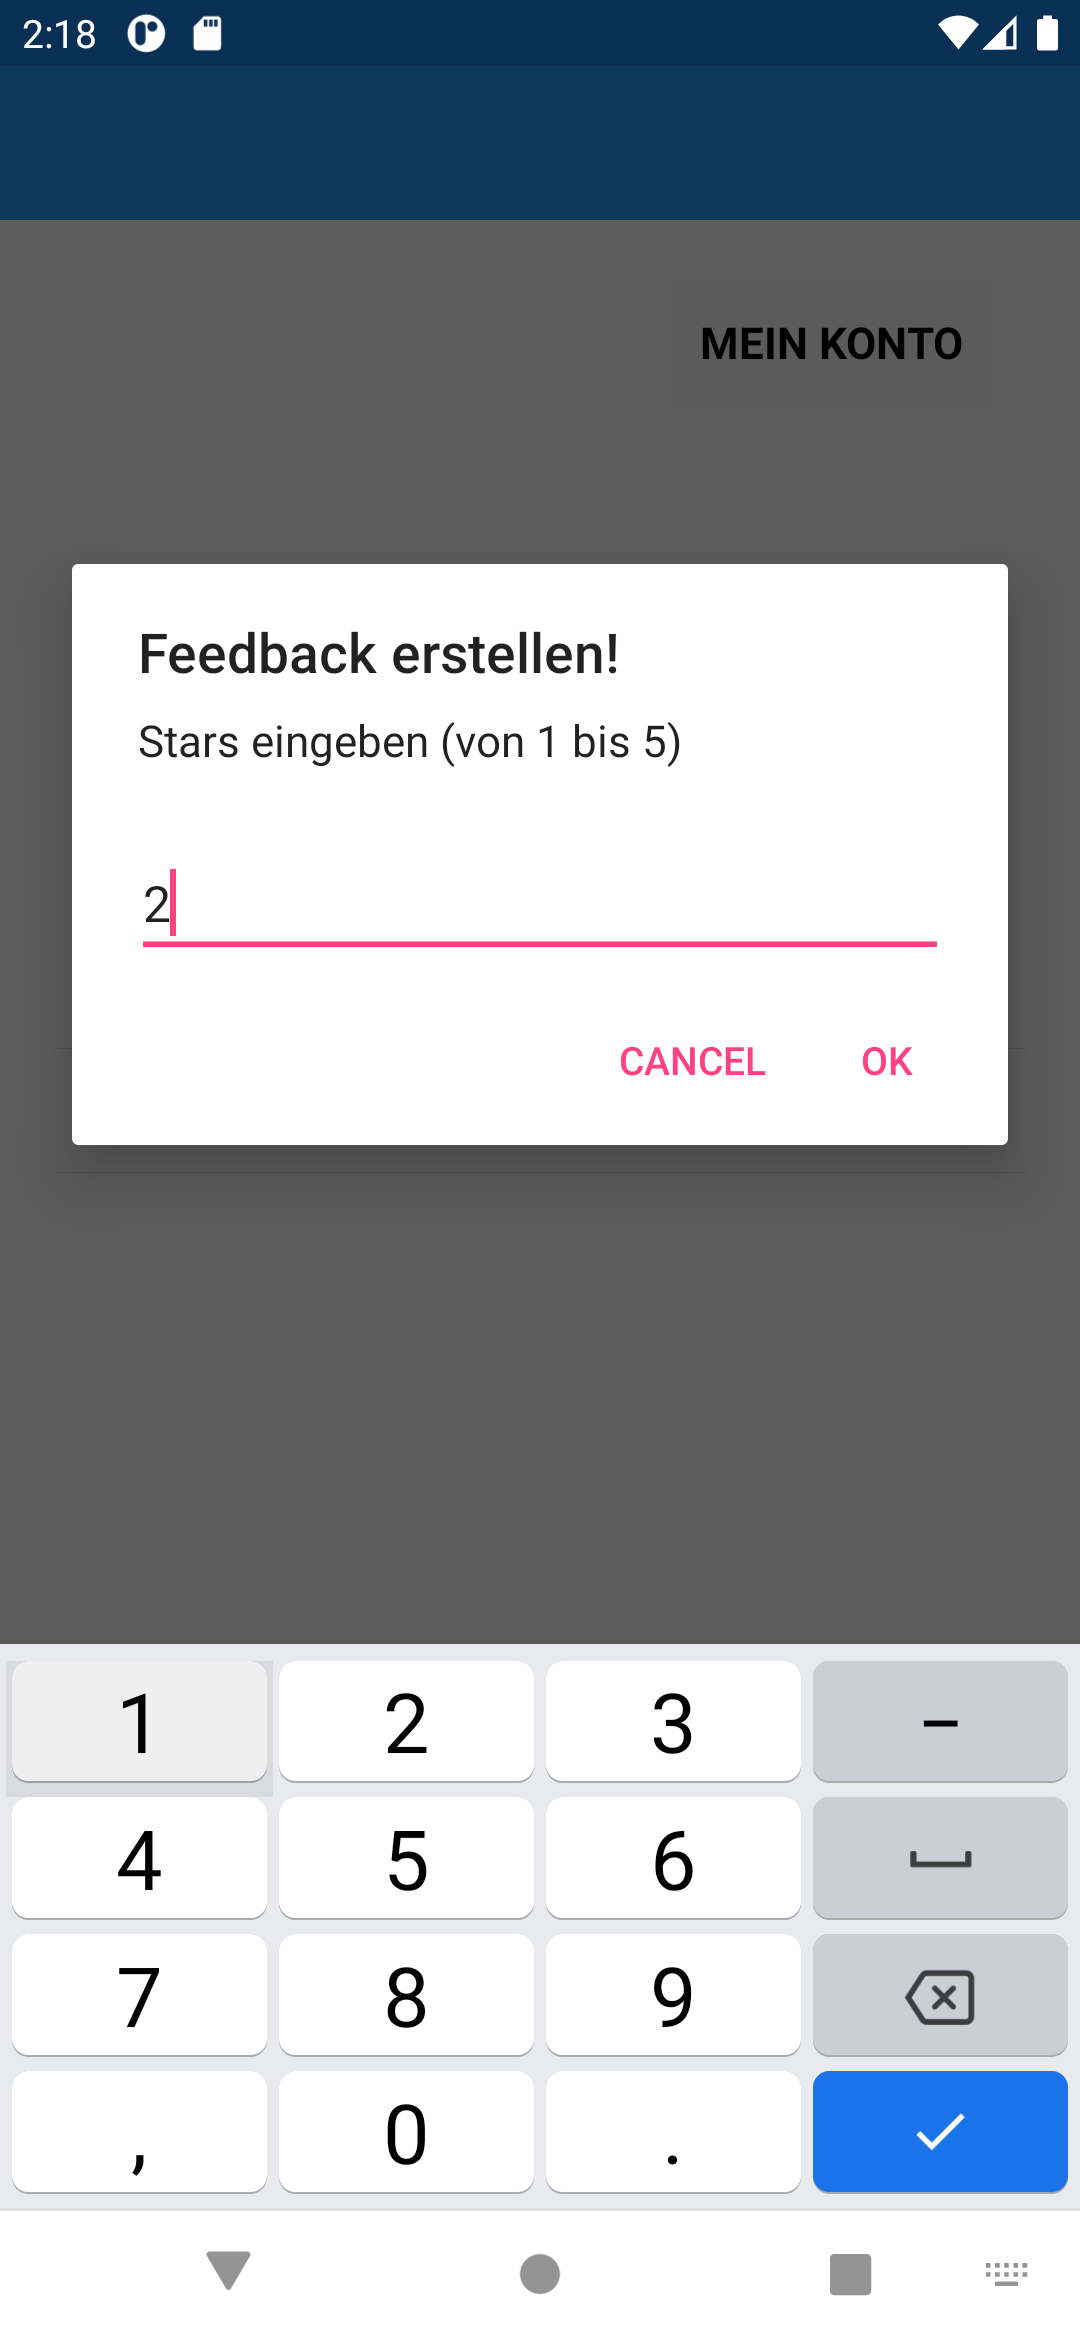
\includegraphics[width=4cm]{pics/Xamarin Student/10 Feedback Star.png}\hfill
    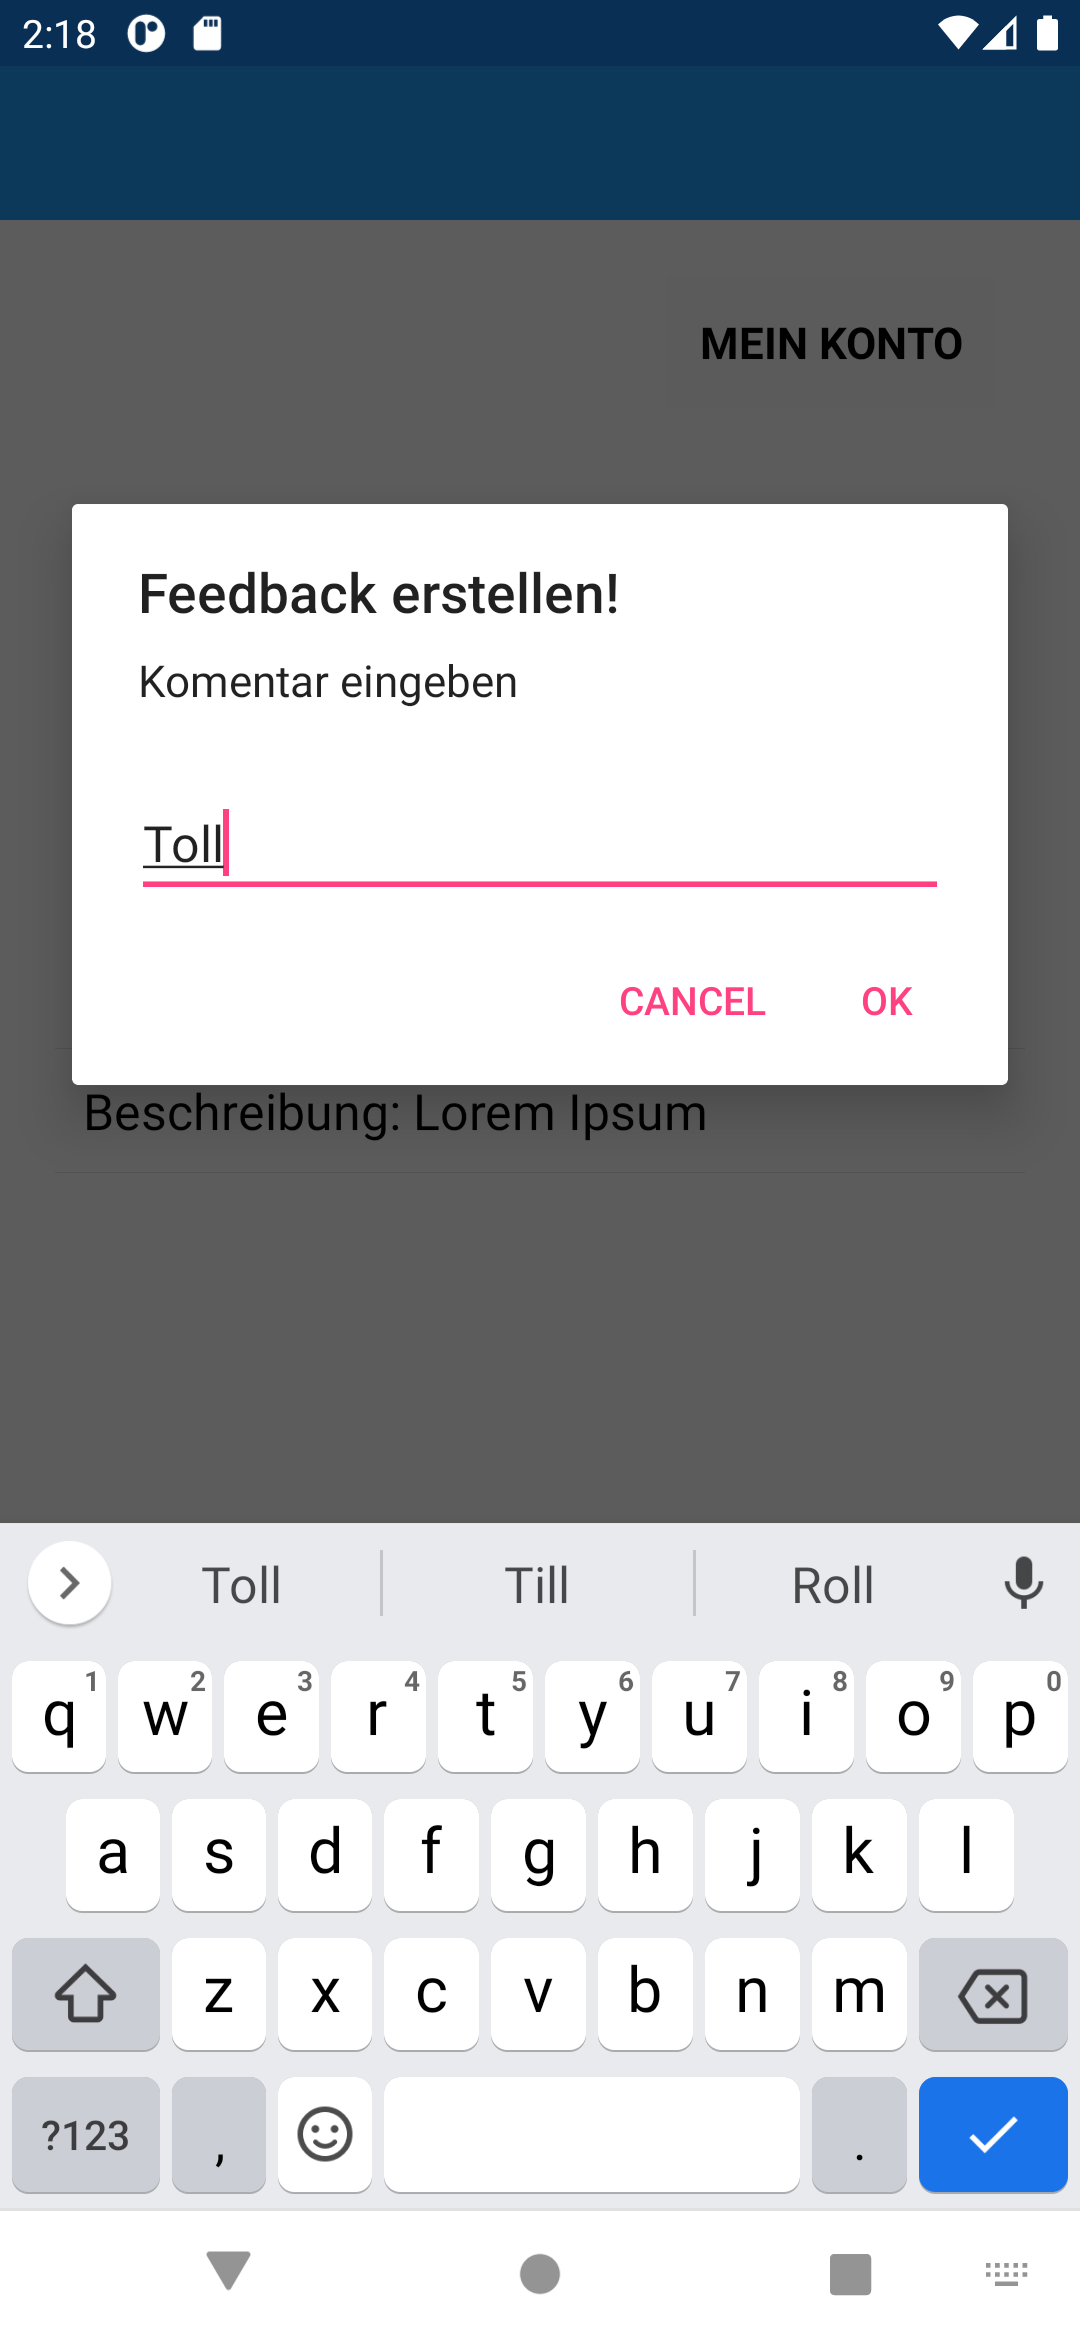
\includegraphics[width=4cm]{pics/Xamarin Student/11 Feedback comm.png}\hfill
    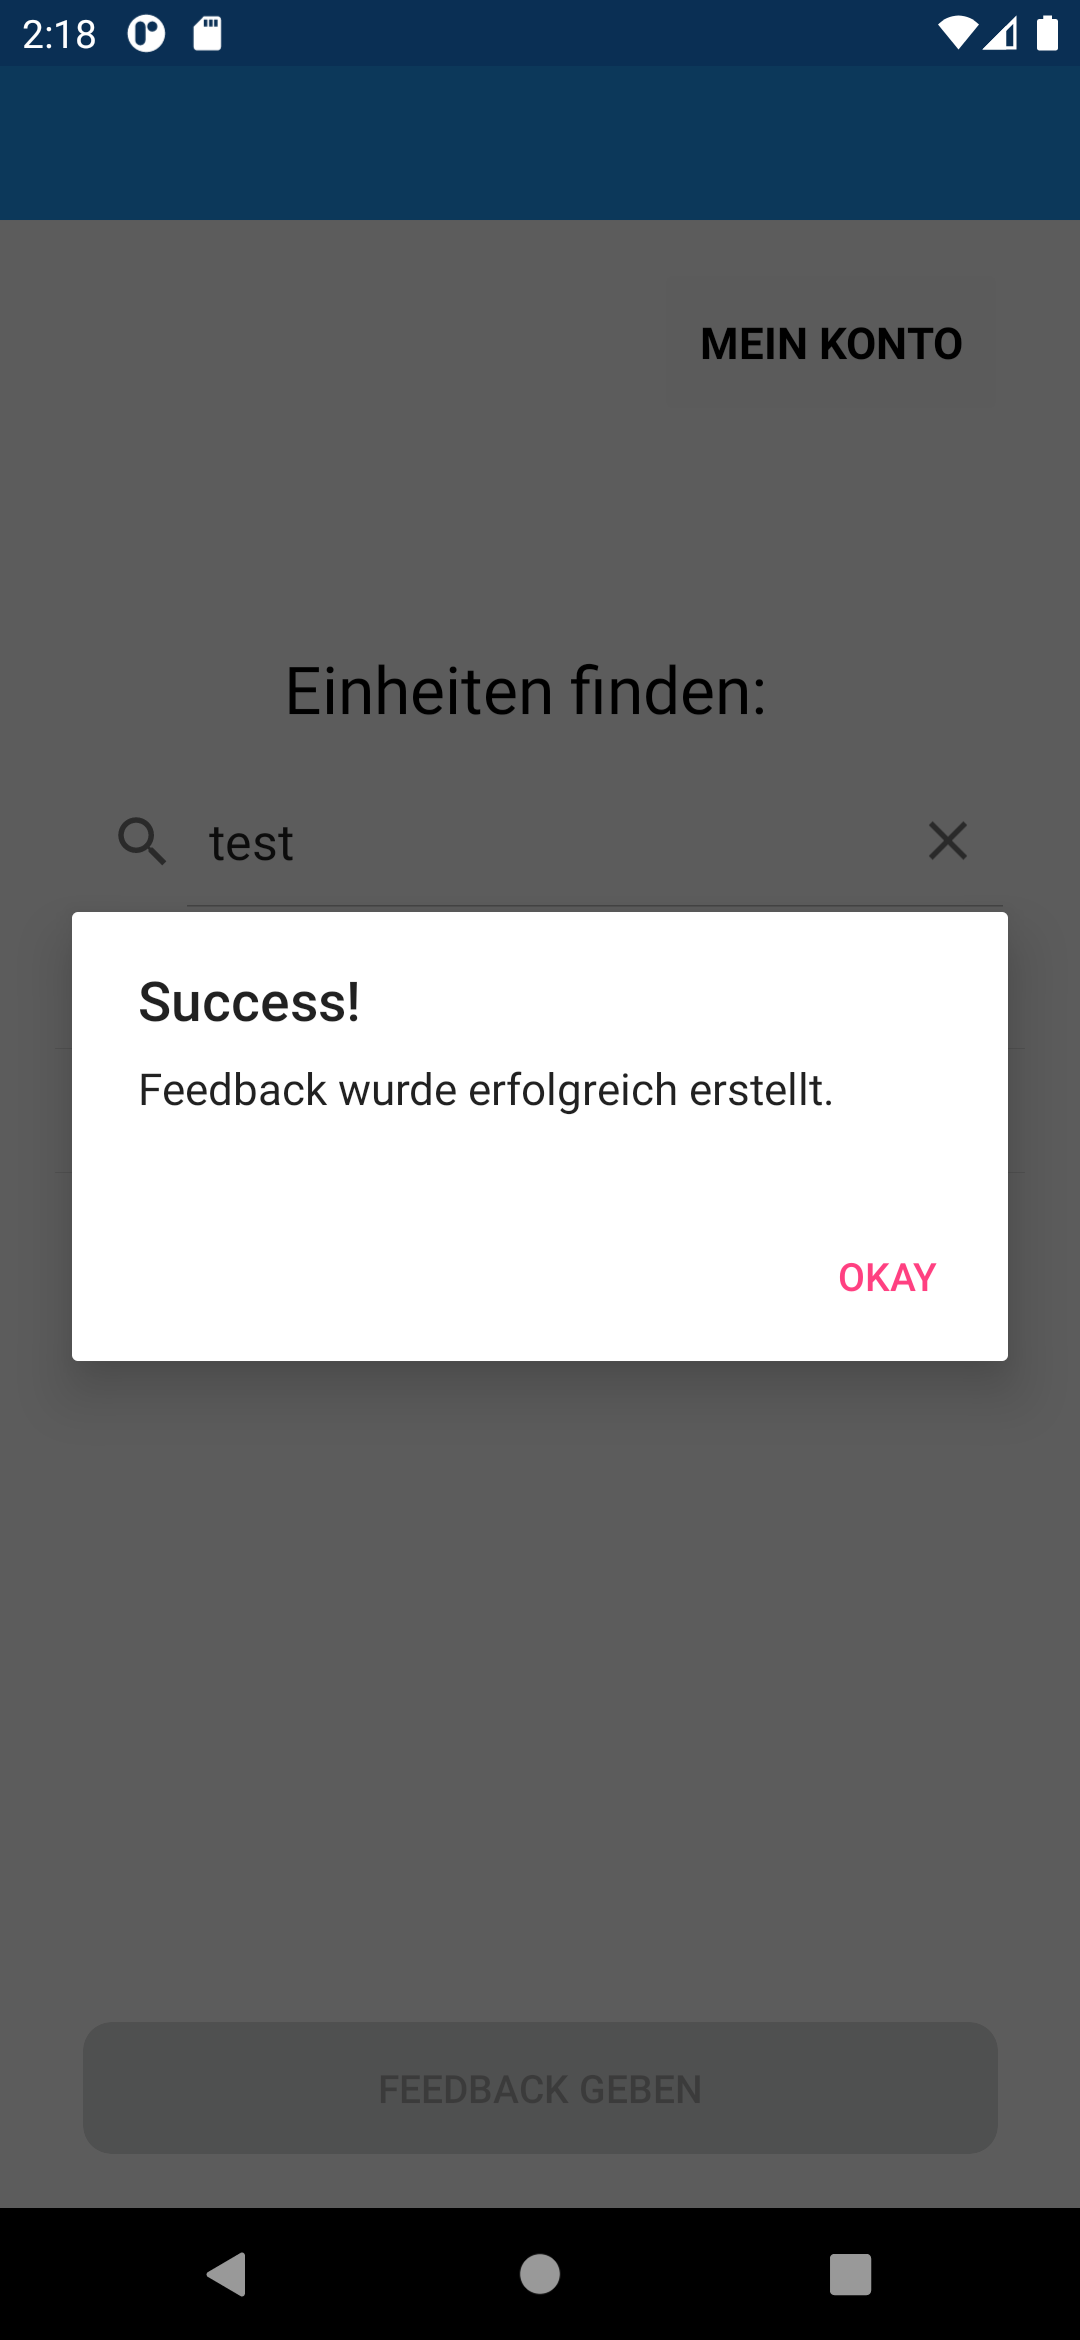
\includegraphics[width=4cm]{pics/Xamarin Student/12 Feedback success.png}
    \caption[HomePage Feedback geben]{Feedback geben Ansicht}
    \end{center}
\end{figure}
\newline
Wenn wir eine Bewertung über 5 oder unter 1 eingeben, erhalten wir eine Fehlermeldung und das Feedback wird nicht gespeichert.
Nach erfolgreicher Abgabe von Feedback ist der Button „Feedback geben“ wieder inaktiv und wir können es nicht noch einmal geben.
\newpage

\subsection{Lehrer}
Die Startseite für Lehrer ist die gleiche wie für Schüler, nur haben wir zusätzlich einen Button zum Anlegen von Fächern. Darüber hinaus gibt es auch eine Suchmaschine, um zu prüfen, ob der Artikel, den wir eingeben möchten, bereits existiert. Natürlich gibt es auch einen Button für das Benutzerkonto.
\begin{figure}[h]
    \begin{center}
        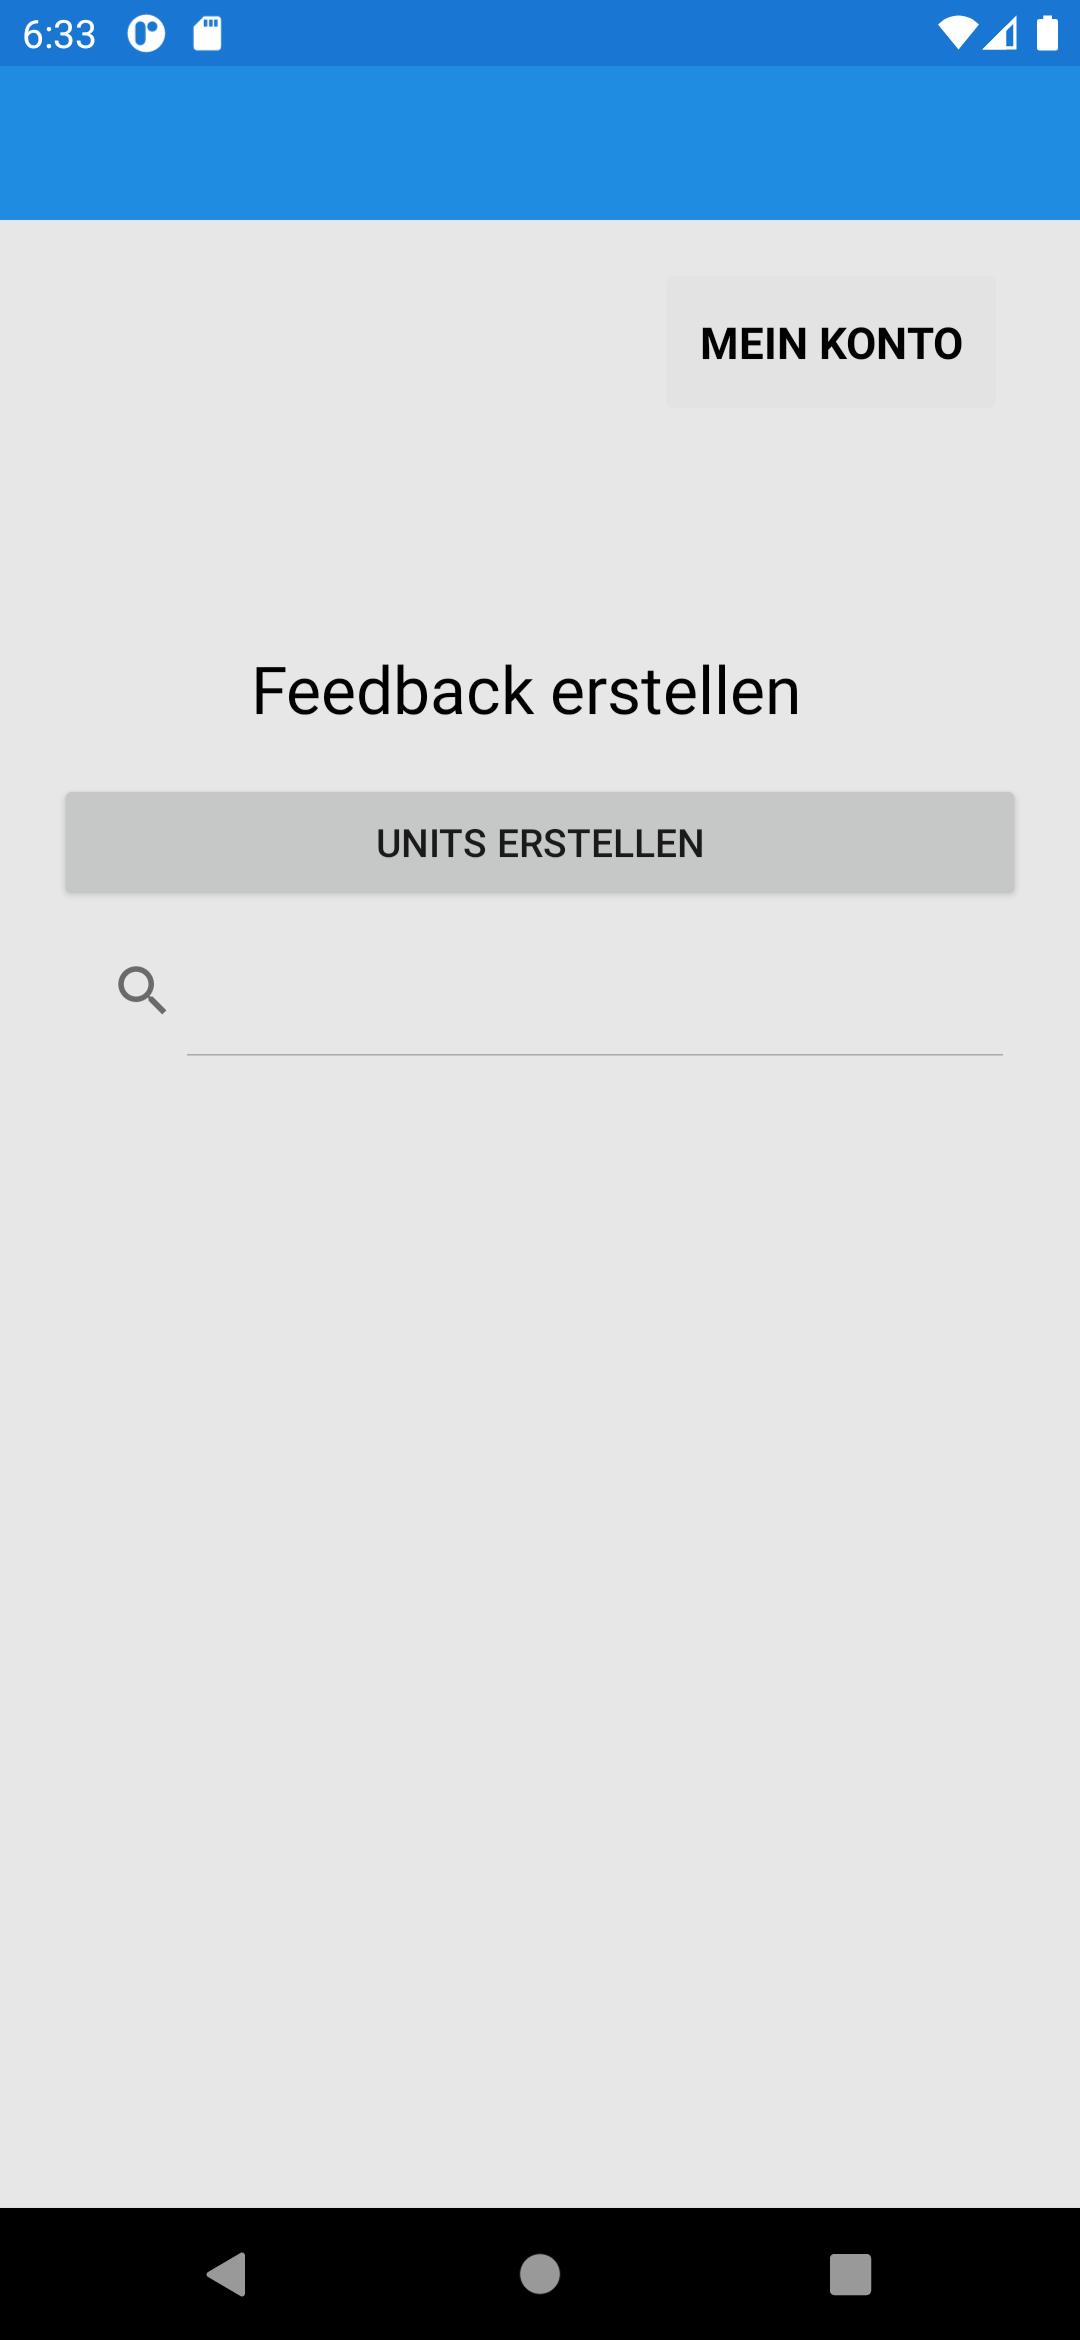
\includegraphics[width=4cm]{pics/Xamarin Lehrer/2 HomePage Lehrer.png}\hfill
        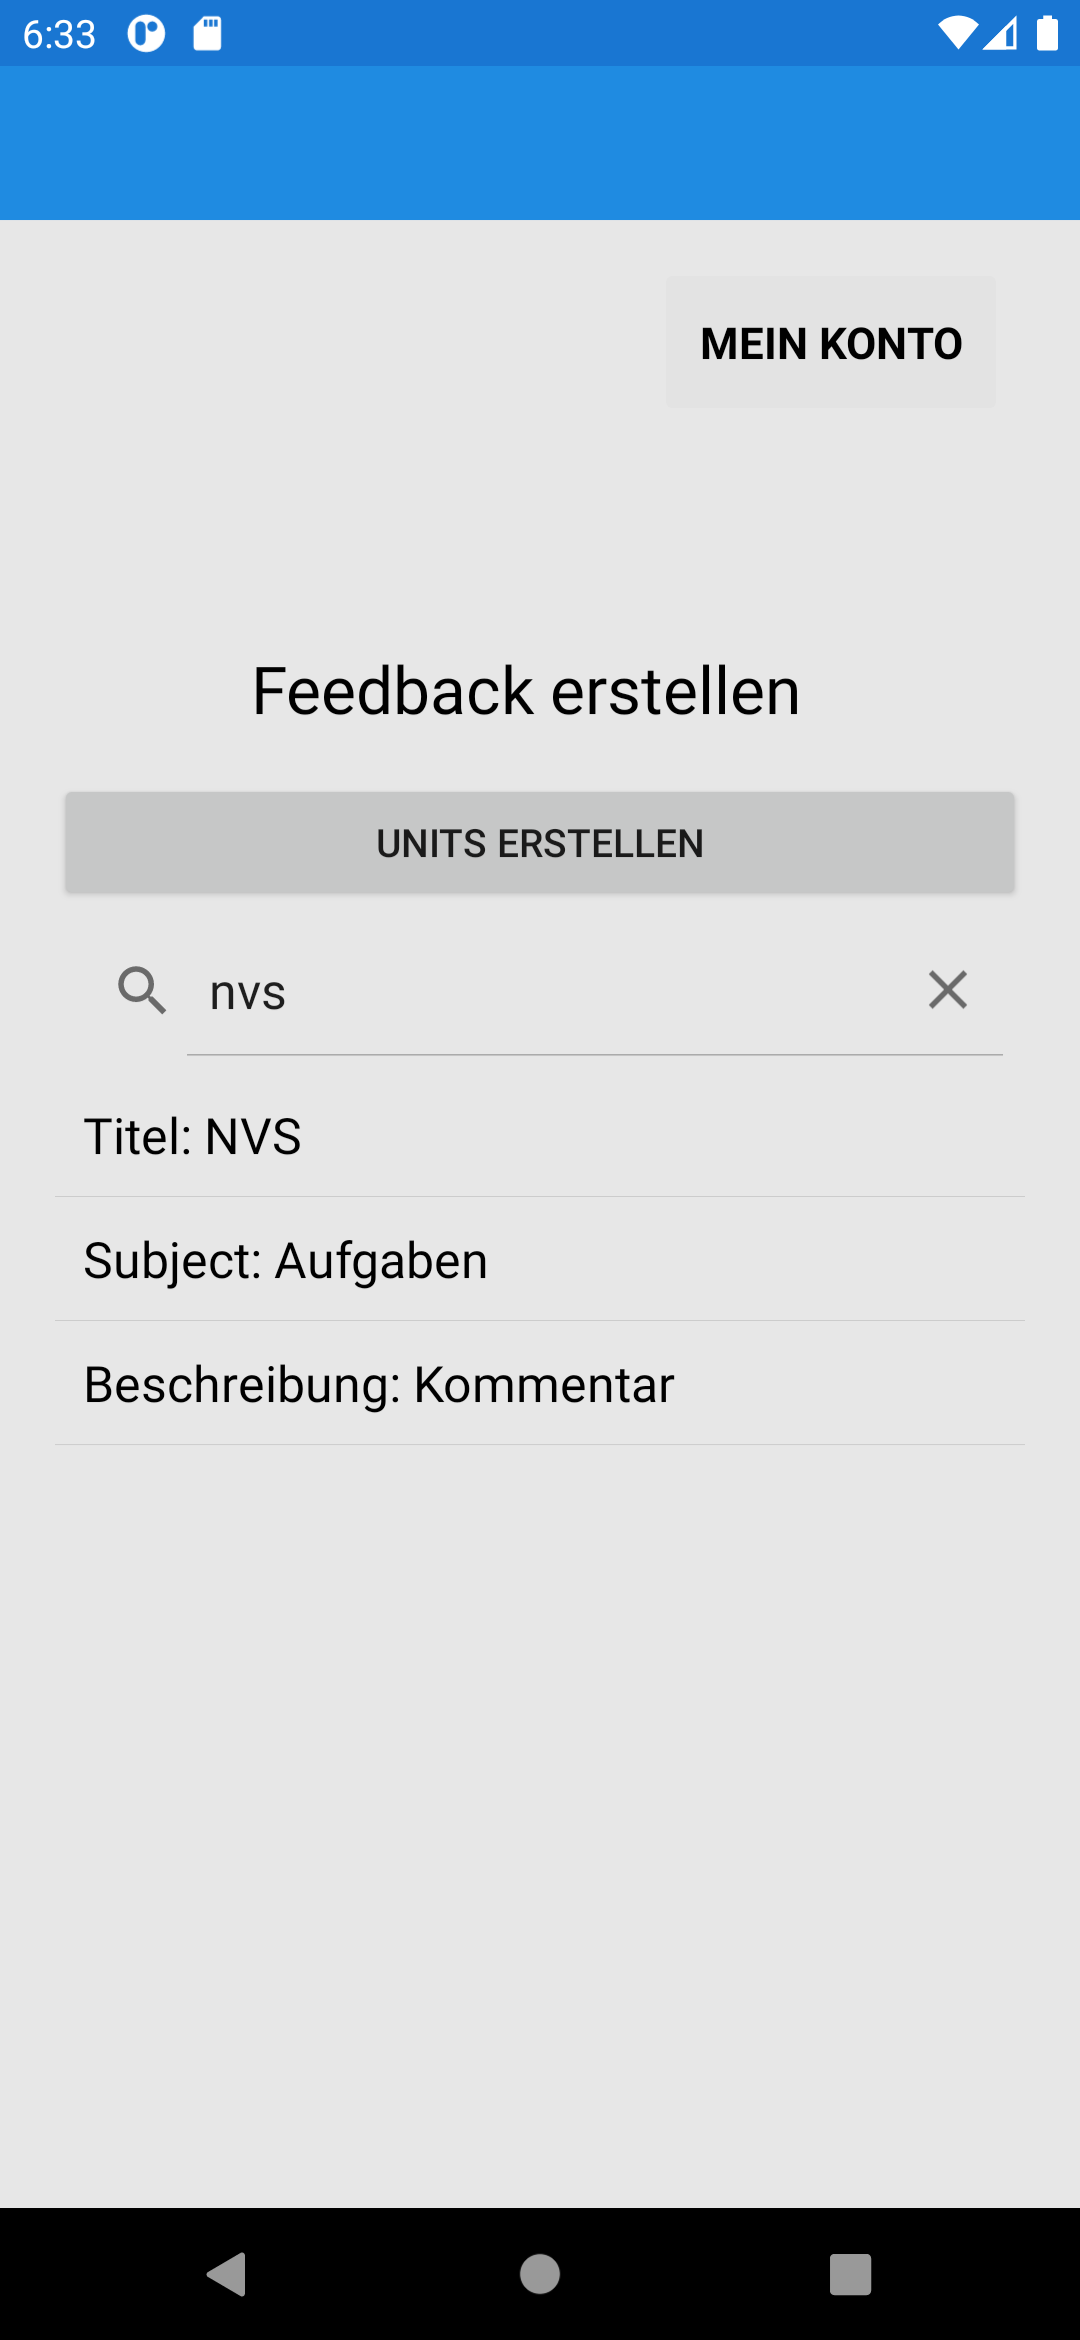
\includegraphics[width=4cm]{pics/Xamarin Lehrer/3 Unit finden.png}
        \caption[HomePage Lehrer Ansicht]{HomePage Lehrer Ansicht}
    \end{center}
\end{figure}
\newpage
Um einen neuen Betreff einzugeben, ist die Eingabe von Titel, Betreff und Beschreibung des Betreffs obligatorisch. Das Formular wird in 3 Schritten ausgefüllt, und wenn alles korrekt eingetragen ist, erhalten wir eine positive Antwort.
\begin{figure}[h]
    \begin{center}
        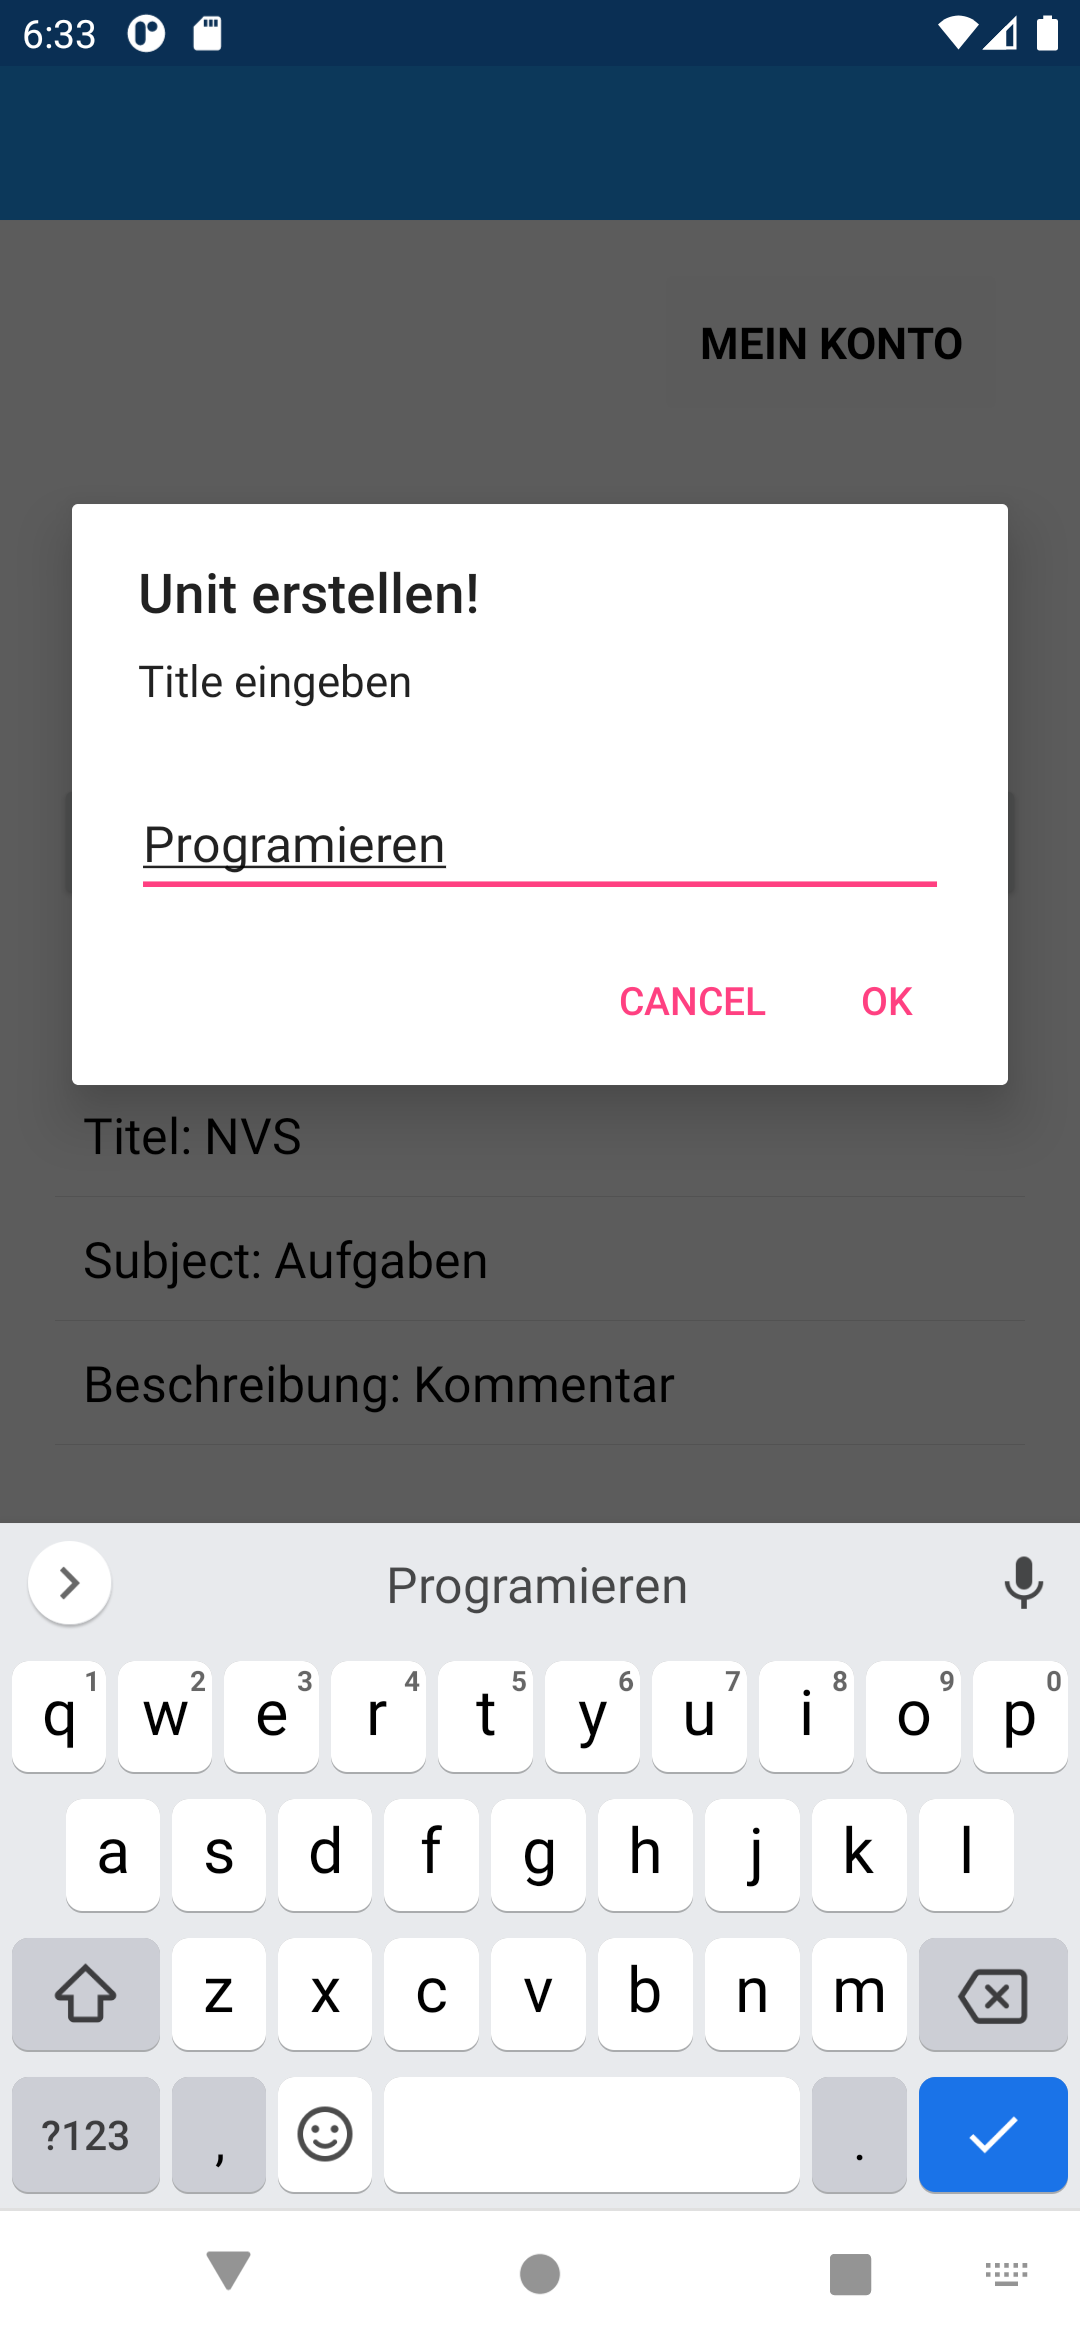
\includegraphics[width=4cm]{pics/Xamarin Lehrer/5.png}\hfill
        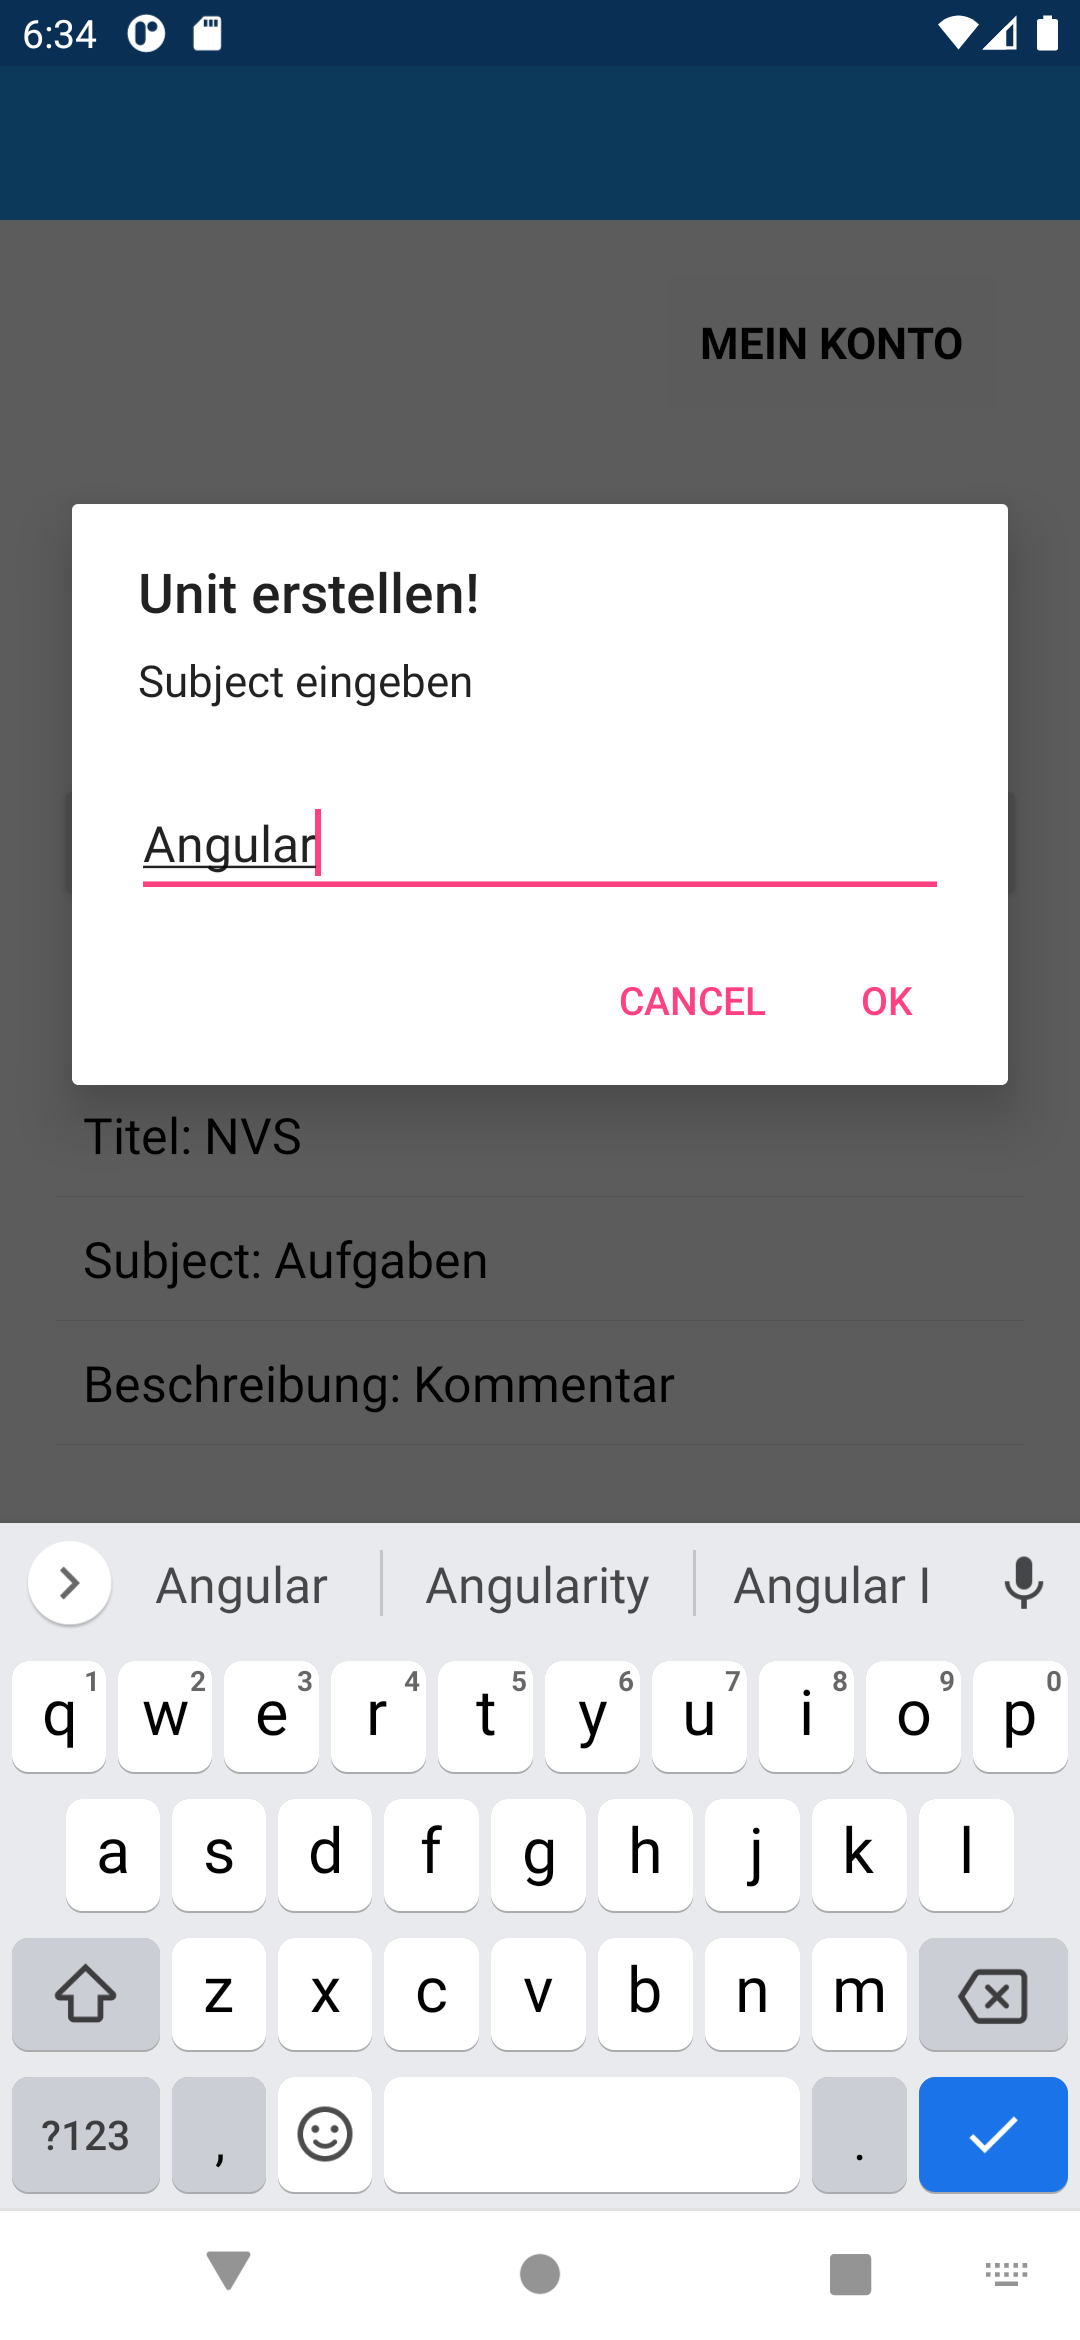
\includegraphics[width=4cm]{pics/Xamarin Lehrer/6.png}
    \end{center}
\end{figure}
\begin{figure}[h]
    \begin{center}
        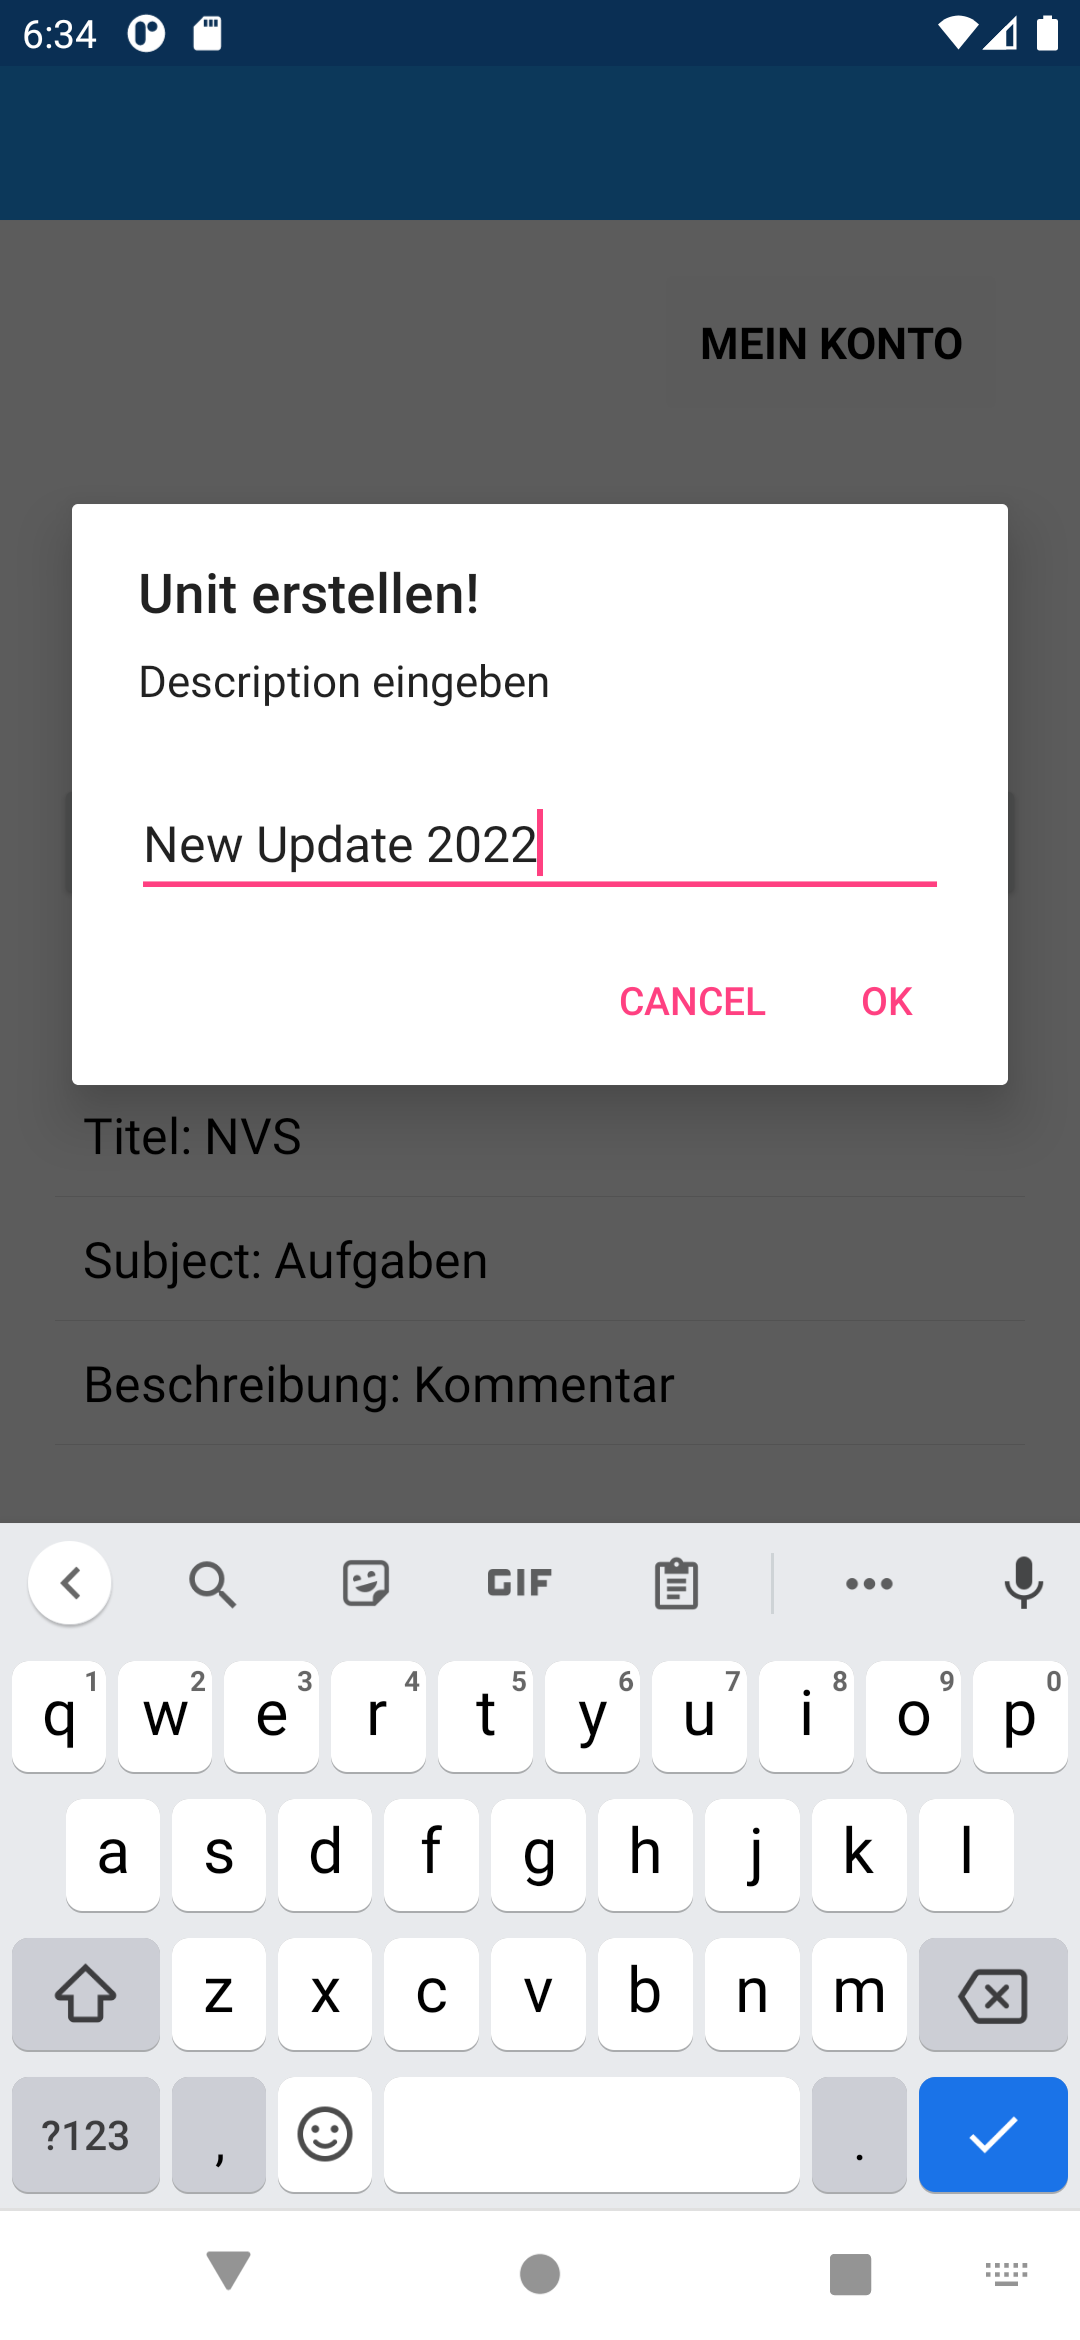
\includegraphics[width=4cm]{pics/Xamarin Lehrer/7.png}\hfill
        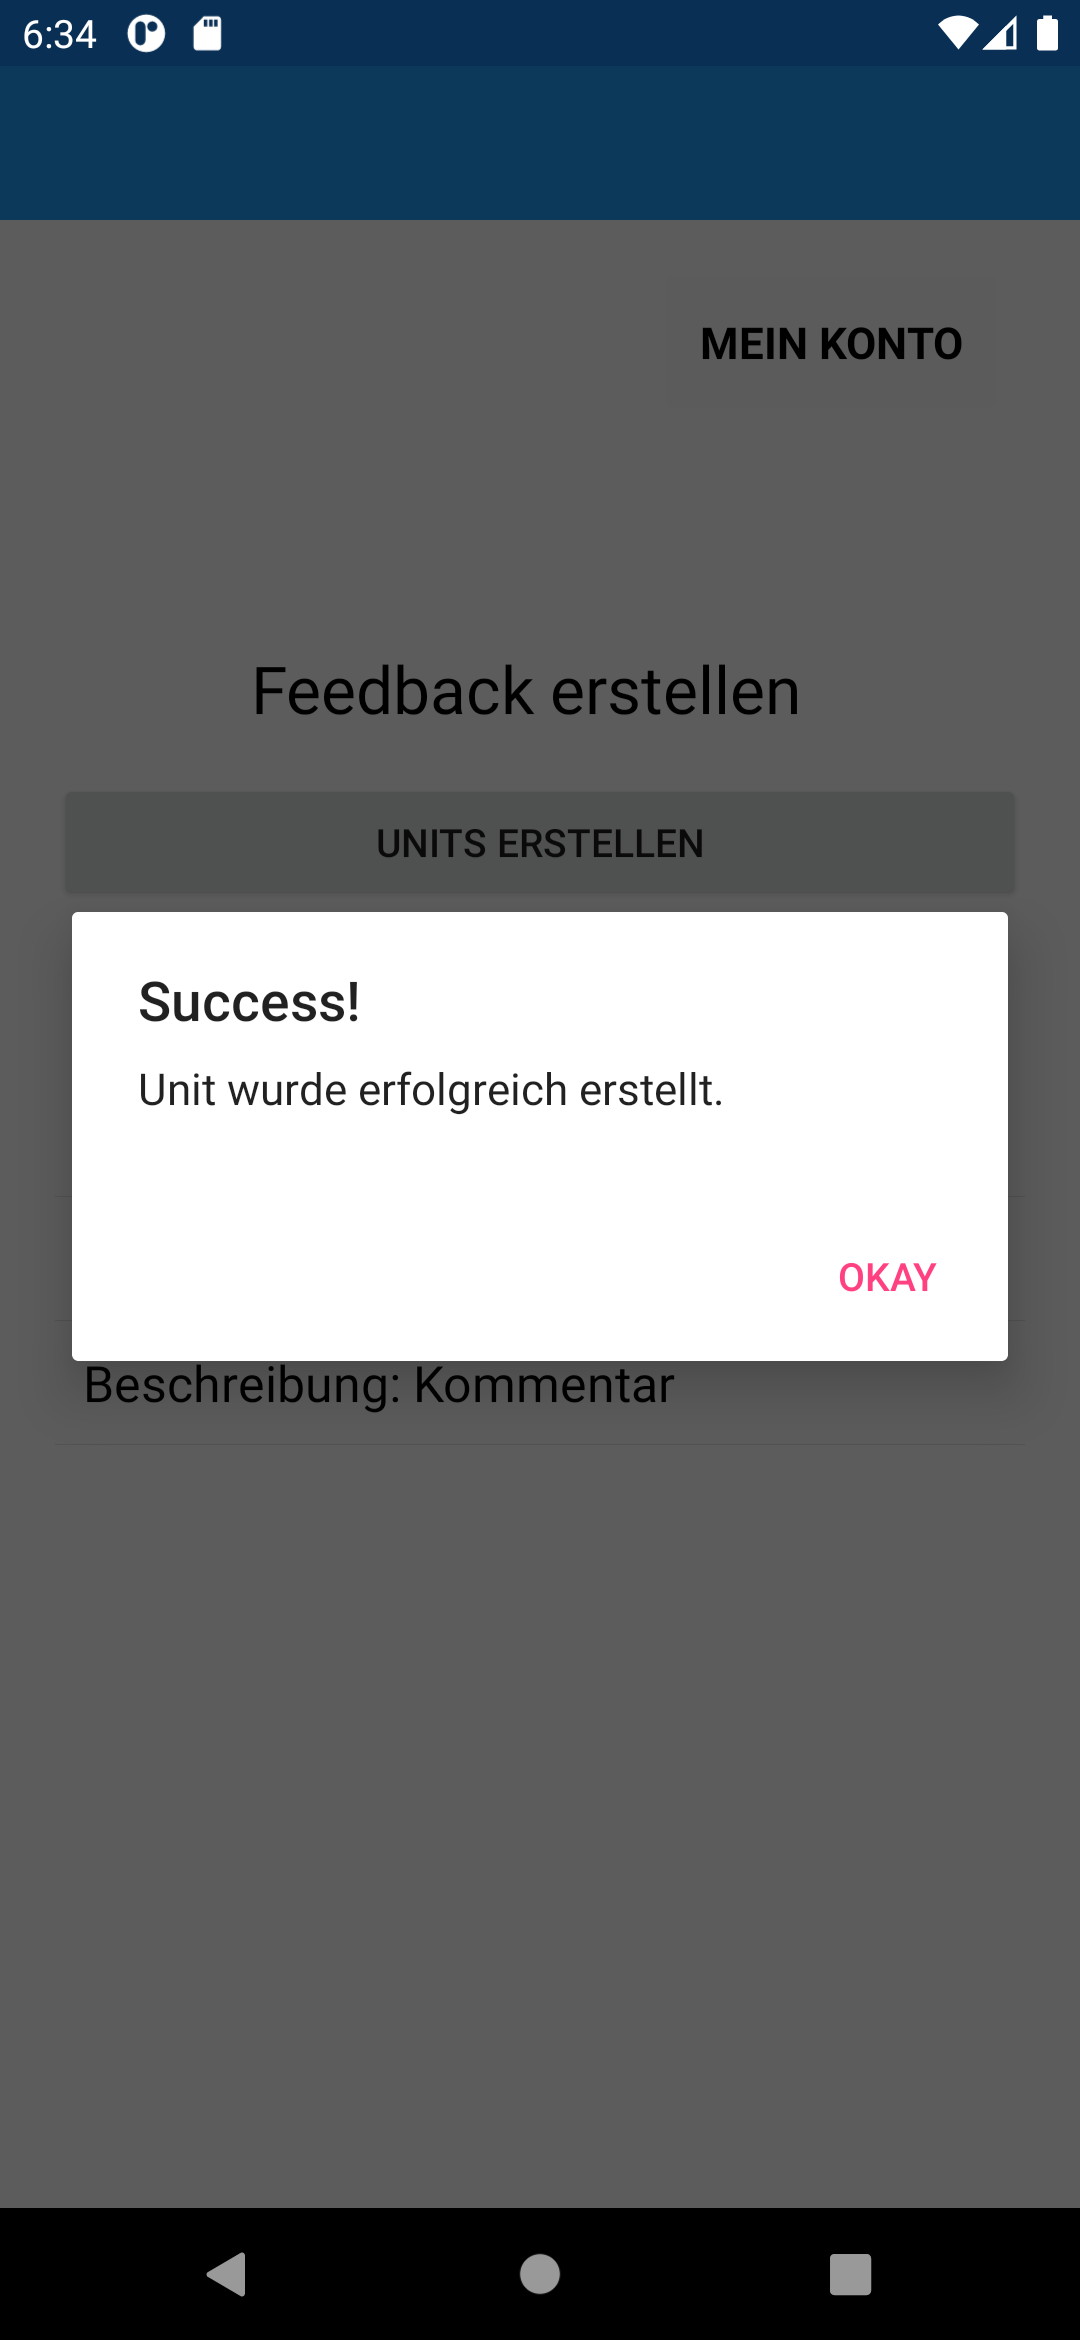
\includegraphics[width=4cm]{pics/Xamarin Lehrer/8.png}
        \caption[HomePage Unit Ansicht]{Unit erstellen}
    \end{center}
\end{figure}
\newpage

\section{Registrierung}
\begin{figure}[h]
    \begin{center}
        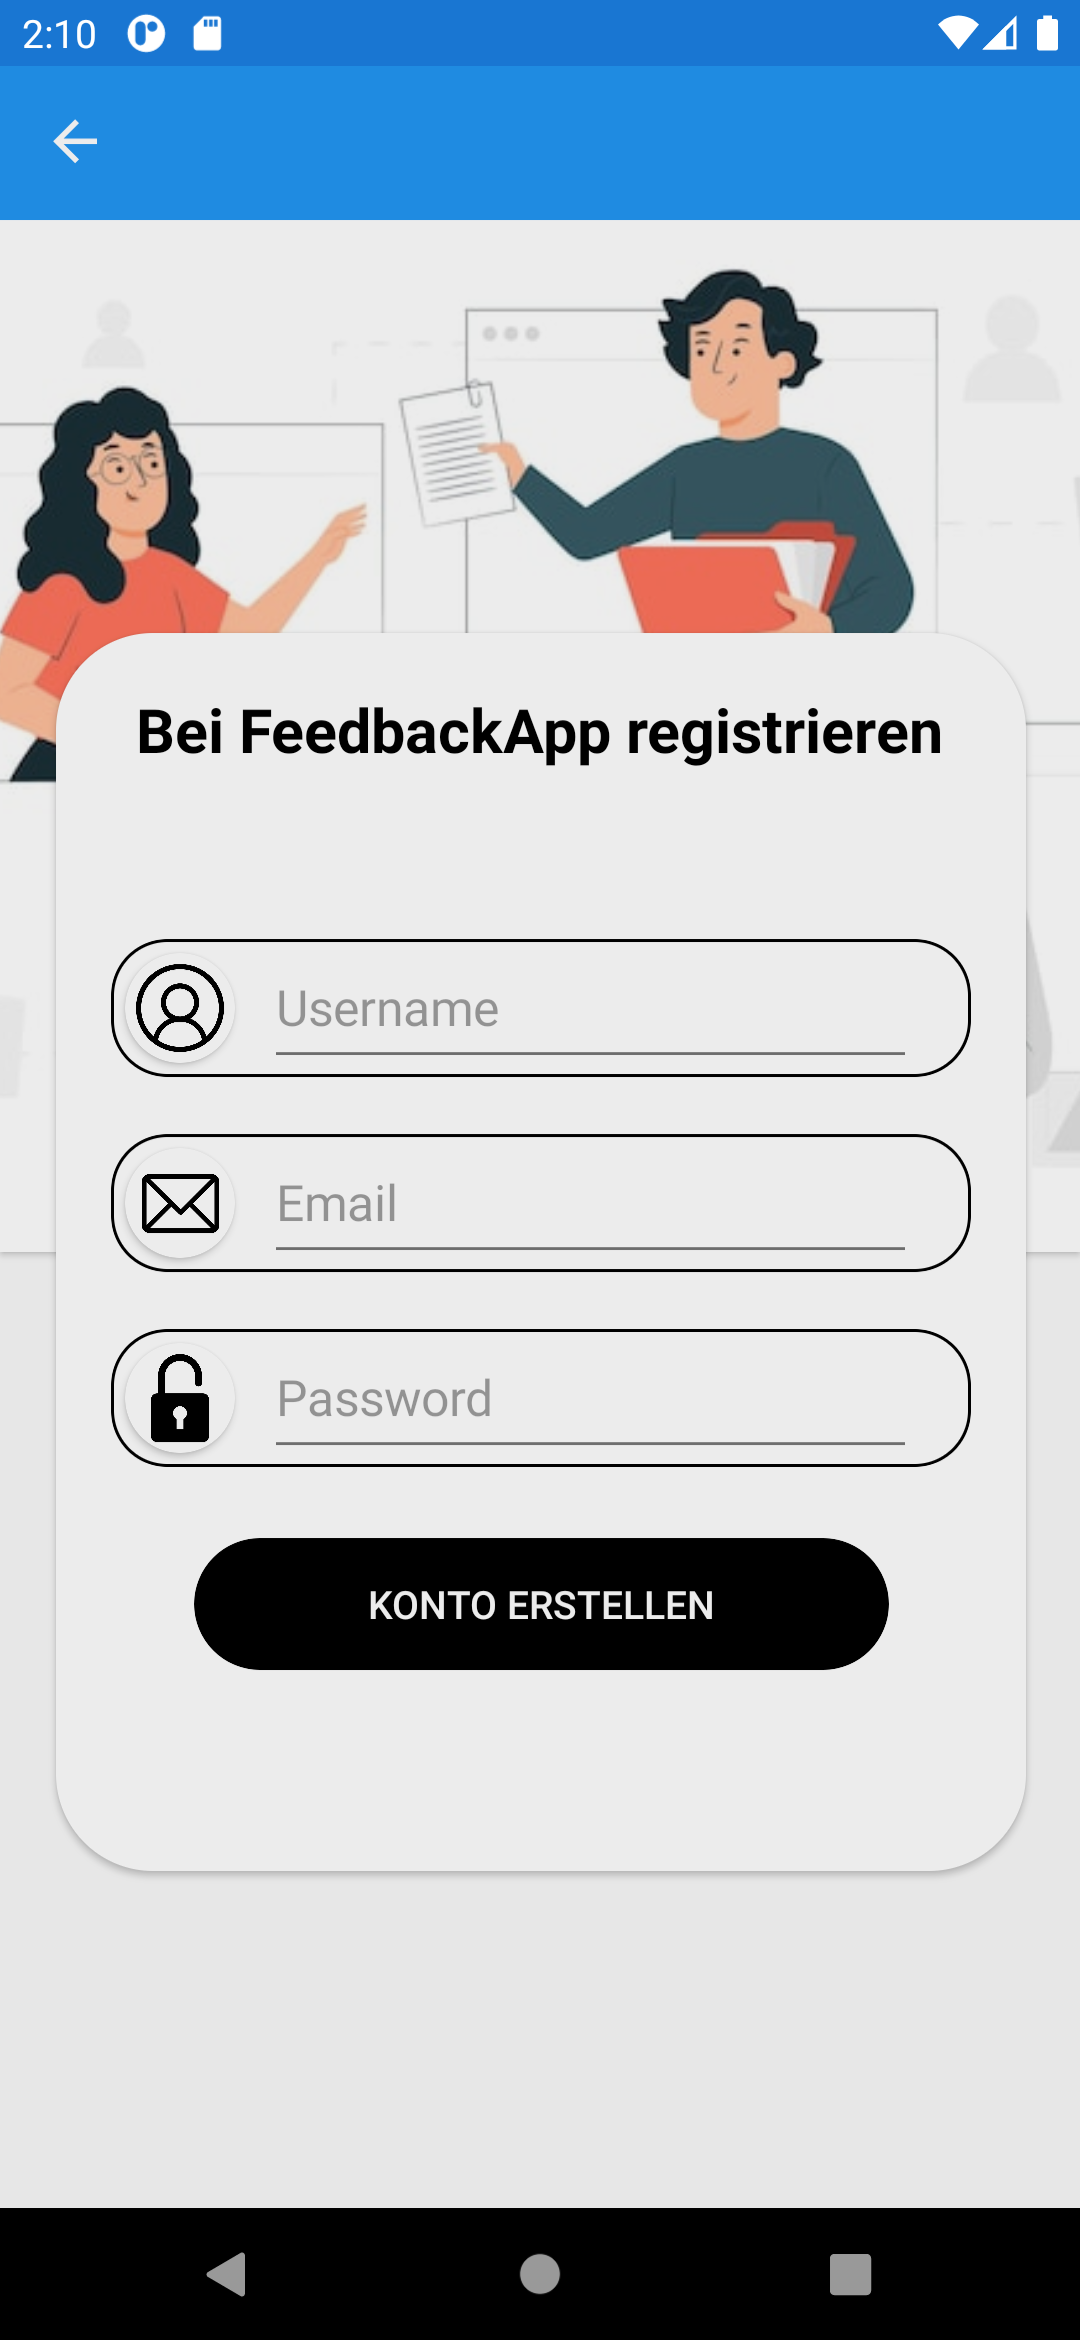
\includegraphics[width=5cm]{pics/Xamarin Student/2 Registration Page.png}
        \caption[Registrierung Ansicht]{Registrierung Page Ansicht}
    \end{center}
\end{figure}
Die Registrierungsseite ist einfach und übersichtlich gestaltet. Um einen Benutzer zu registrieren, müssen Sie einen Benutzernamen, eine E-Mail-Adresse und ein Passwort eingeben. Nur Schüler können sich mit dieser Methode registrieren, während die Lehrerregistrierung so geschützt ist, dass Schüler sich nicht als Lehrer registrieren können und Lehrer ihr Profil vom Admin-Team erhalten.
\newpage
\begin{figure}[h]
    \begin{center}
        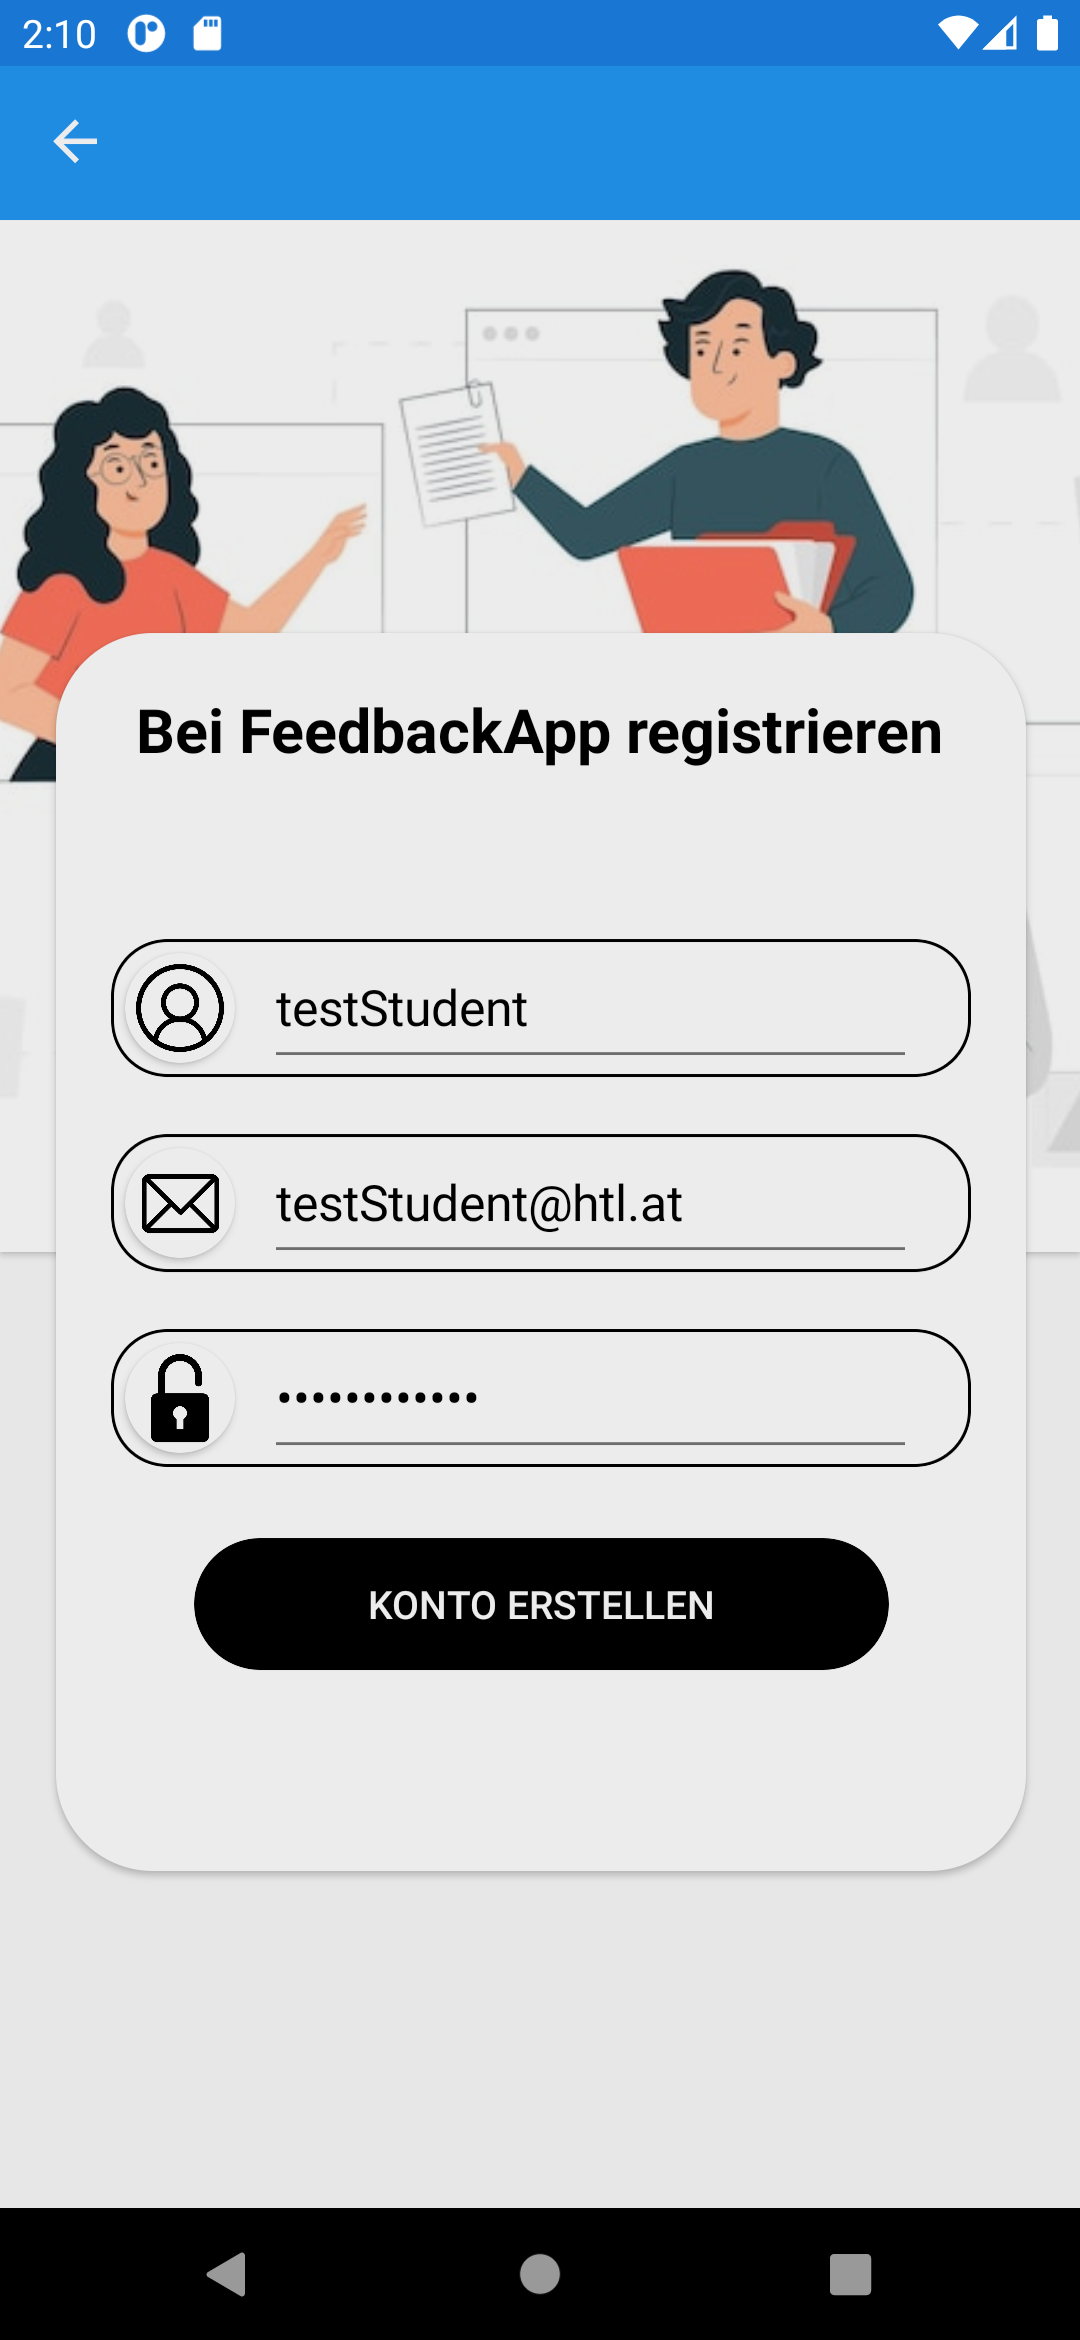
\includegraphics[width=4cm]{pics/Xamarin Student/3 Registration Page Full.png}\hfill
        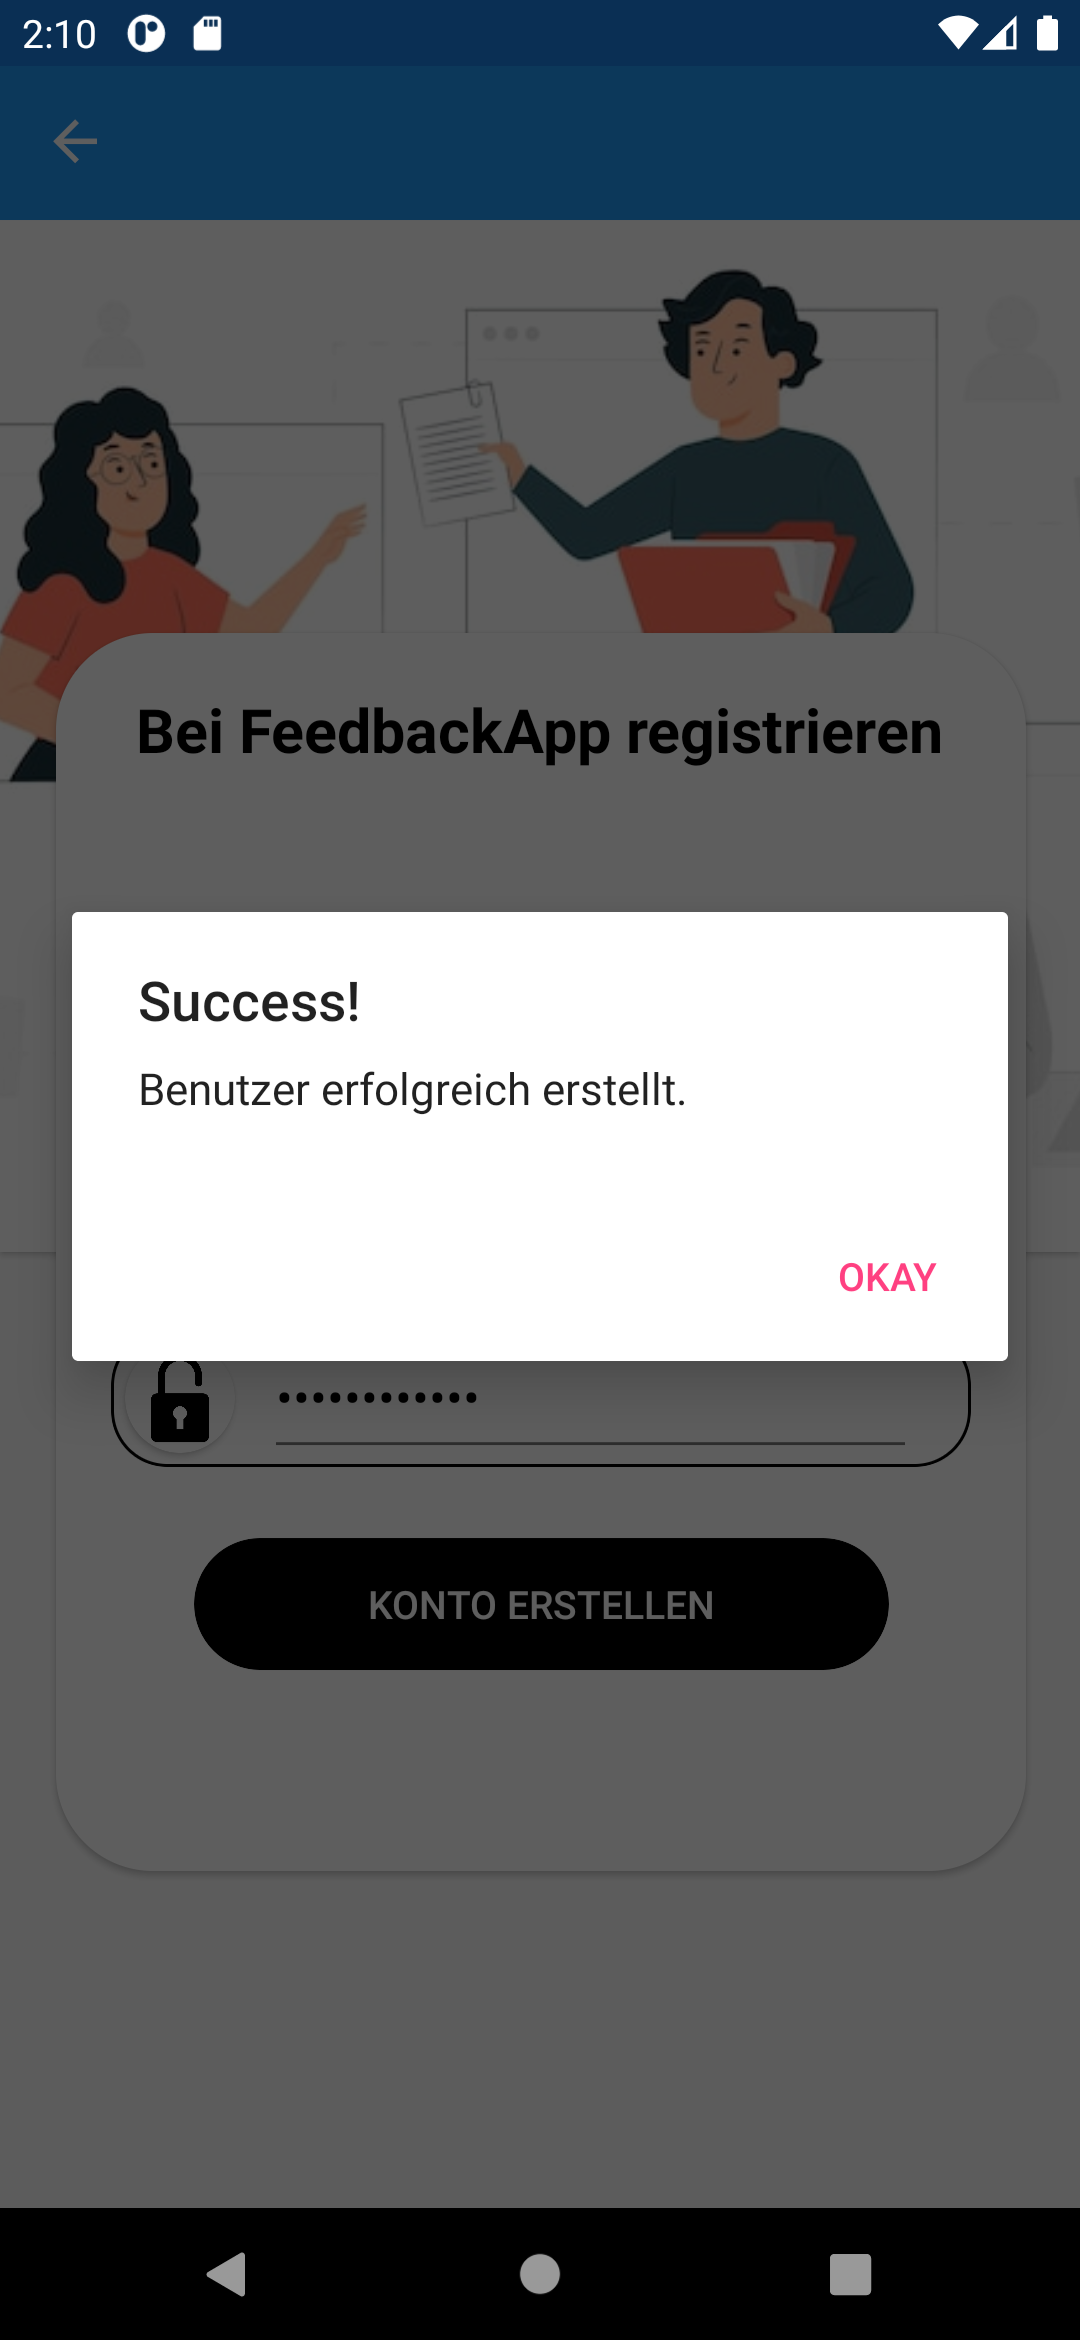
\includegraphics[width=4cm]{pics/Xamarin Student/4 Registration Page Success.png}
        \caption[Registrierung Ansicht]{Benutzerkonto erstellen}
    \end{center}
\end{figure}
Falls die Daten falsch sind, d.h. die nicht den Regeln des Codes unterliegen, erhalten wir per E-Mail eine Warnung und einen Fehler, um die Registrierungsaktion zu wiederholen.
\newpage

\section{Benutzerkontoverwaltung}
Im Profil kann der Benutzer seine gespeicherten Daten wie Passwort, Vorname oder
Schule aktualisieren.
Die Seite ist einfach und geräumig gestaltet, um die Daten, die der Benutzer benötigt, klar zu sehen.
\vspace{2cm}
\begin{figure}[h]
    \begin{center}
        \includegraphics*[width=5cm]{pics/Xamarin Student/13 My Acc.png}
        \caption[MyAccount Ansicht]{Benutzerkontoverwaltung Student Ansicht}
    \end{center}
\end{figure}
\newpage
Sobald wir die Benutzerkontoseite betreten, sehen wir, dass der Name, der Nachname und der Name der Schule, die wir besuchen, fehlt. Mit den Buttons auf der rechten Seite können wir jeden einzeln eingeben, ändern oder löschen. Auch die E-Mail ist bereits gespeichert, die wir bei der Registrierung eingegeben haben, die aber später geändert werden kann.
\newline
\begin{figure}[h]
    \begin{center}
    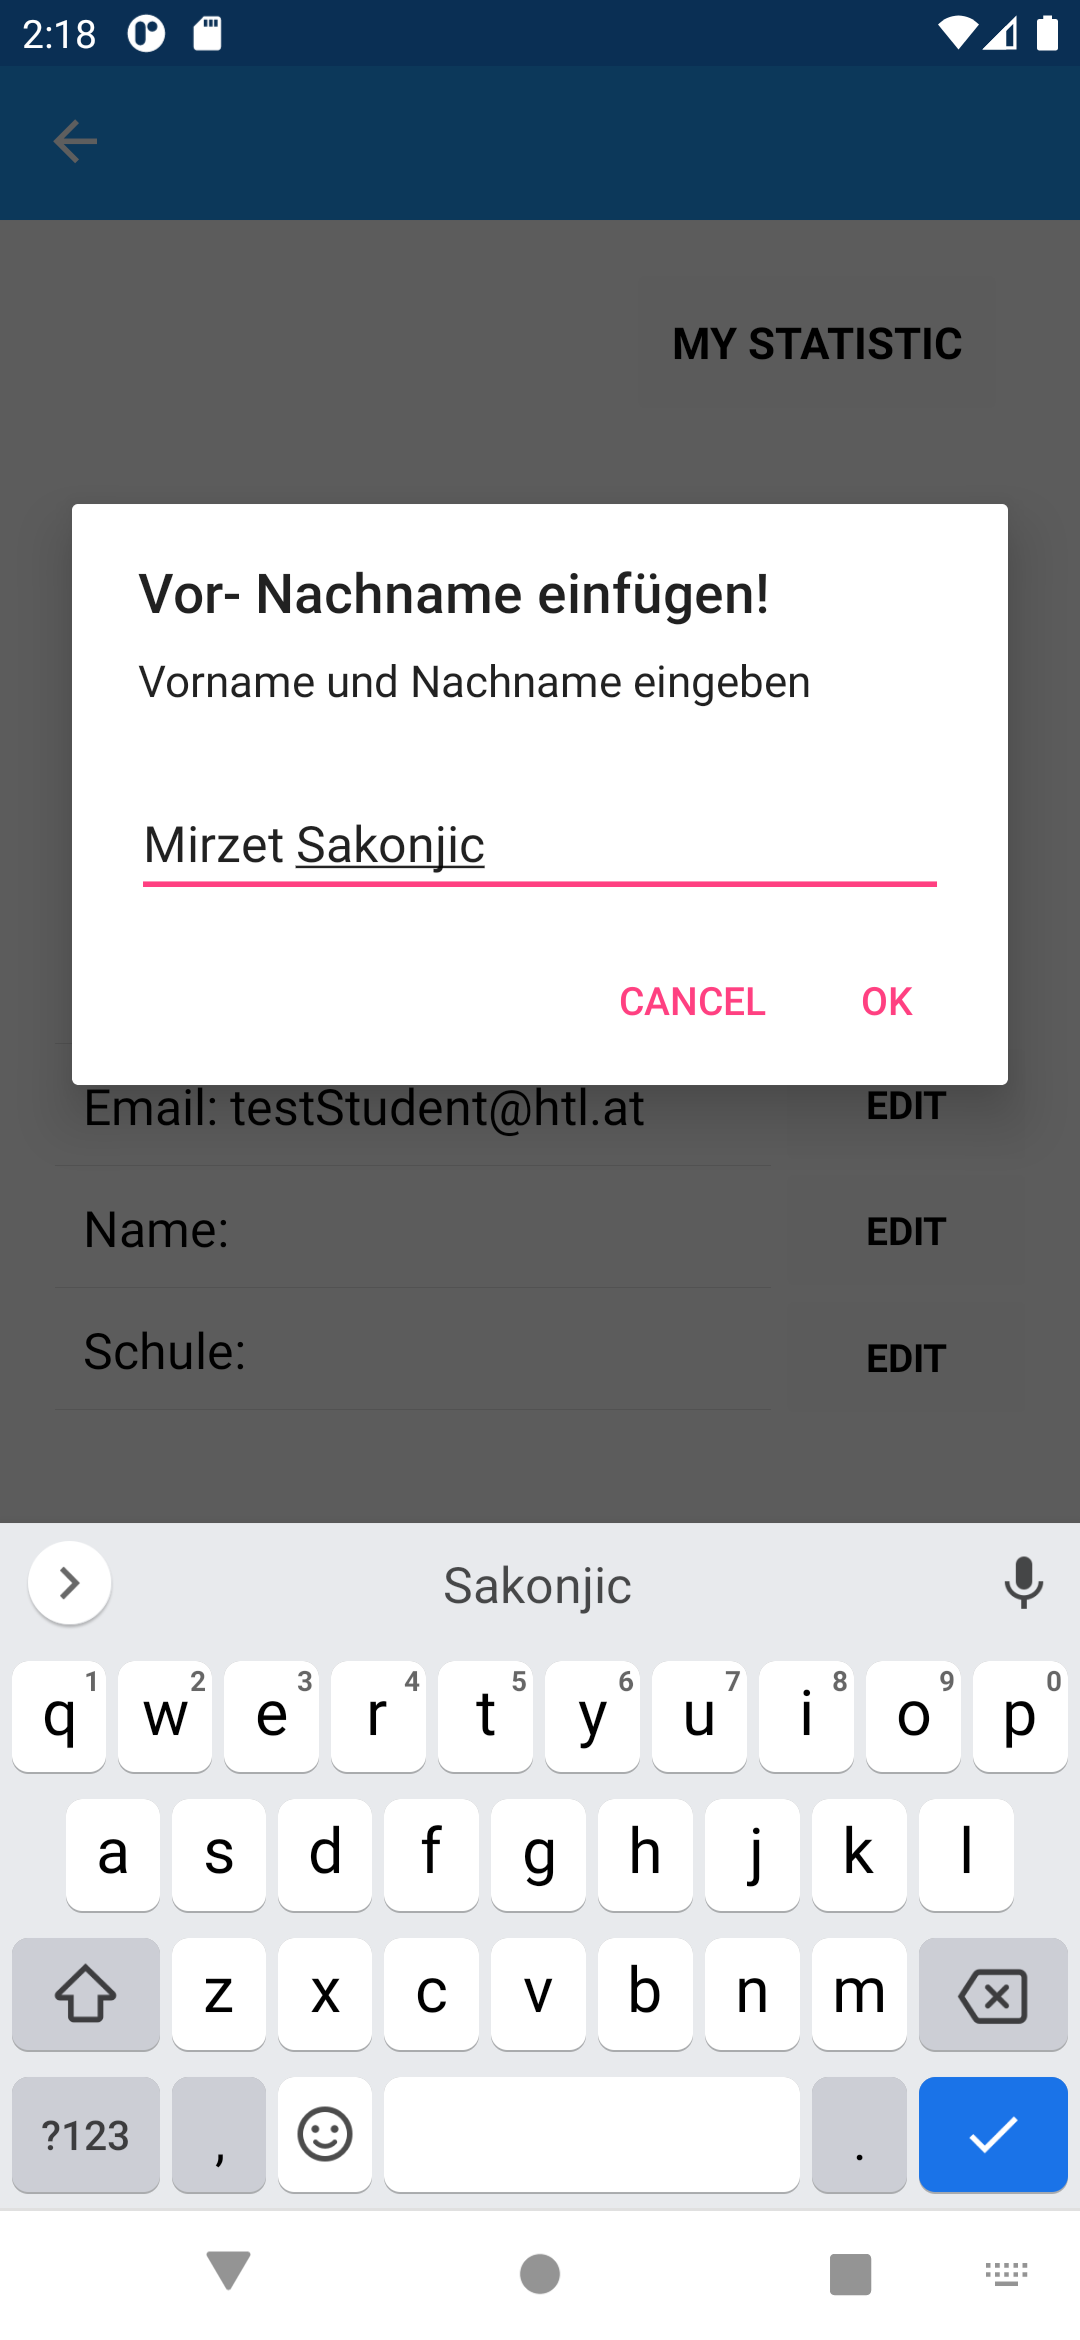
\includegraphics[width=5cm]{pics/Xamarin Student/14 Name.png}\hfill
    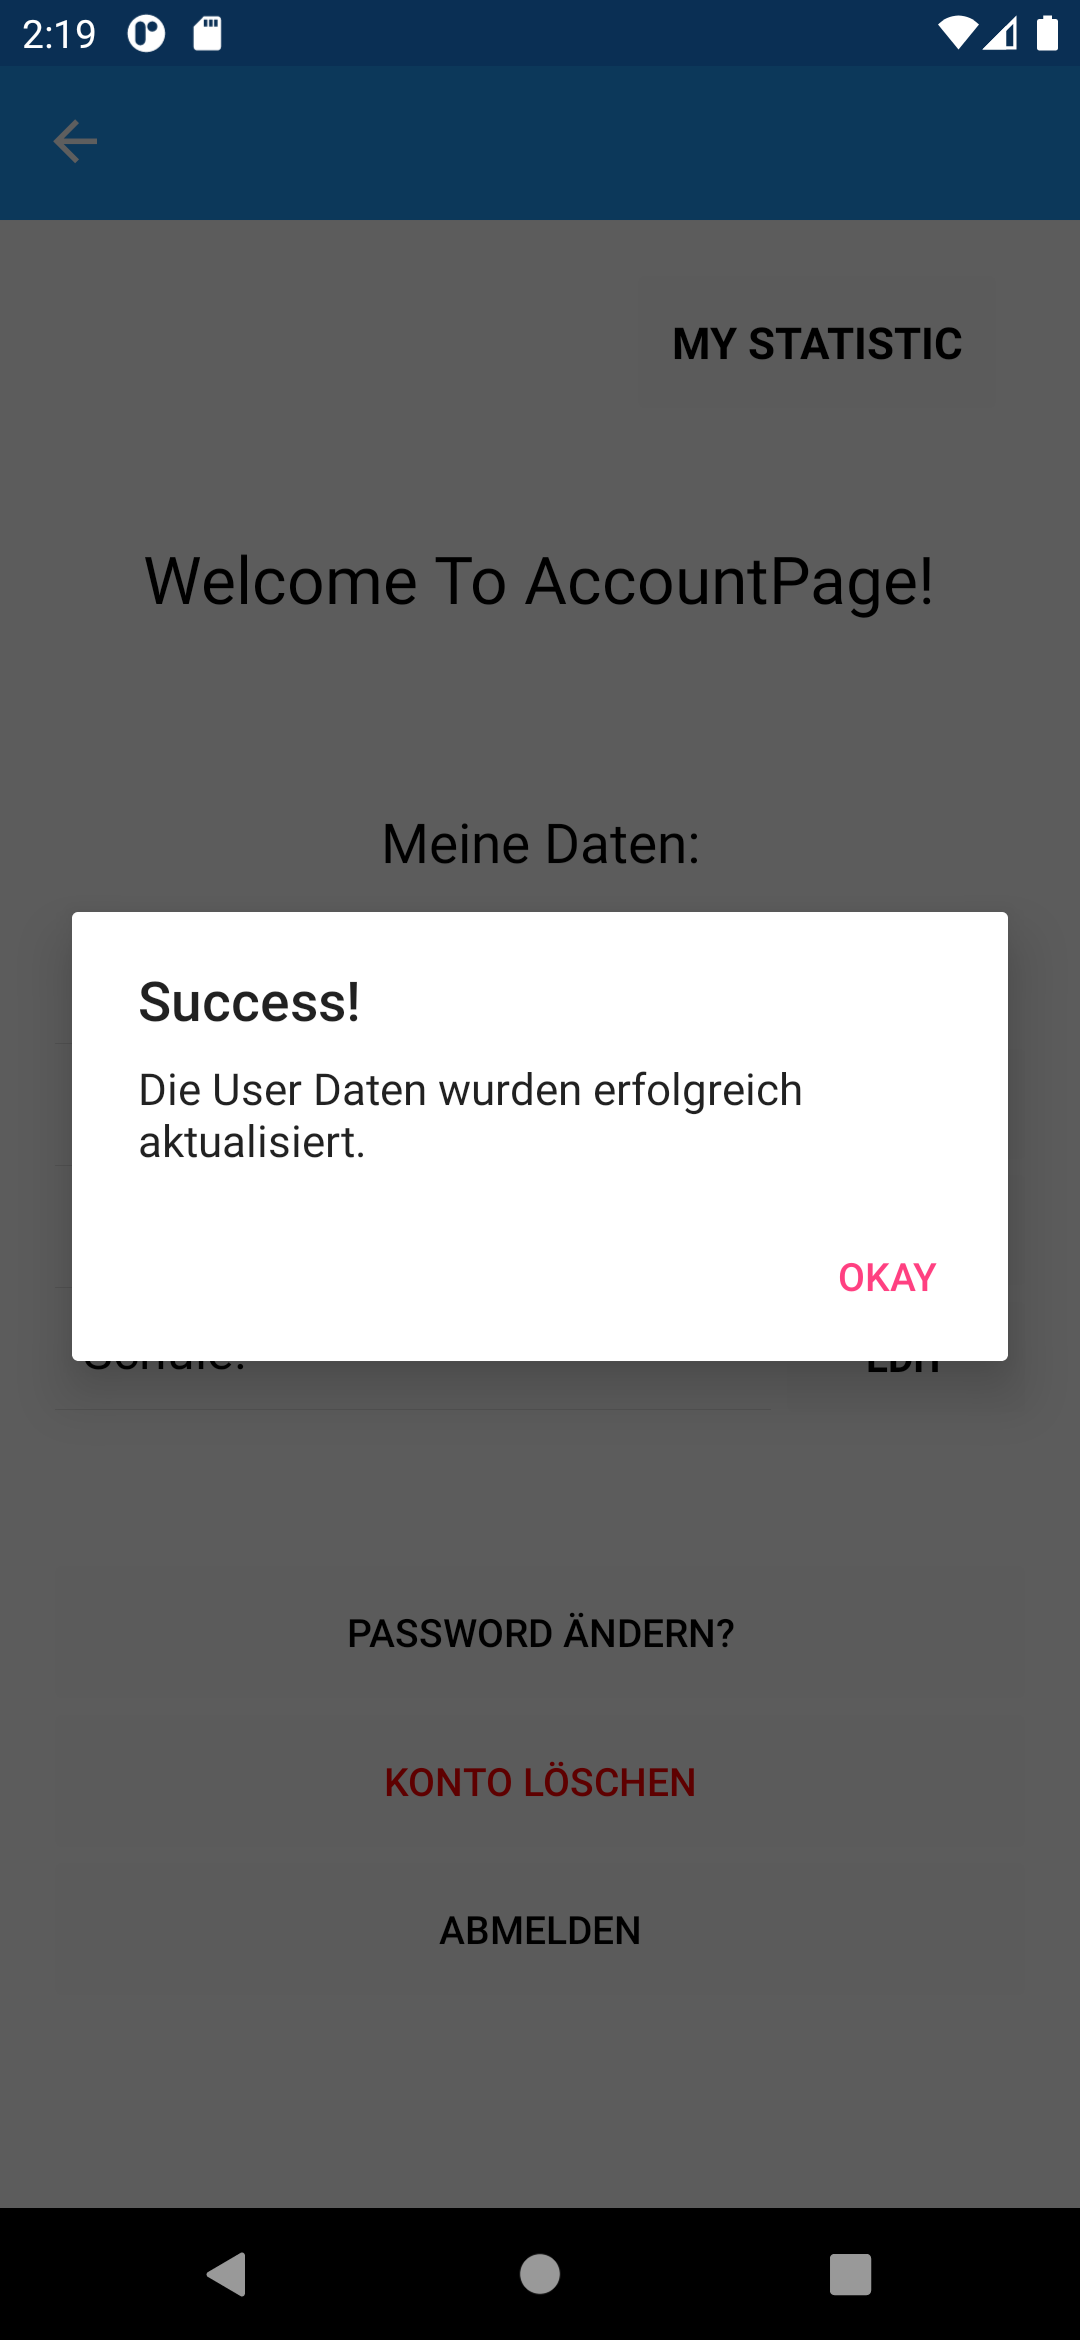
\includegraphics[width=5cm]{pics/Xamarin Student/15 Name success.png}\hfill
    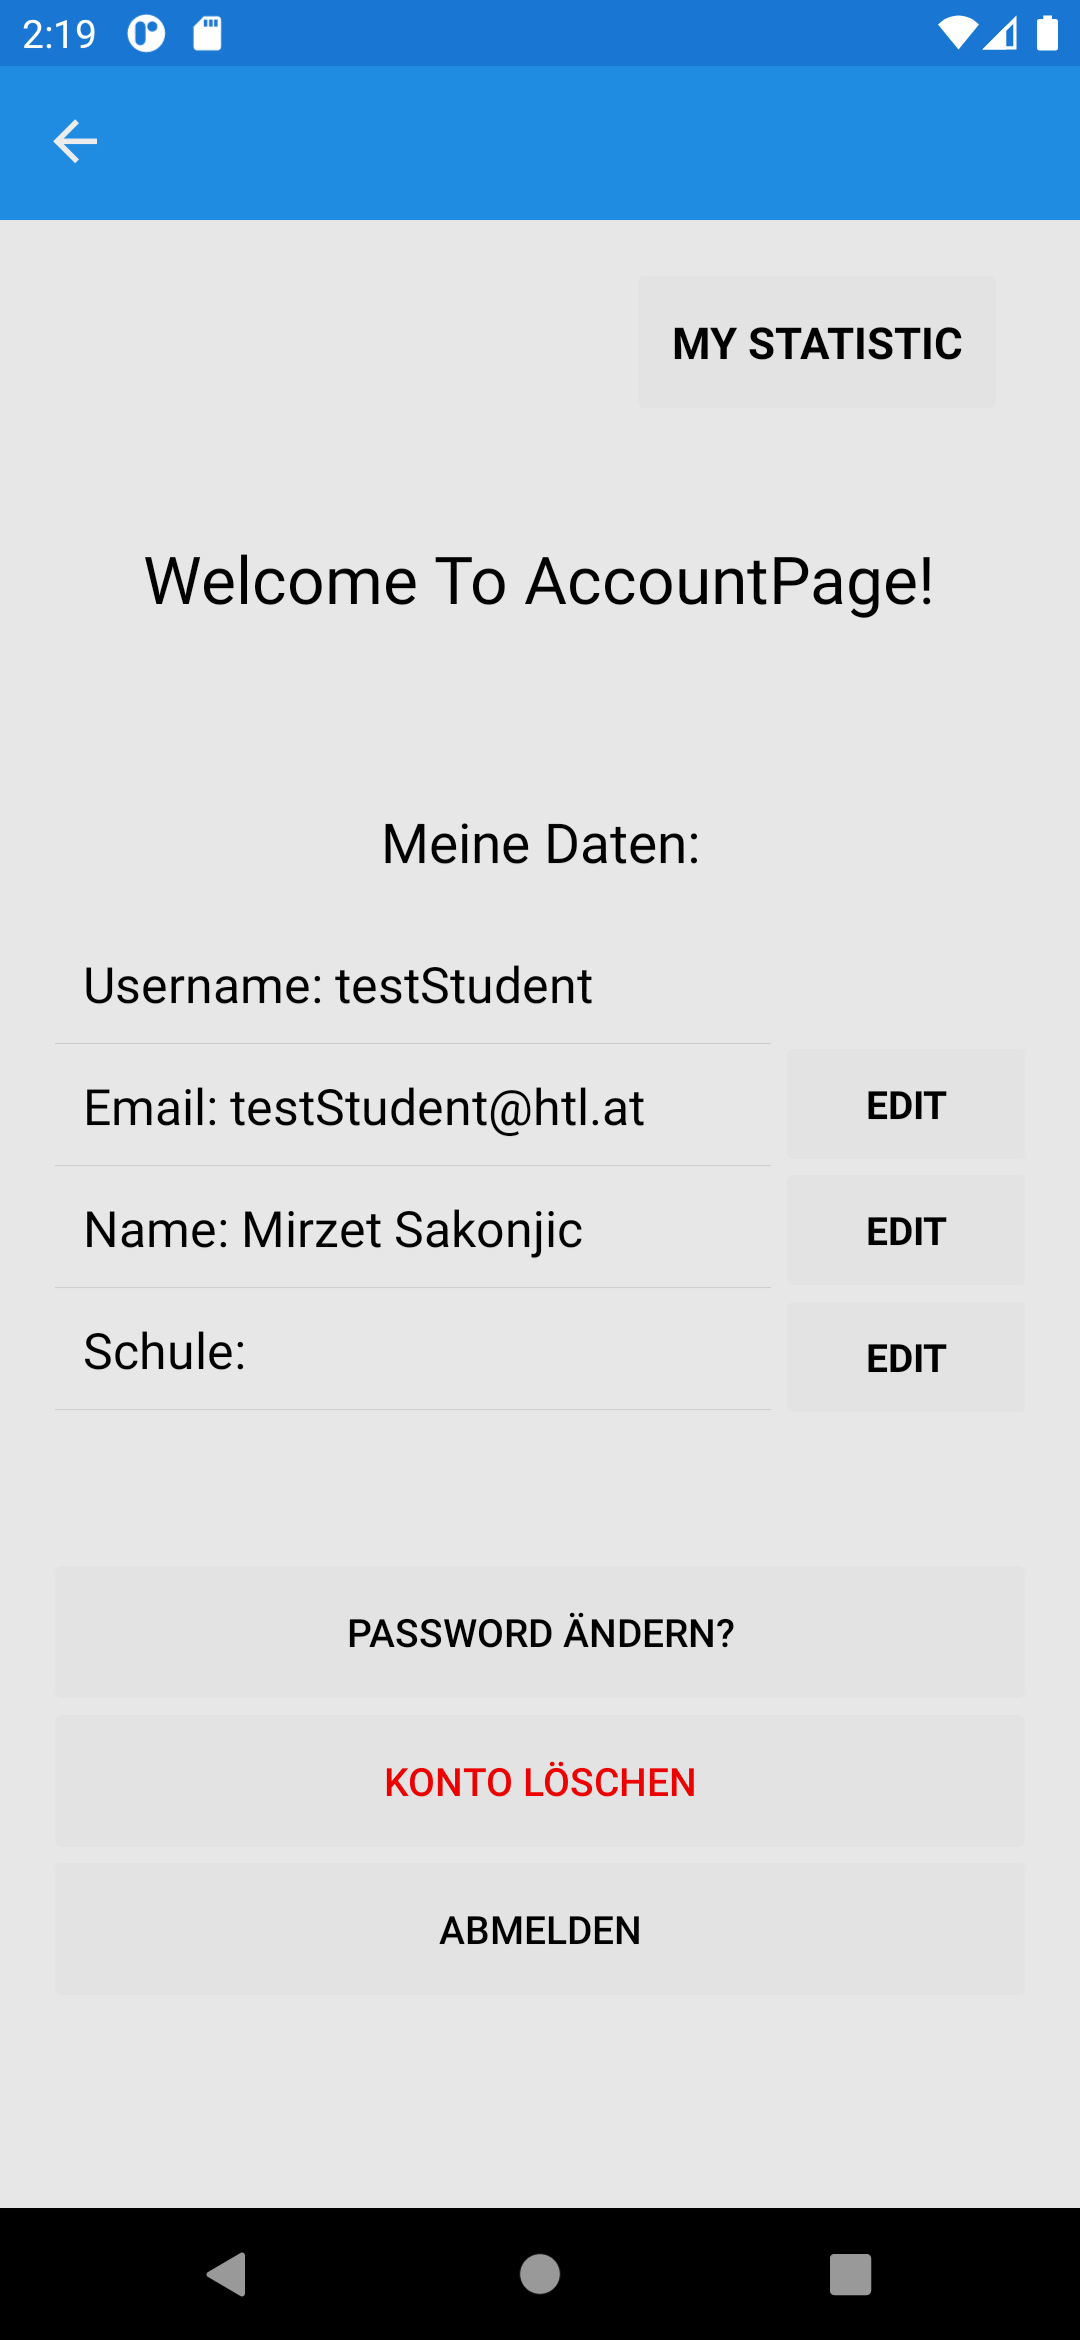
\includegraphics[width=5cm]{pics/Xamarin Student/16 Name.png}
    \caption[MyAccount Namensänderung]{Namensänderung}
    \end{center}
\end{figure}
\newpage
Als nächstes geben Sie den Namen der Schule ein, die wir besuchen, oder des Hauptfachs, das wir studieren.
\begin{figure}[h]
    \begin{center}
    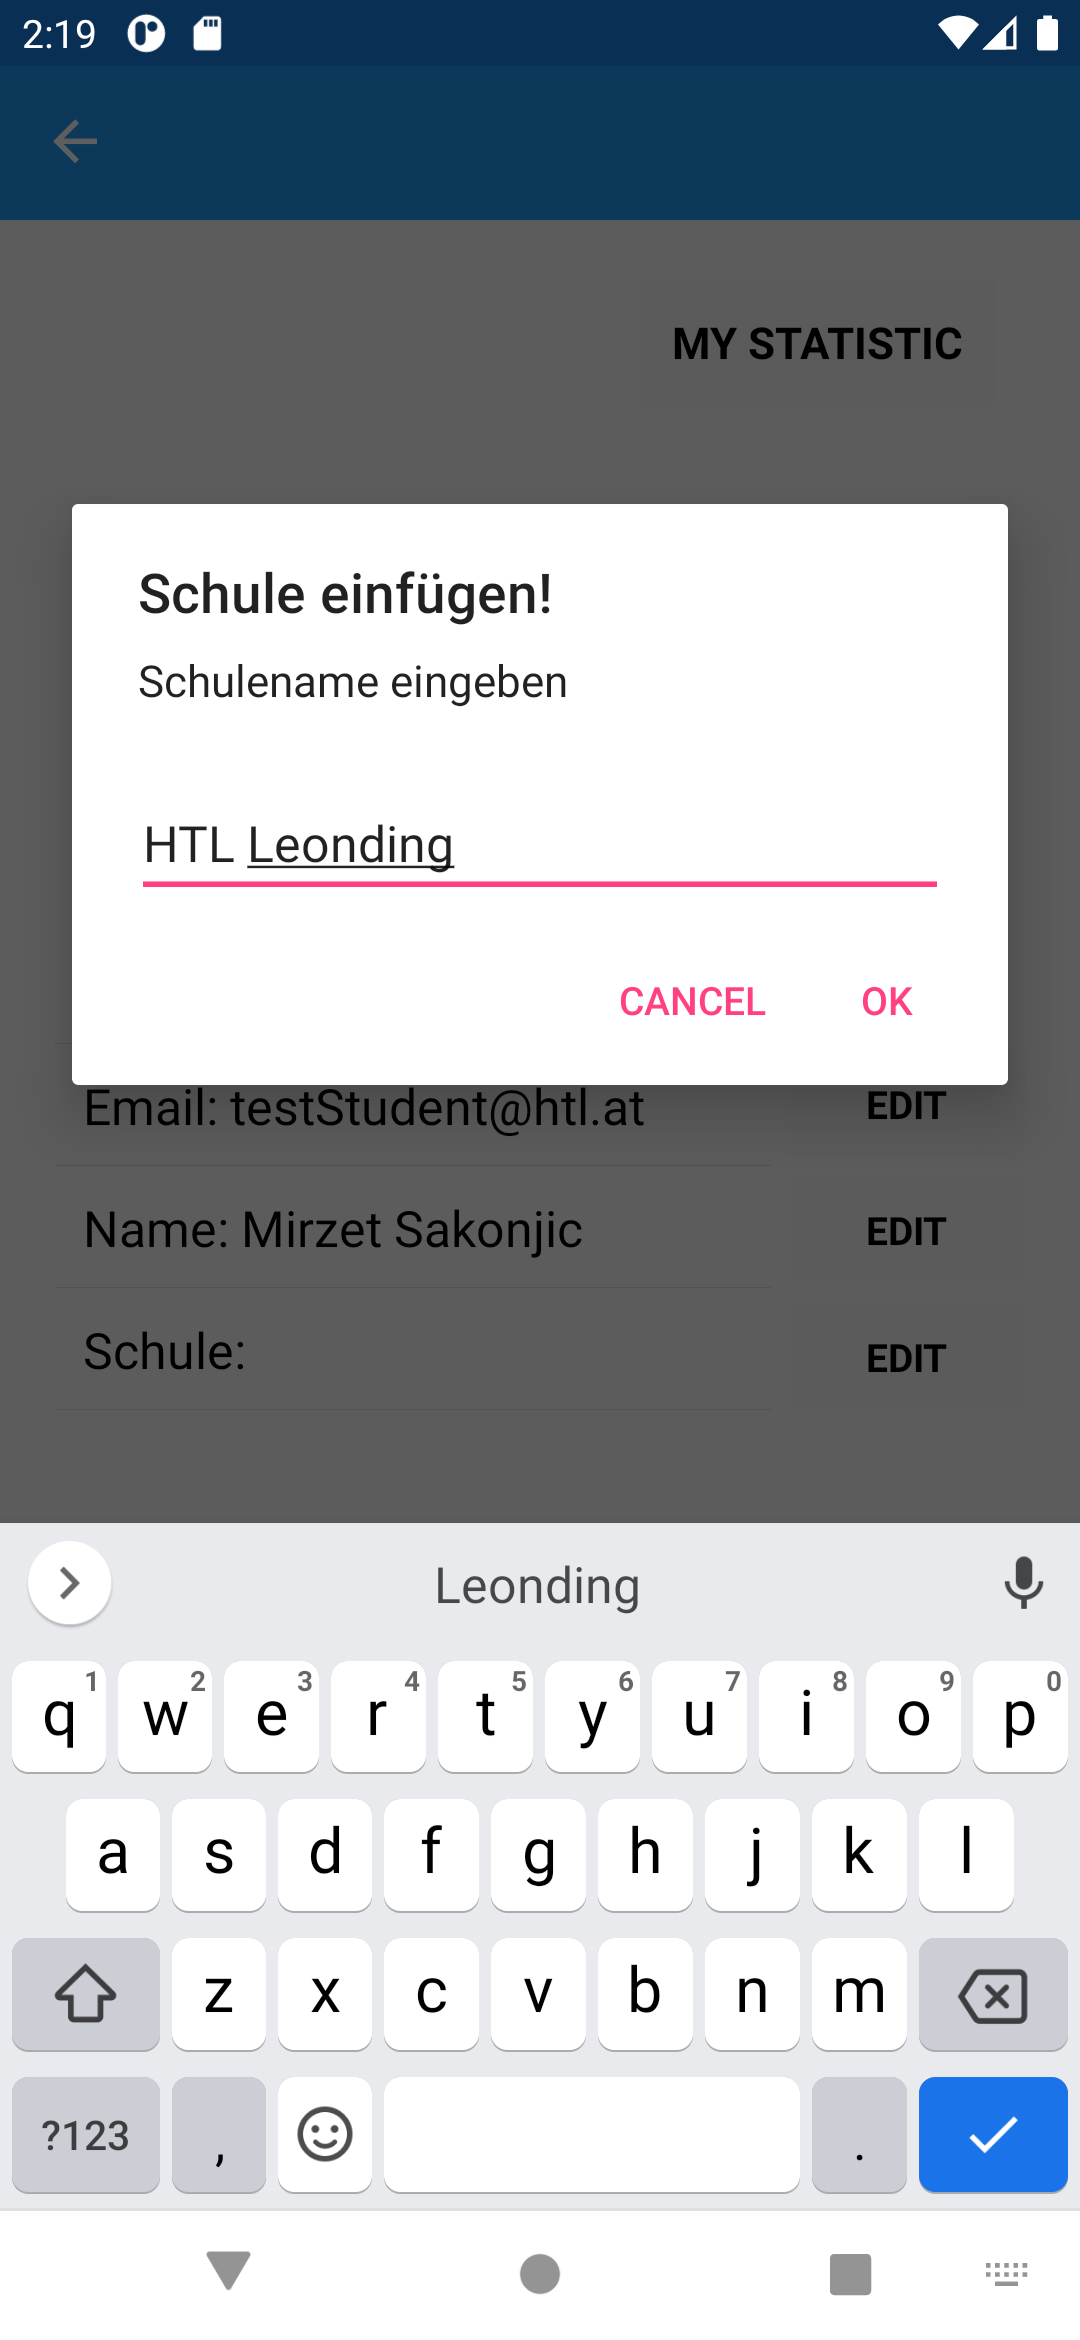
\includegraphics[width=5cm]{pics/Xamarin Student/17 School.png}\hfill
    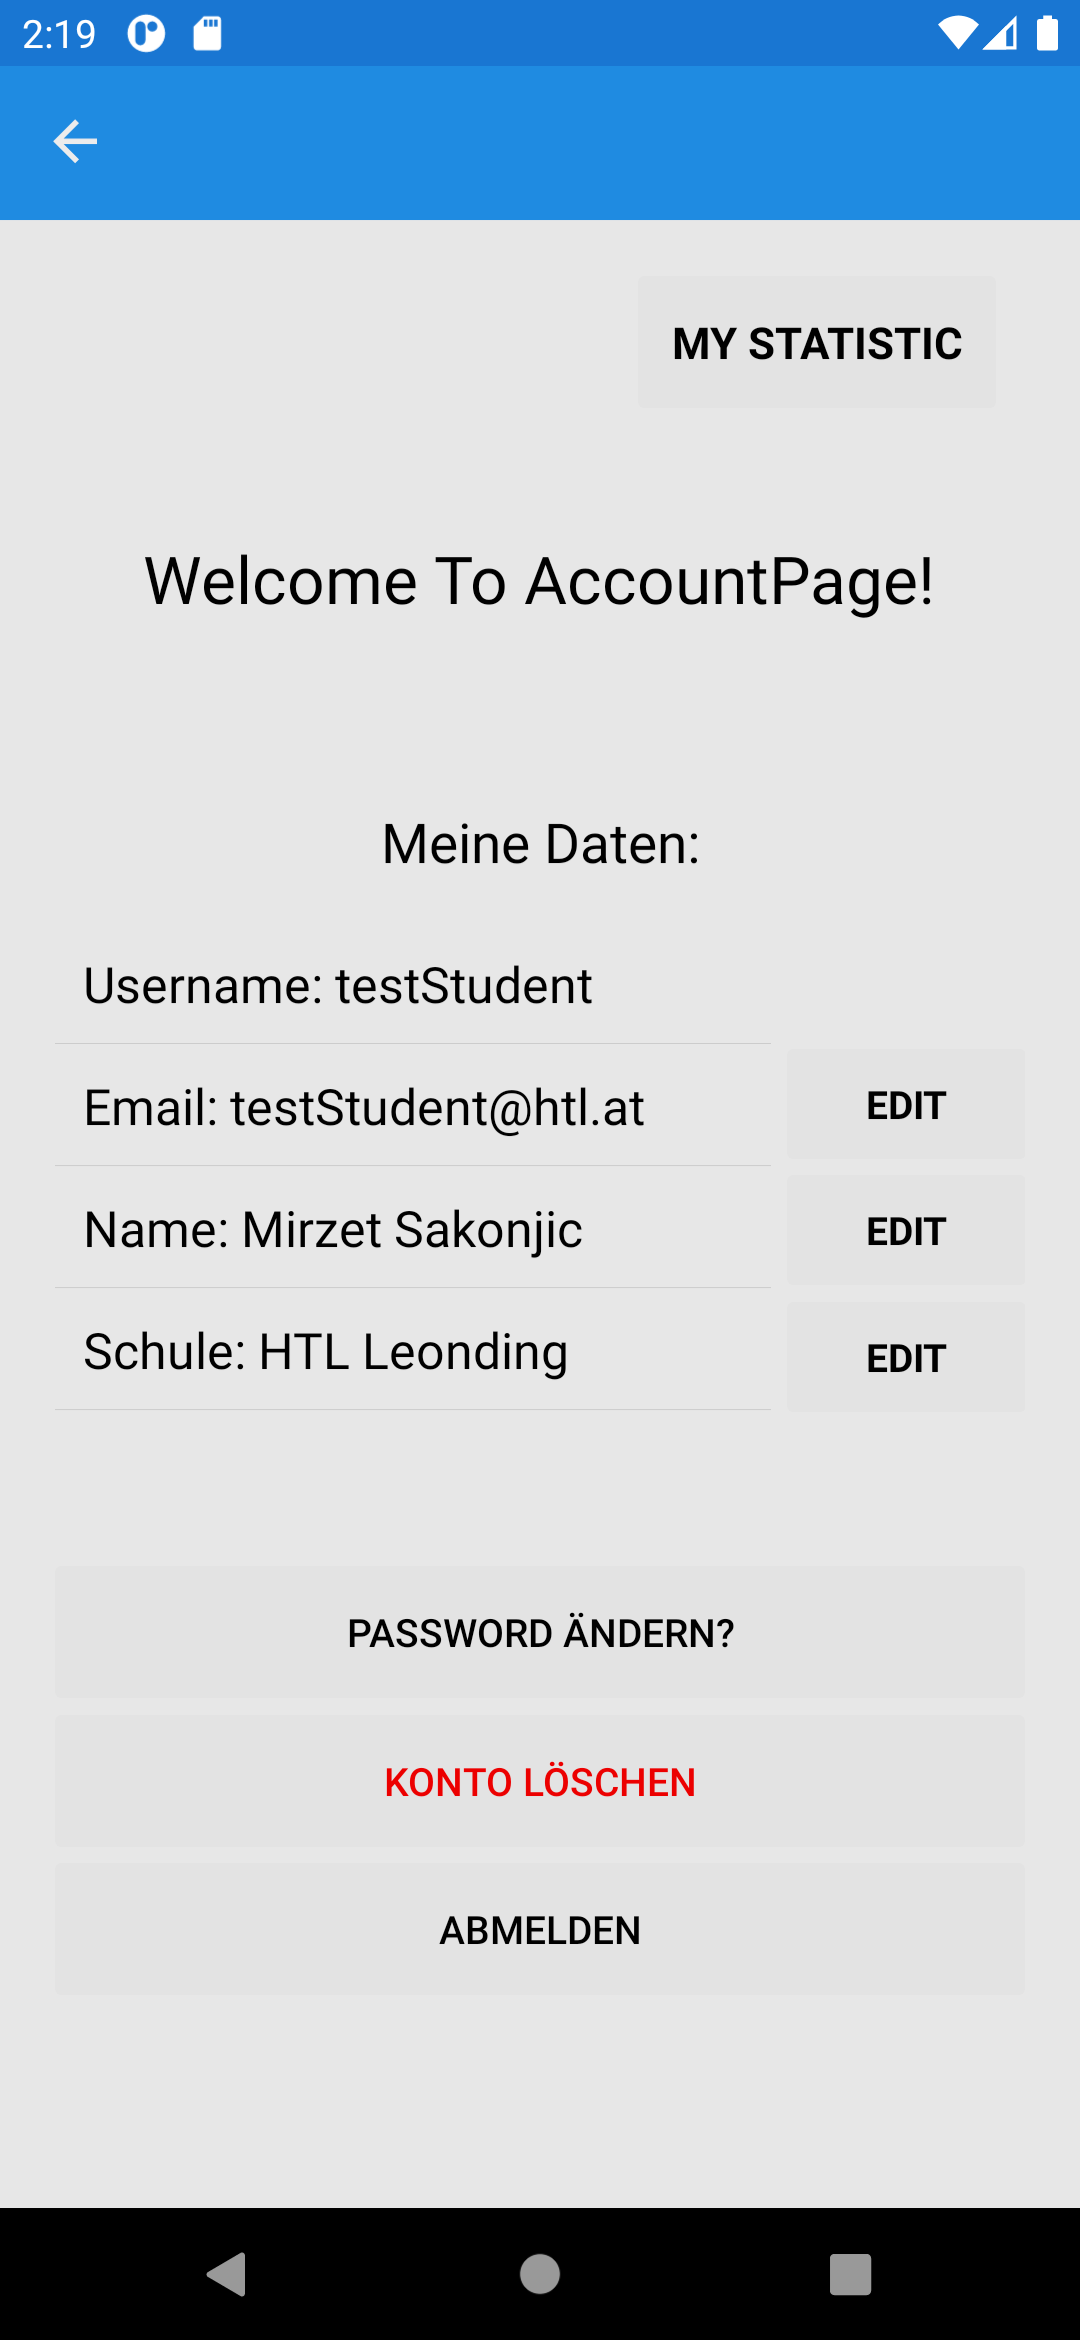
\includegraphics[width=5cm]{pics/Xamarin Student/18 School success.png}
    \caption[MyAccount Umbenennung der Schule]{Umbenennung der Schule}
    \end{center}
\end{figure}
\newline
Falls wir die E-Mail-Adresse ändern und eine neue eingeben möchten, ist dies ebenfalls möglich. Falls die neue E-Mail-Adresse falsch ist oder die Kriterien für die E-Mail-Adresse nicht erfüllt, erhalten wir eine Fehlermeldung.
\begin{figure}[h]
    \begin{center}
    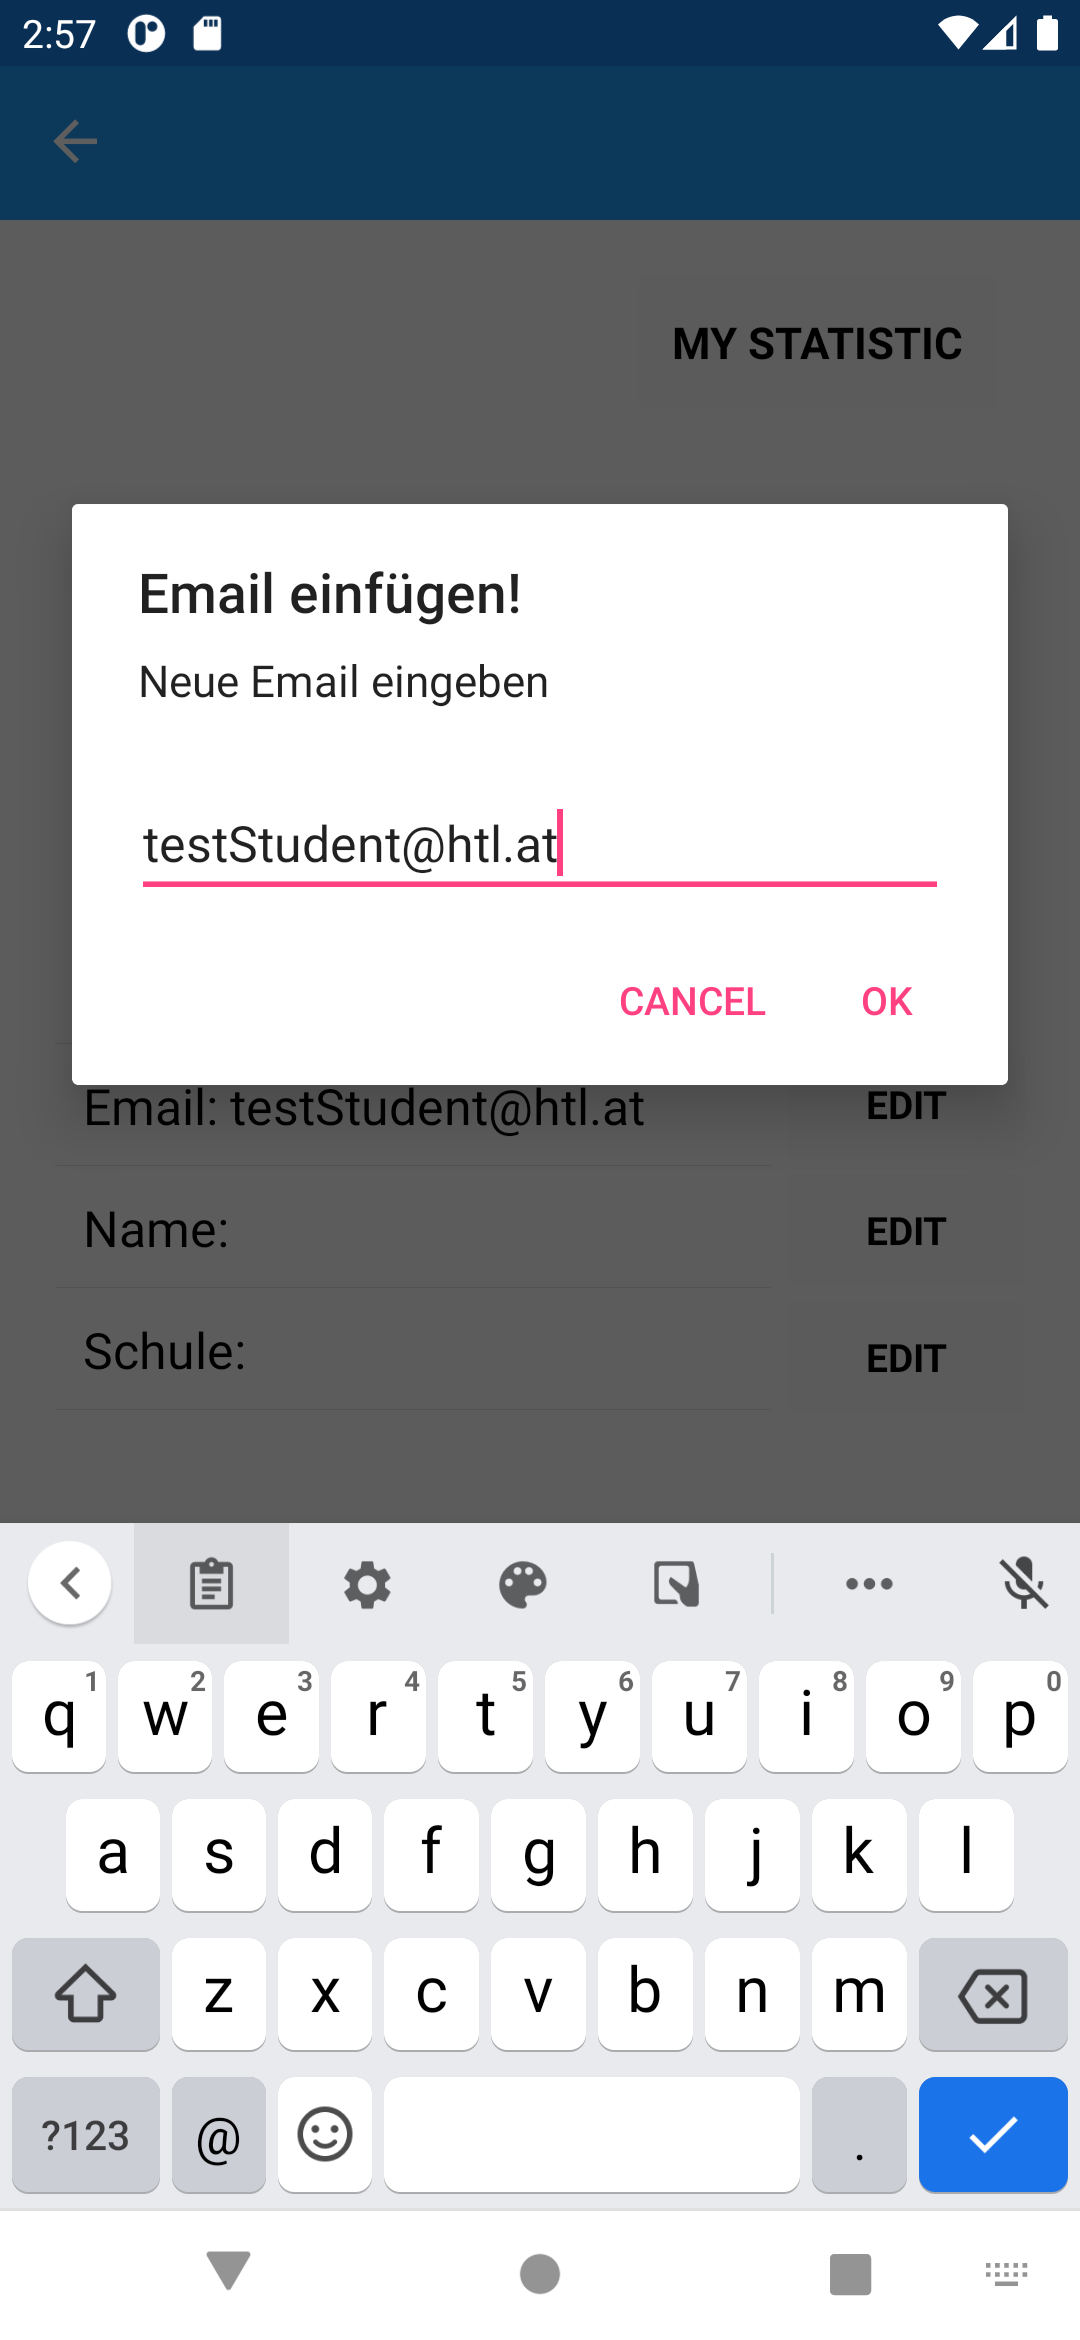
\includegraphics[width=5cm]{pics/Xamarin Student/26 New Email.png}\
    \caption[MyAccount Änderung der E-Mail-Adresse]{Änderung der E-Mail-Adresse}
    \end{center}
\end{figure}
\newpage
Wir werden das Passwort ändern, indem wir zuerst das alte Passwort und dann das neue eingeben. Wenn das alte Passwort korrekt ist und somit das neue Passwort den Passwortkriterien unterliegt, wird das neue Passwort gespeichert.
\begin{figure}[h]
    \begin{center}
    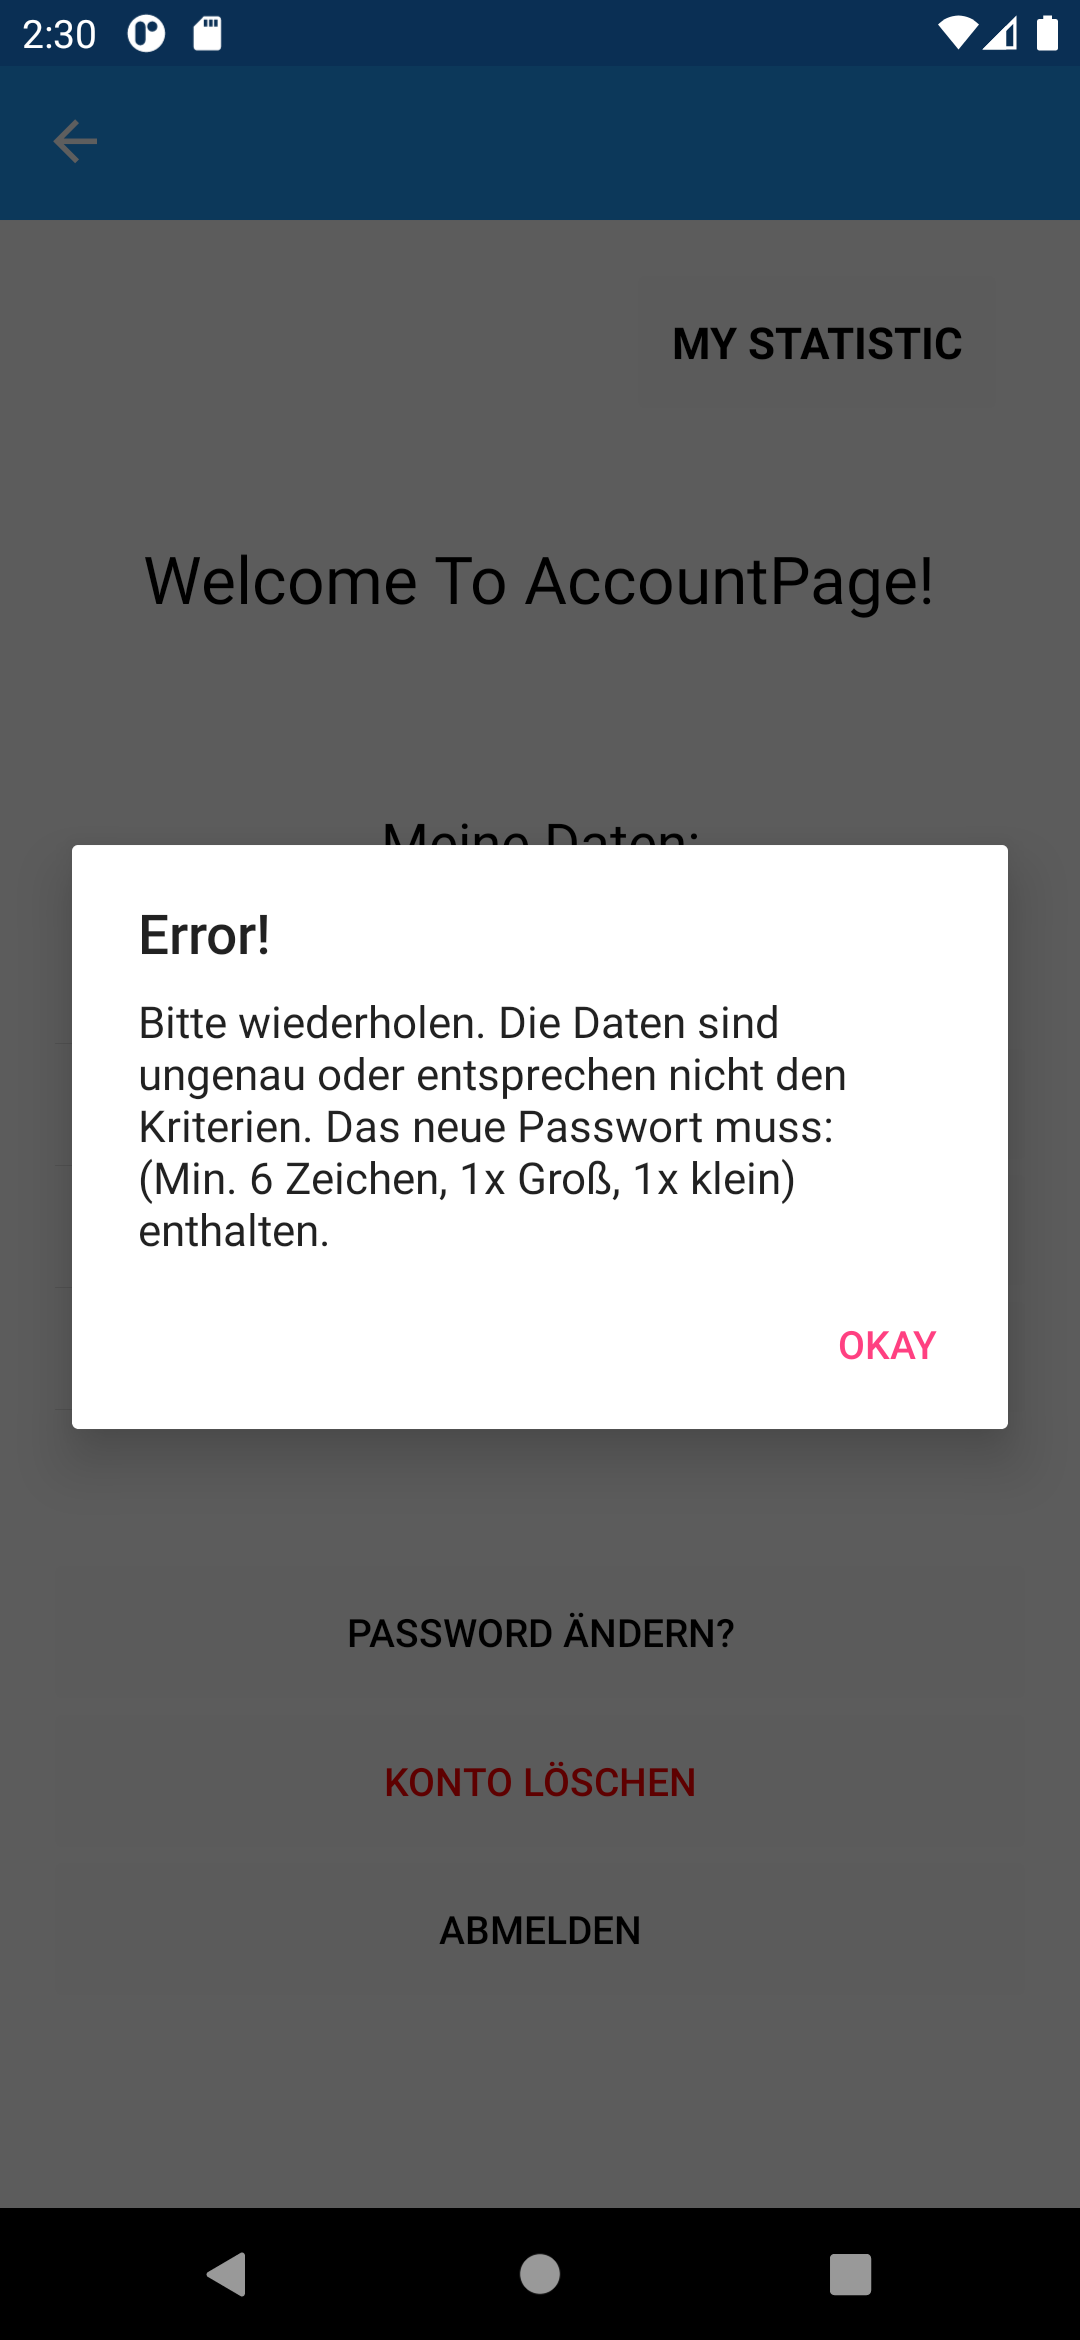
\includegraphics[width=5cm]{pics/Xamarin Student/19 Pass change.png}\hfill
    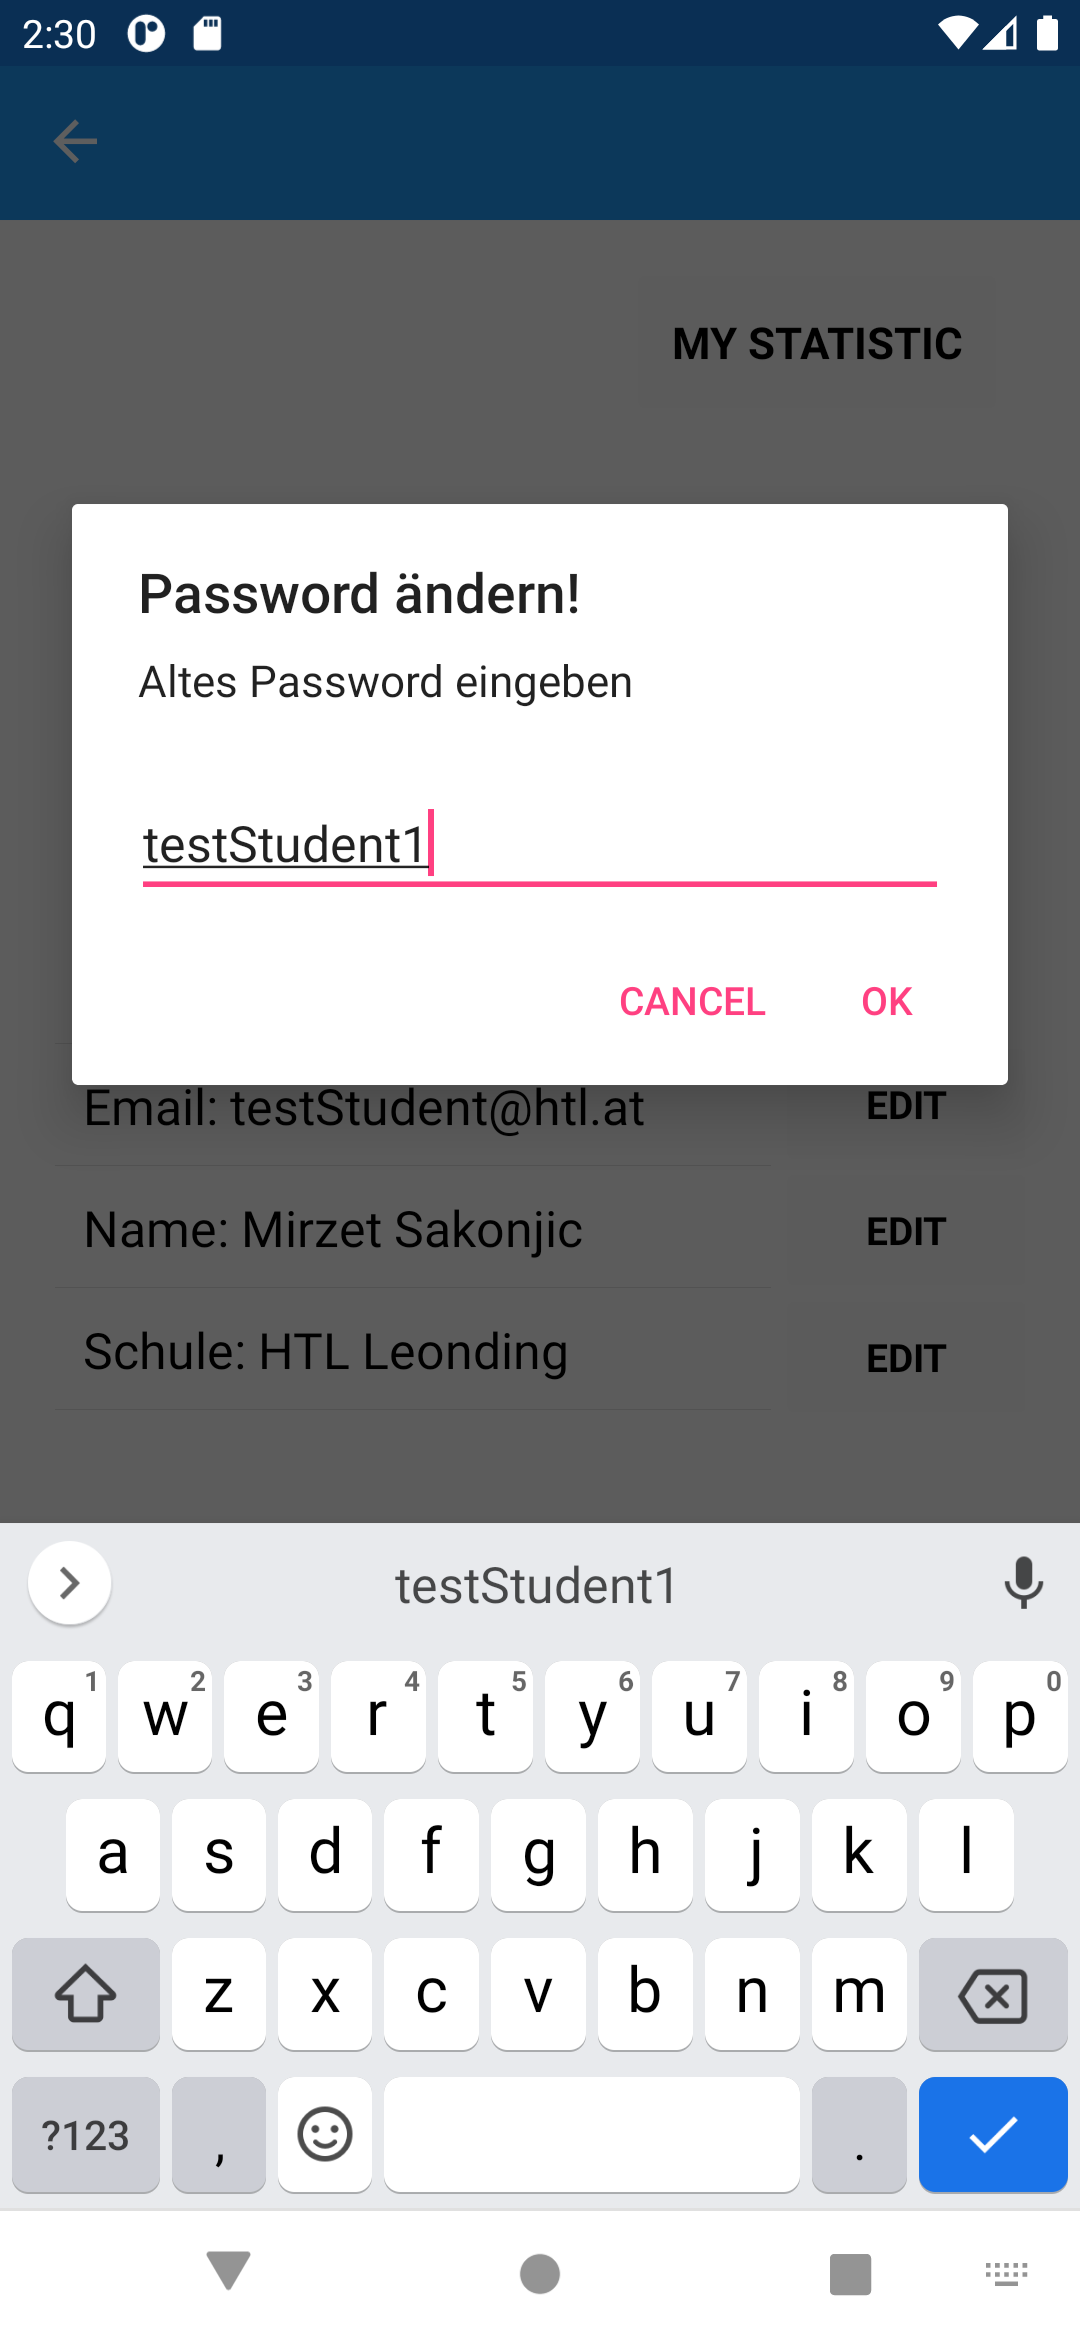
\includegraphics[width=5cm]{pics/Xamarin Student/20.png}
    \end{center}
\end{figure}
\begin{figure}[h]
    \begin{center}
    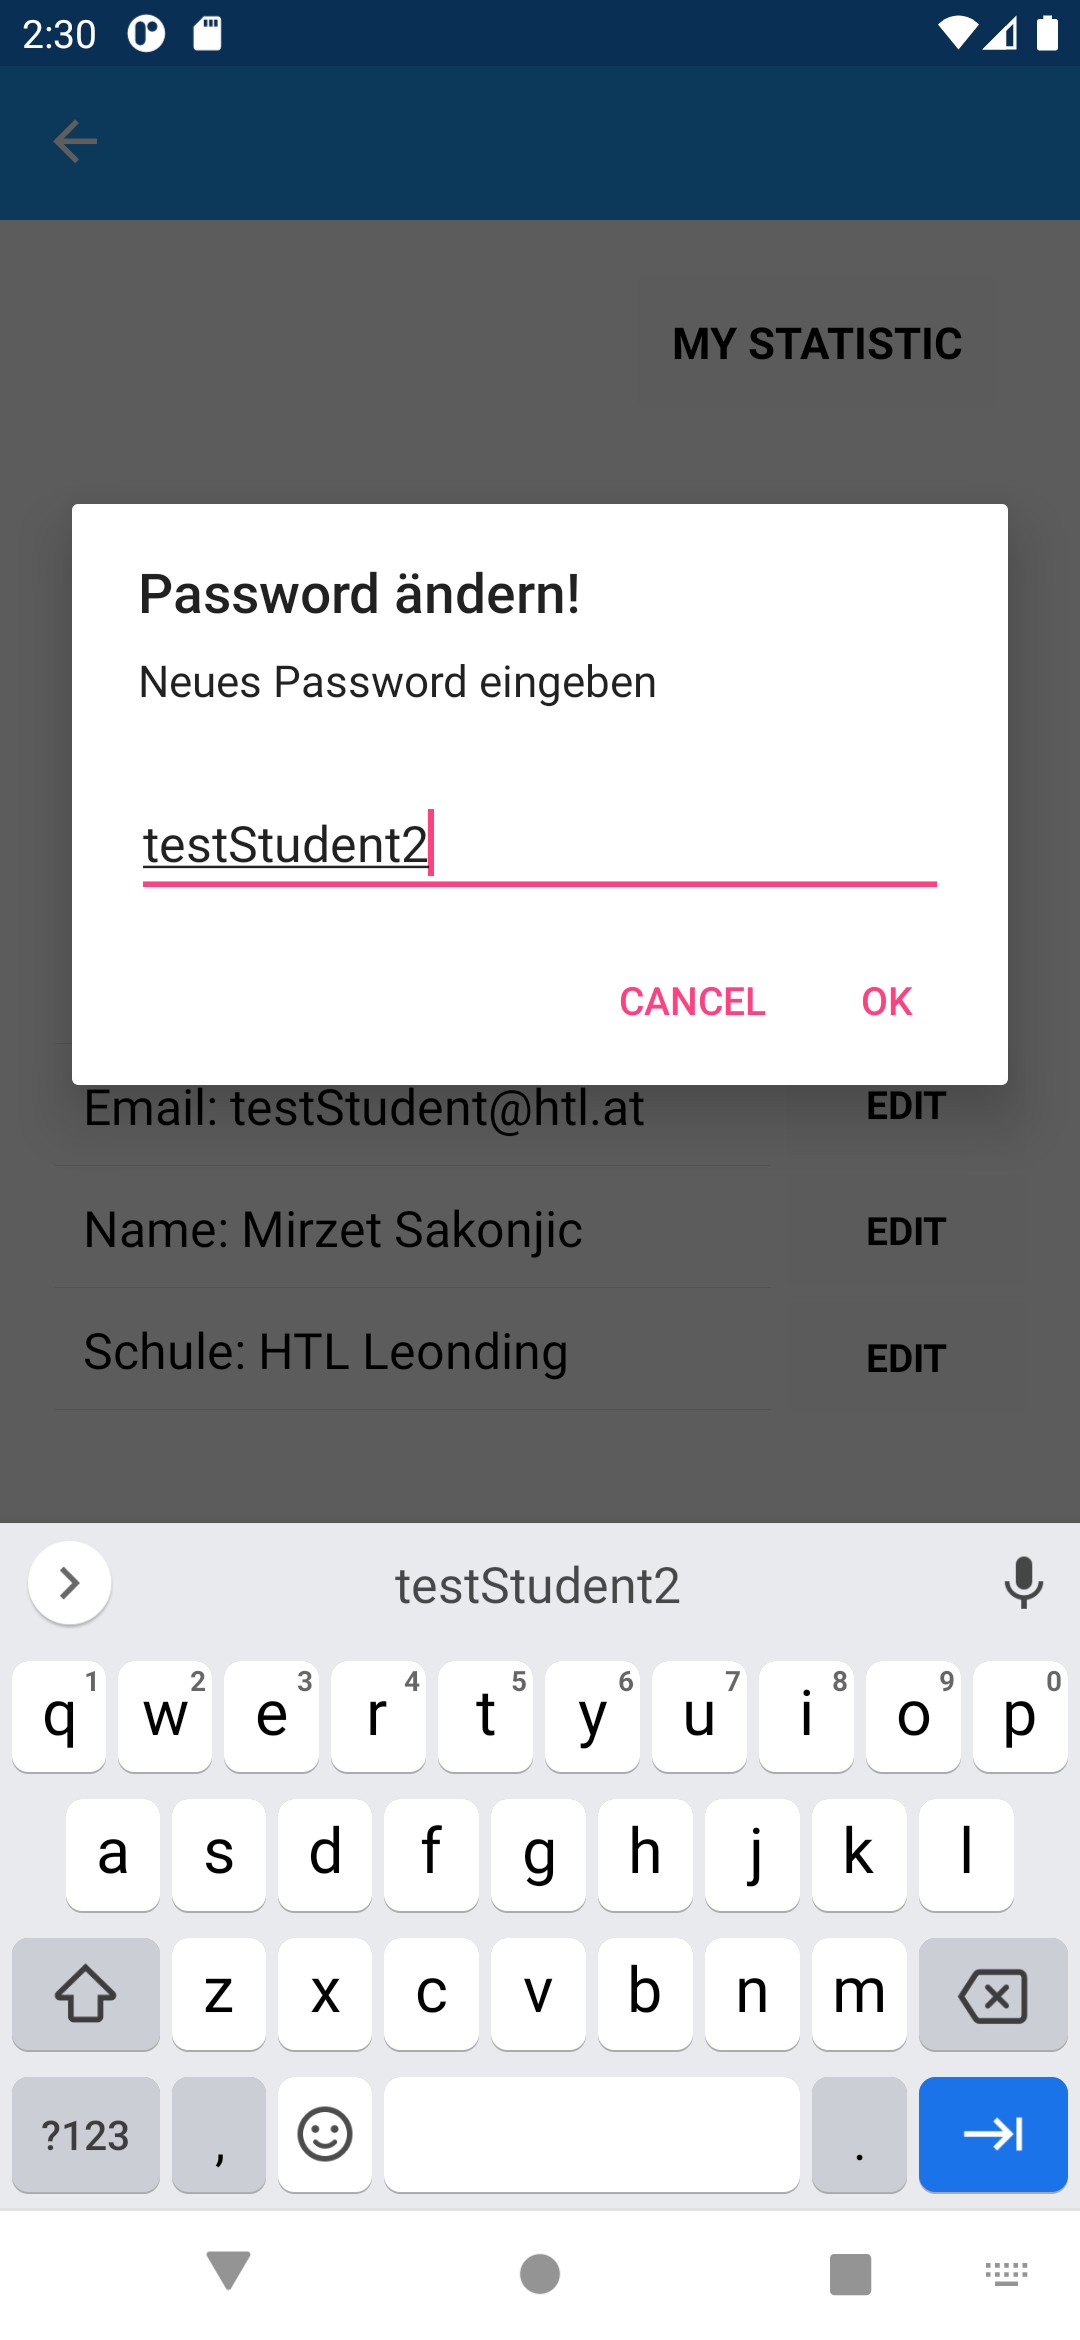
\includegraphics[width=5cm]{pics/Xamarin Student/21.png}\hfill
    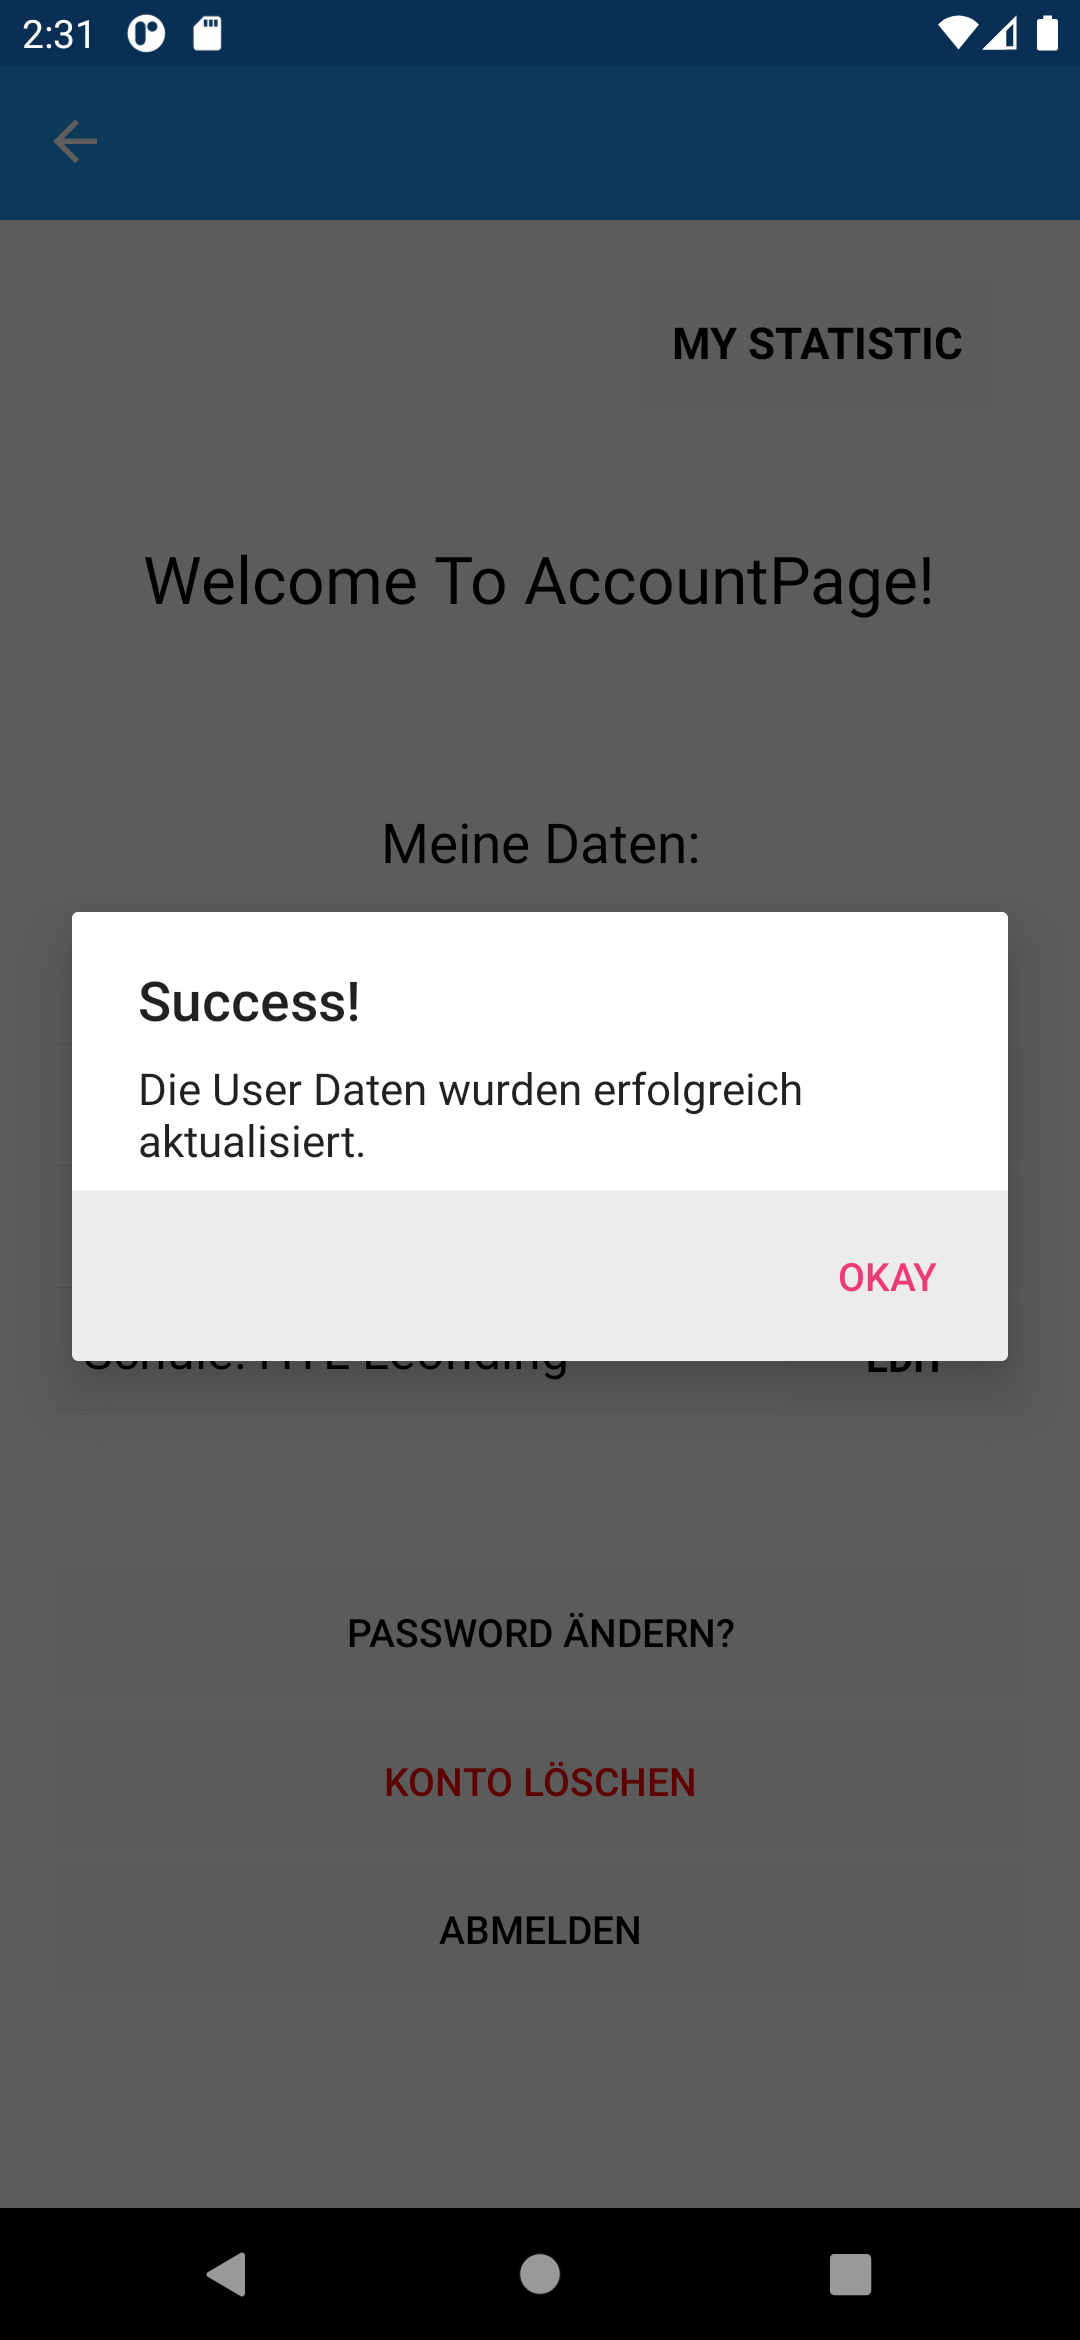
\includegraphics[width=5cm]{pics/Xamarin Student/22.png}
    \caption[MyAccount Passwort]{Passwort ändern}
    \end{center}
\end{figure}
\newpage
Das Löschen des Kontos ist durch Eingabe eines Passworts möglich, und alle Kontodaten werden entfernt und gelöscht.
\begin{figure}[h]
    \begin{center}
        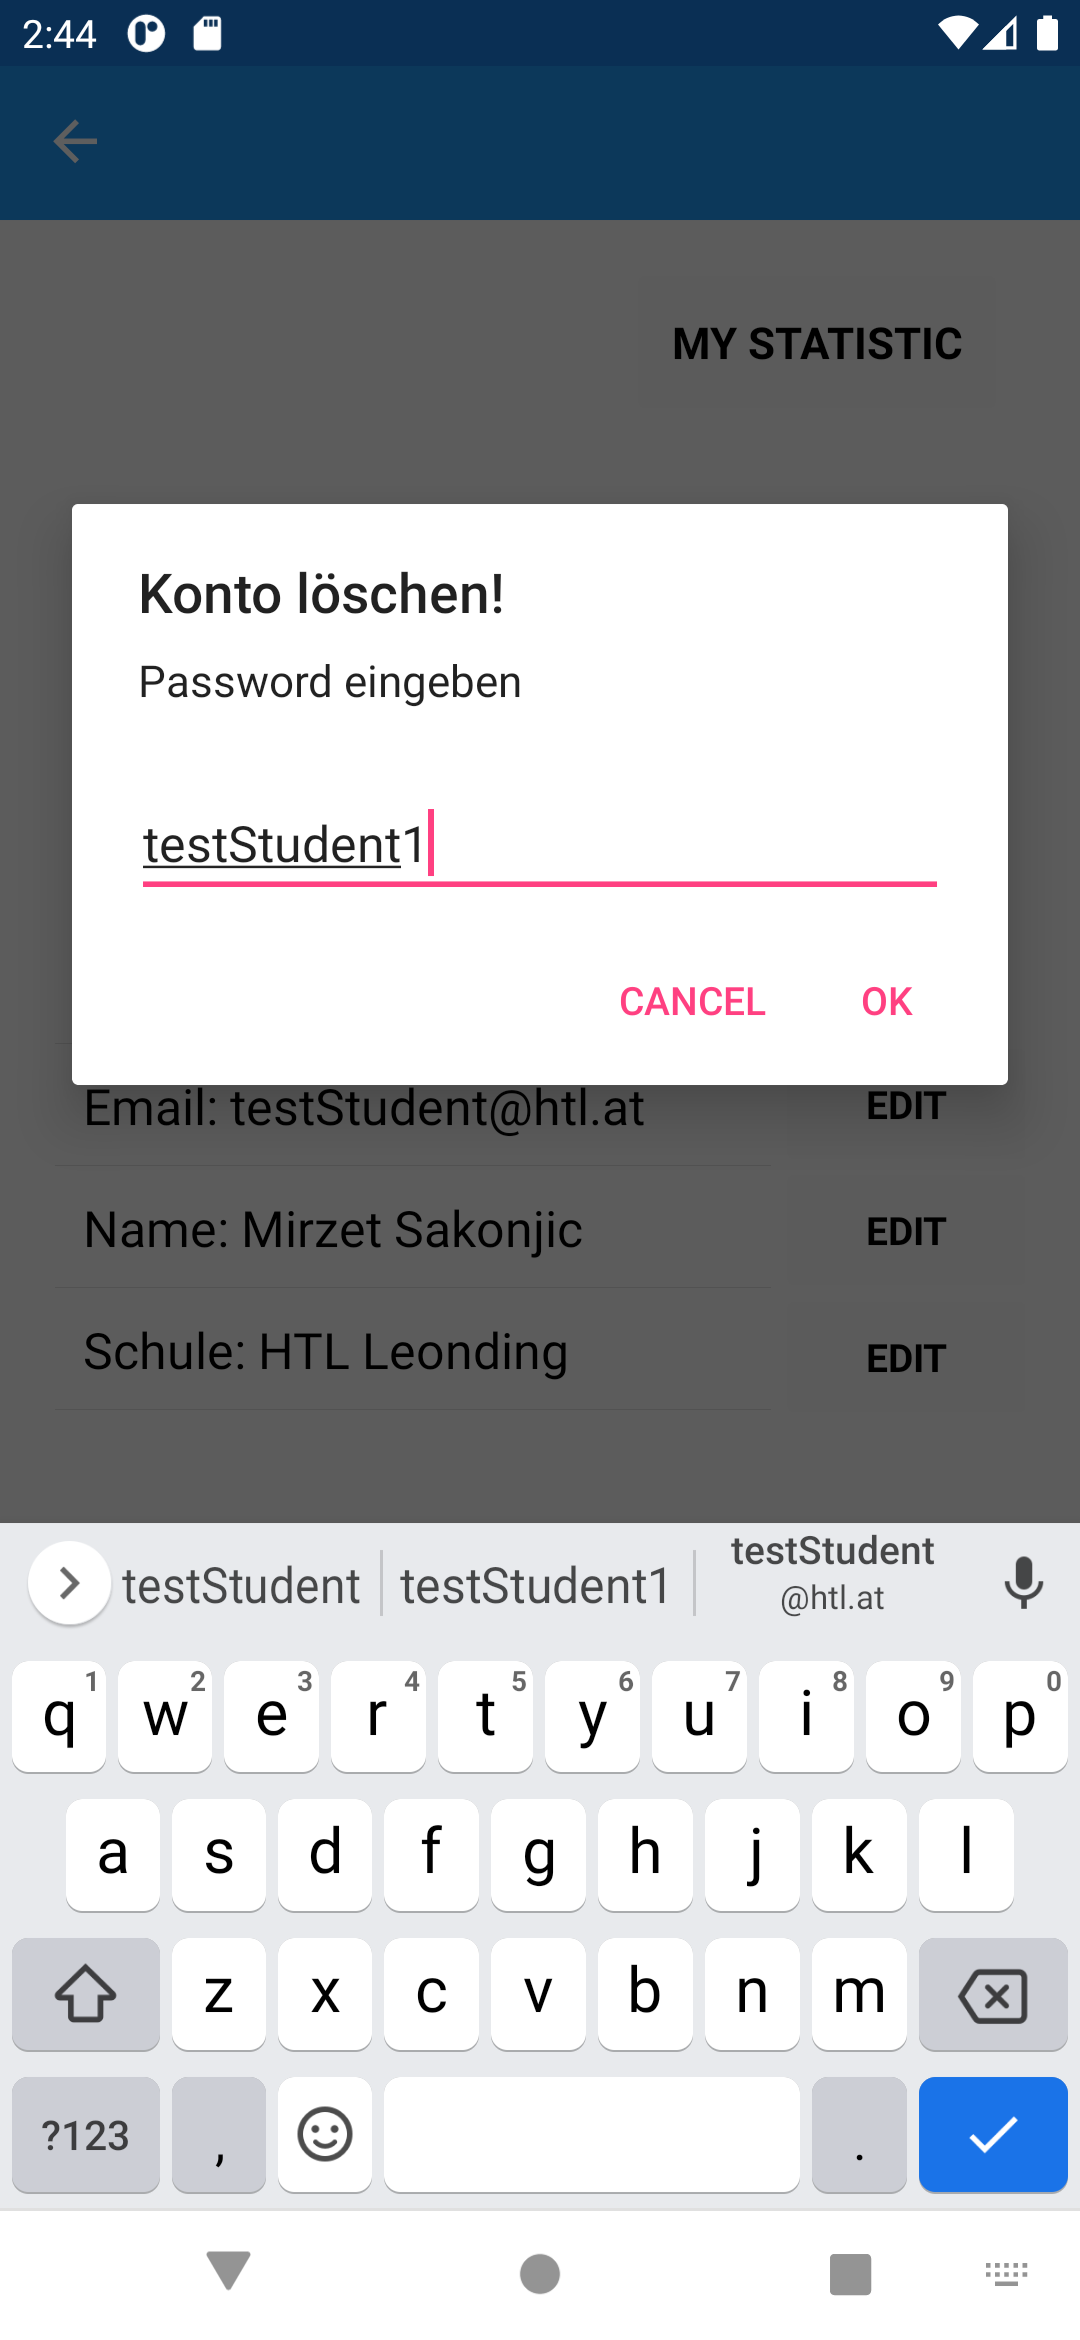
\includegraphics[width=5cm]{pics/Xamarin Student/25 Acc delete pass.png}\hfill
        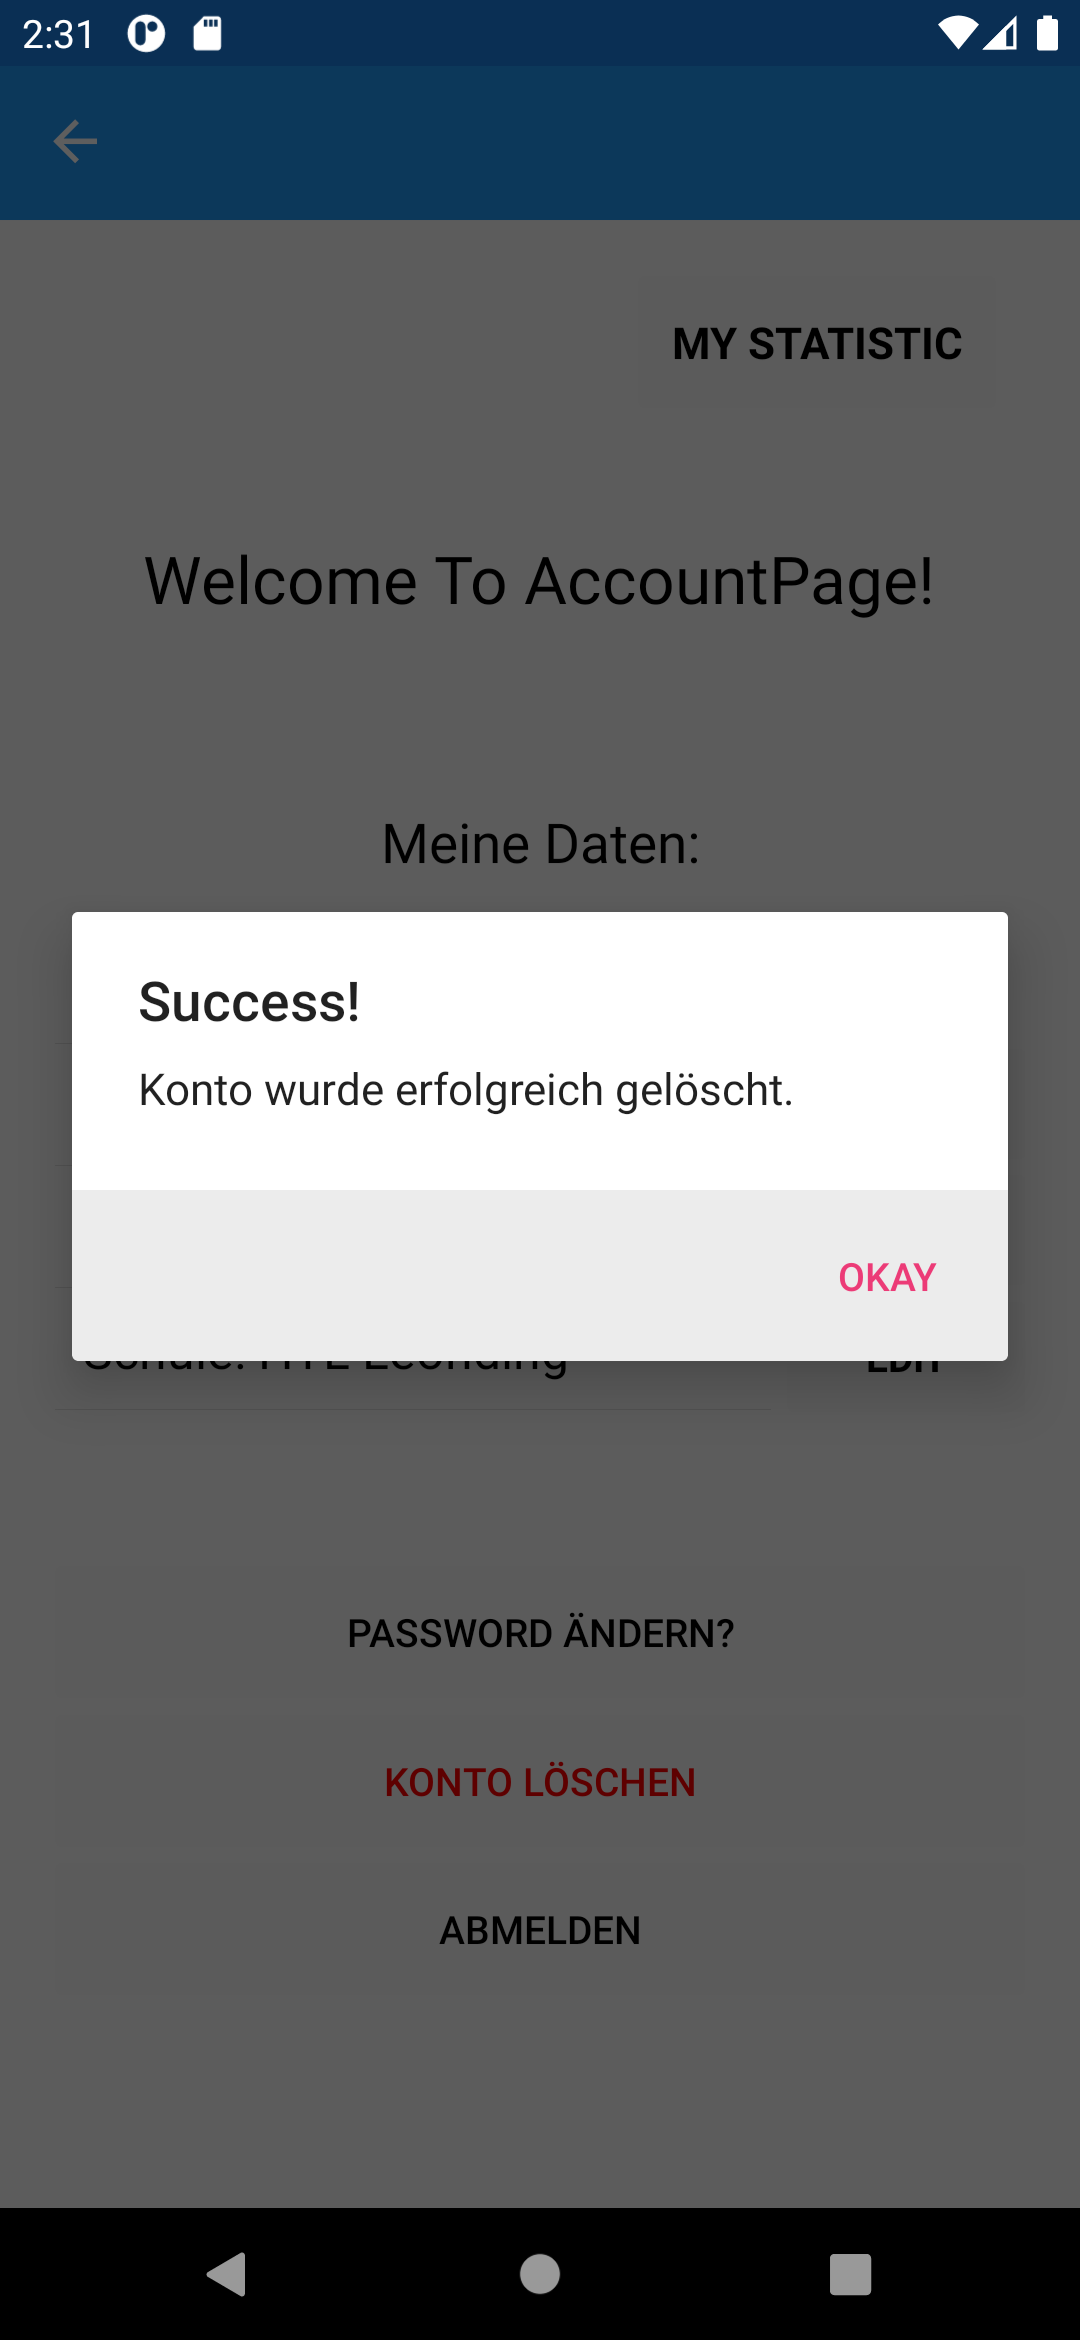
\includegraphics[width=5cm]{pics/Xamarin Student/23 Delete Acc.png}
        \end{center}
\end{figure}
\begin{figure}[h]
    \begin{center}
        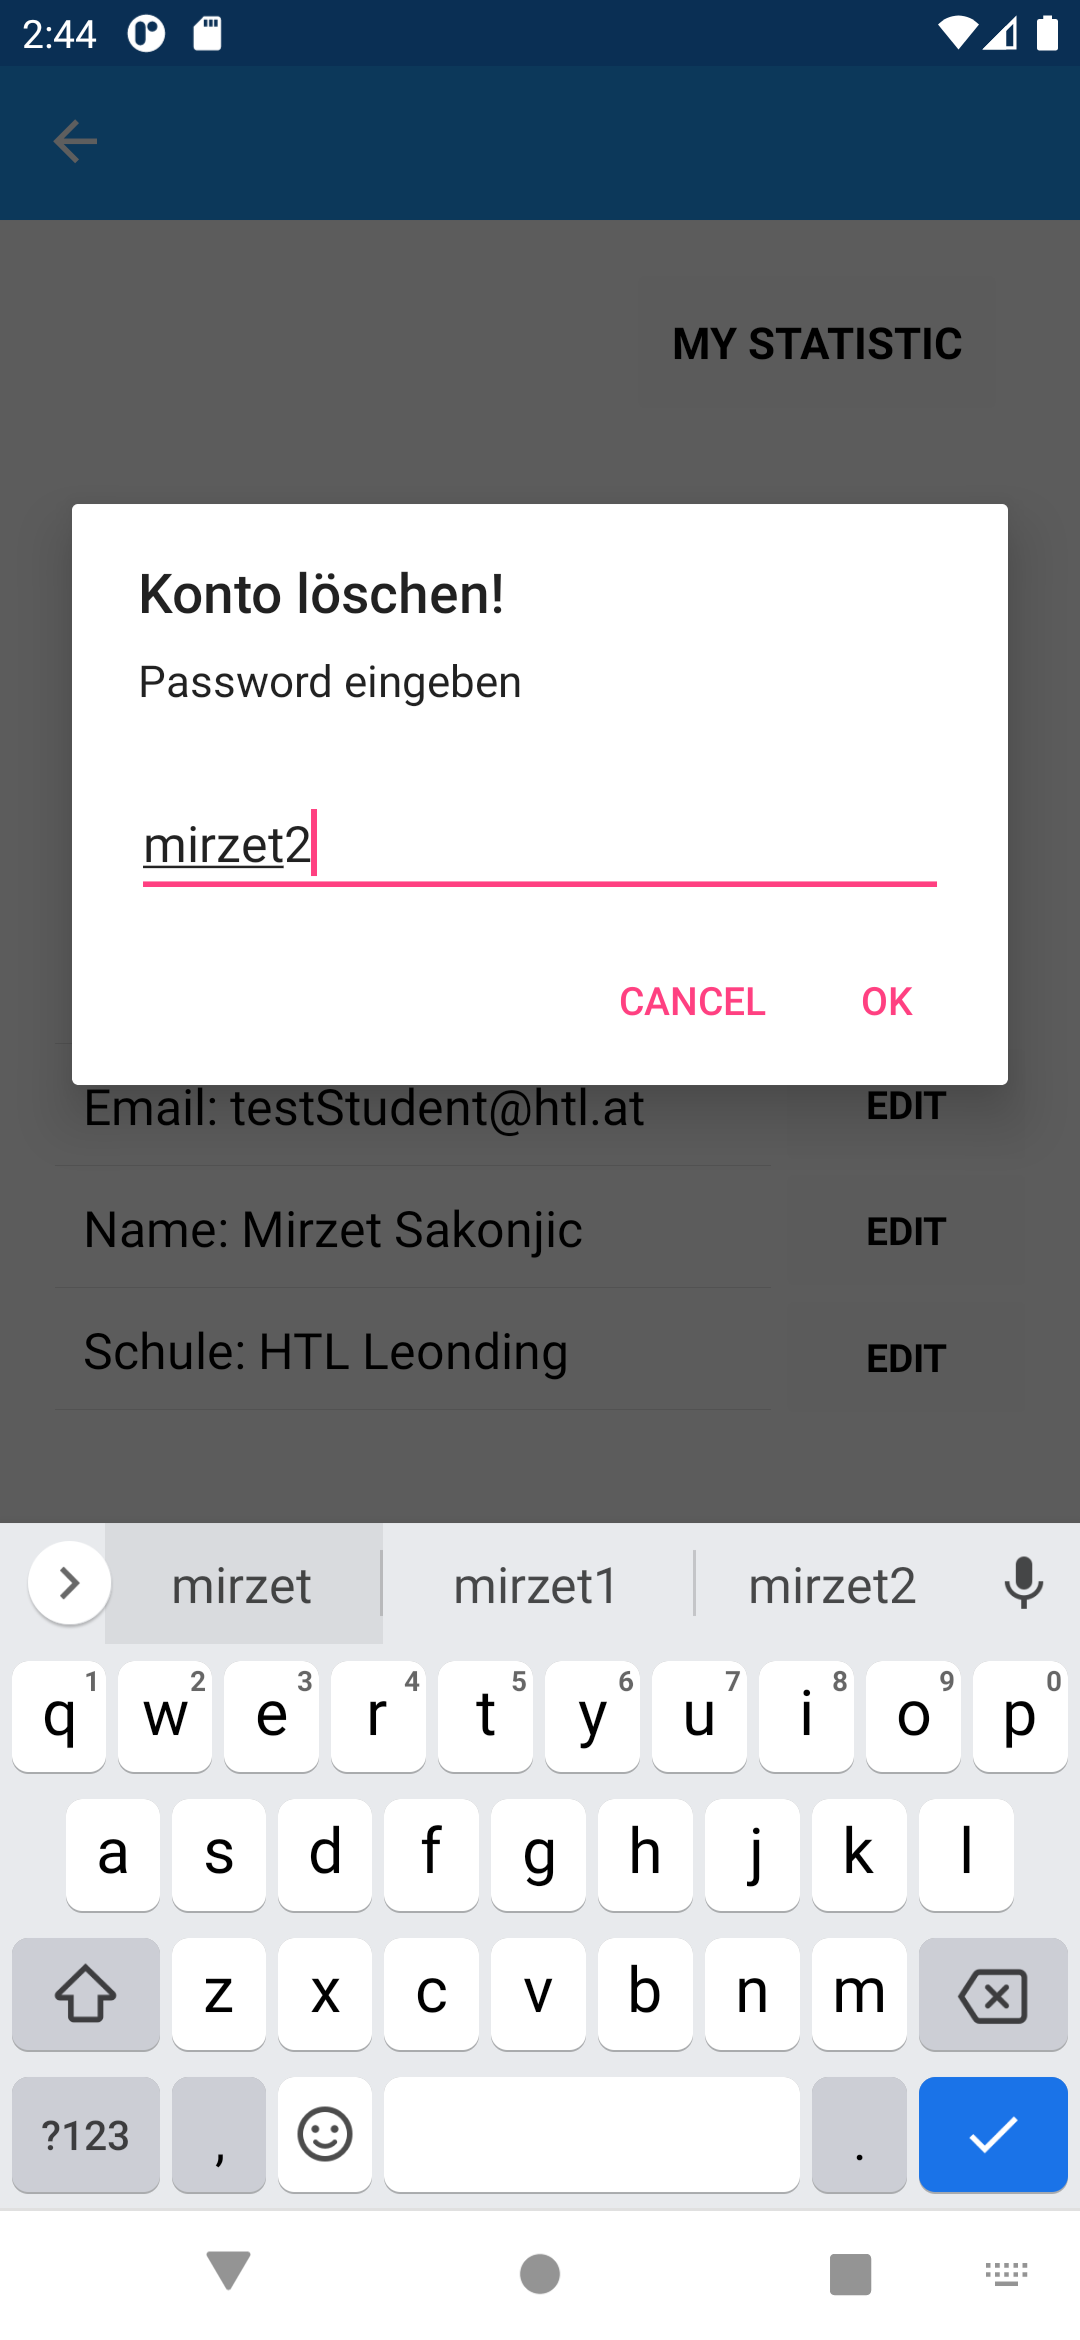
\includegraphics[width=5cm]{pics/Xamarin Student/23 Delete Acc Error.png}\hfill
        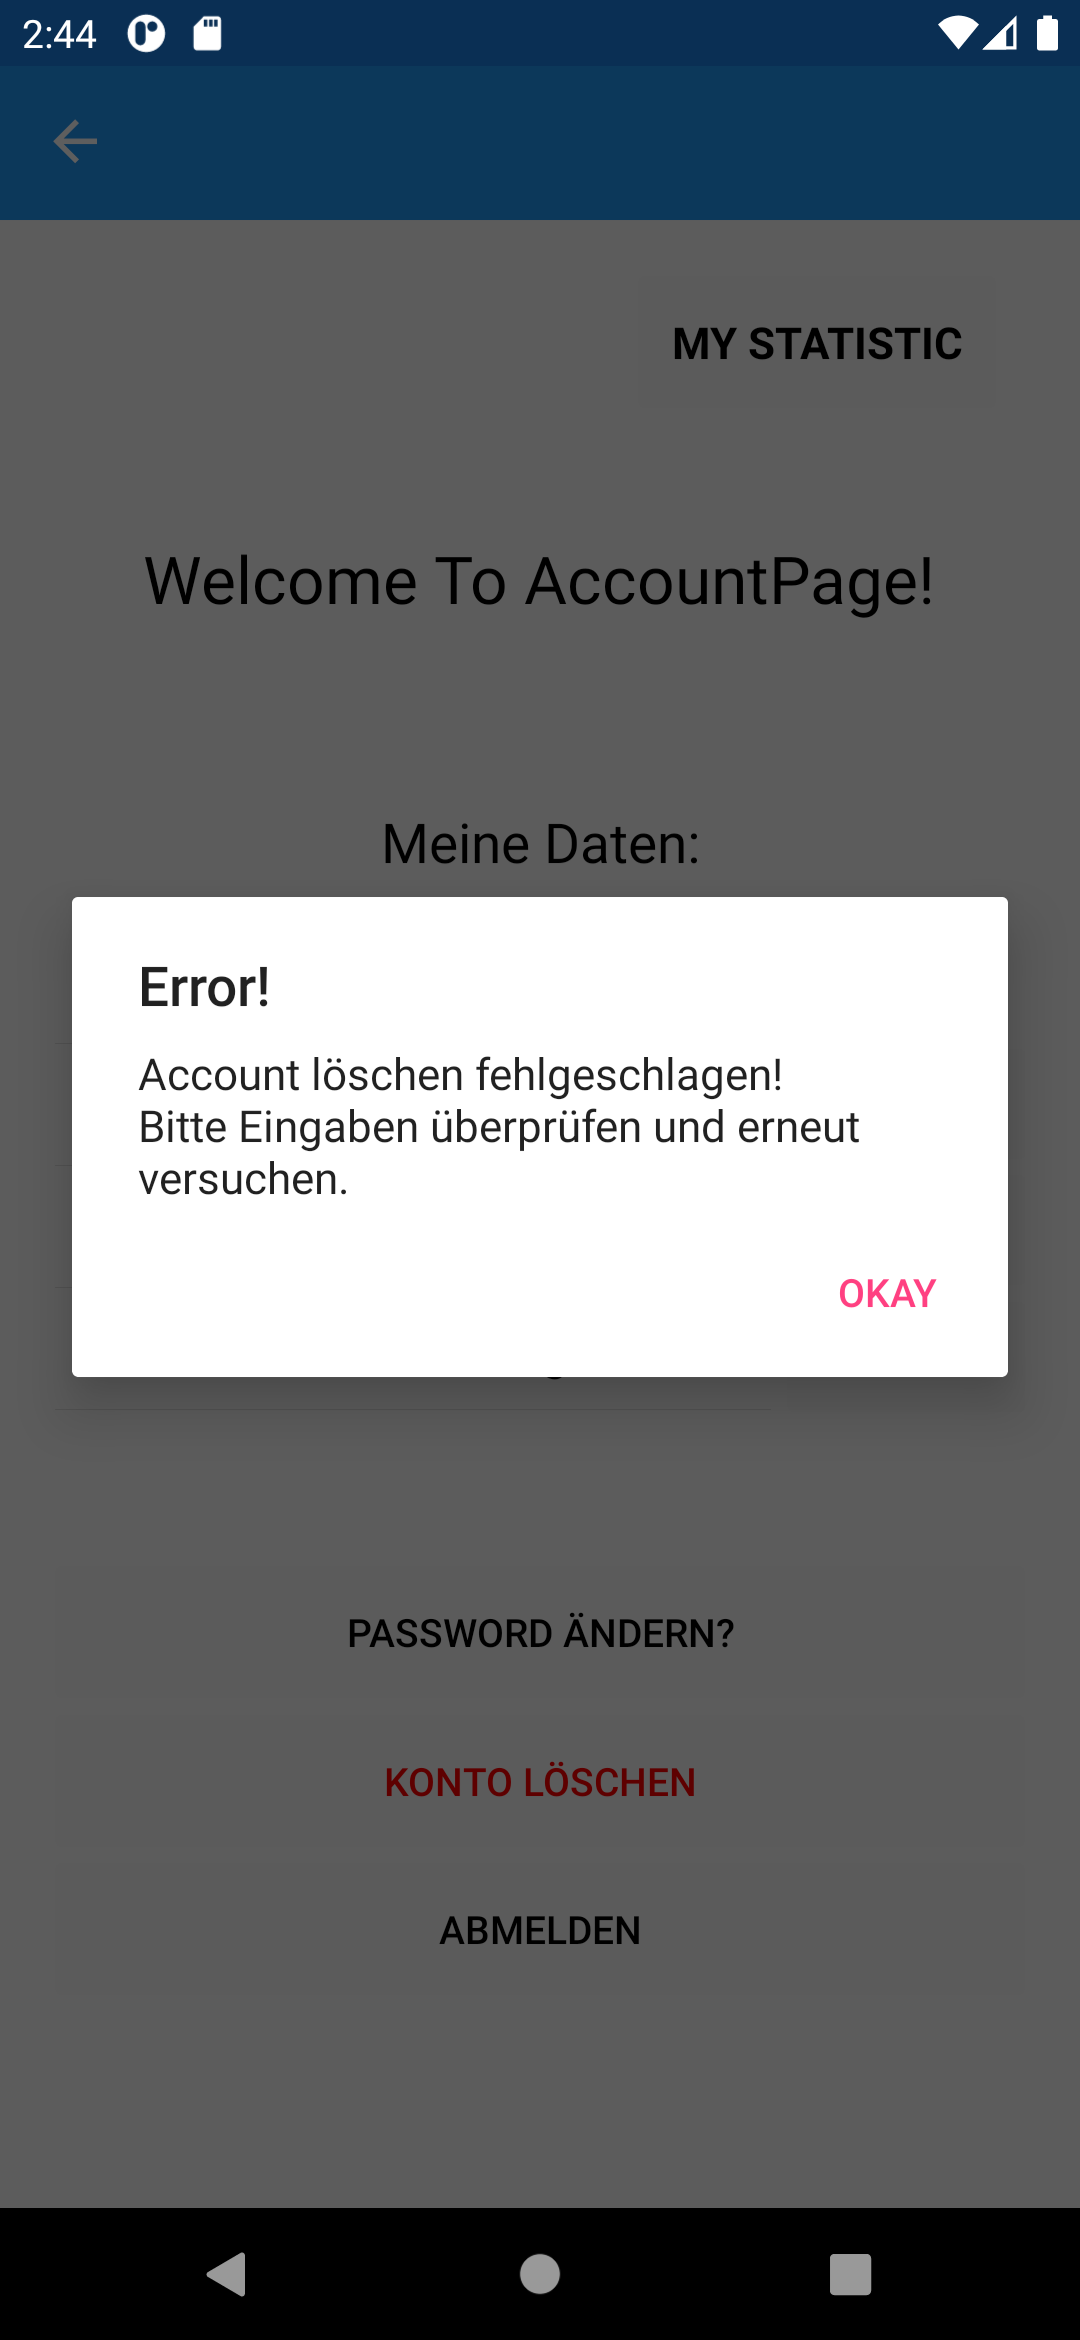
\includegraphics[width=5cm]{pics/Xamarin Student/24 Delete Acc Error.png}
        \caption[MyAccount Konto löschen]{Konto löschen}
        \end{center}
\end{figure}
Um sich abzumelden, müssen wir den Abmelden-Button drücken, und wir werden direkt auf die Login-Startseite zurückgeleitet.
Der einzige Unterschied auf der Benutzerkontoseite zwischen Schülern und Lehrern ist die Statistik in Button. So zeigt es für jeden Benutzer unterschiedliche Statistiken, zB wie viele Fächer der Lehrer eingegeben hat oder wie viel Feedback der Schüler gegeben hat.
\newpage

\section{Statistiken}
\subsection{Schüler}
Die Studentenstatistik wird in die Menge und Anzahl der abgegebenen Feedbacks eingerechnet. Das Messgerät zählt also alle Rückmeldungen und wirft eine Zahl als Summe aus.
\begin{figure}[h]
    \begin{center}
        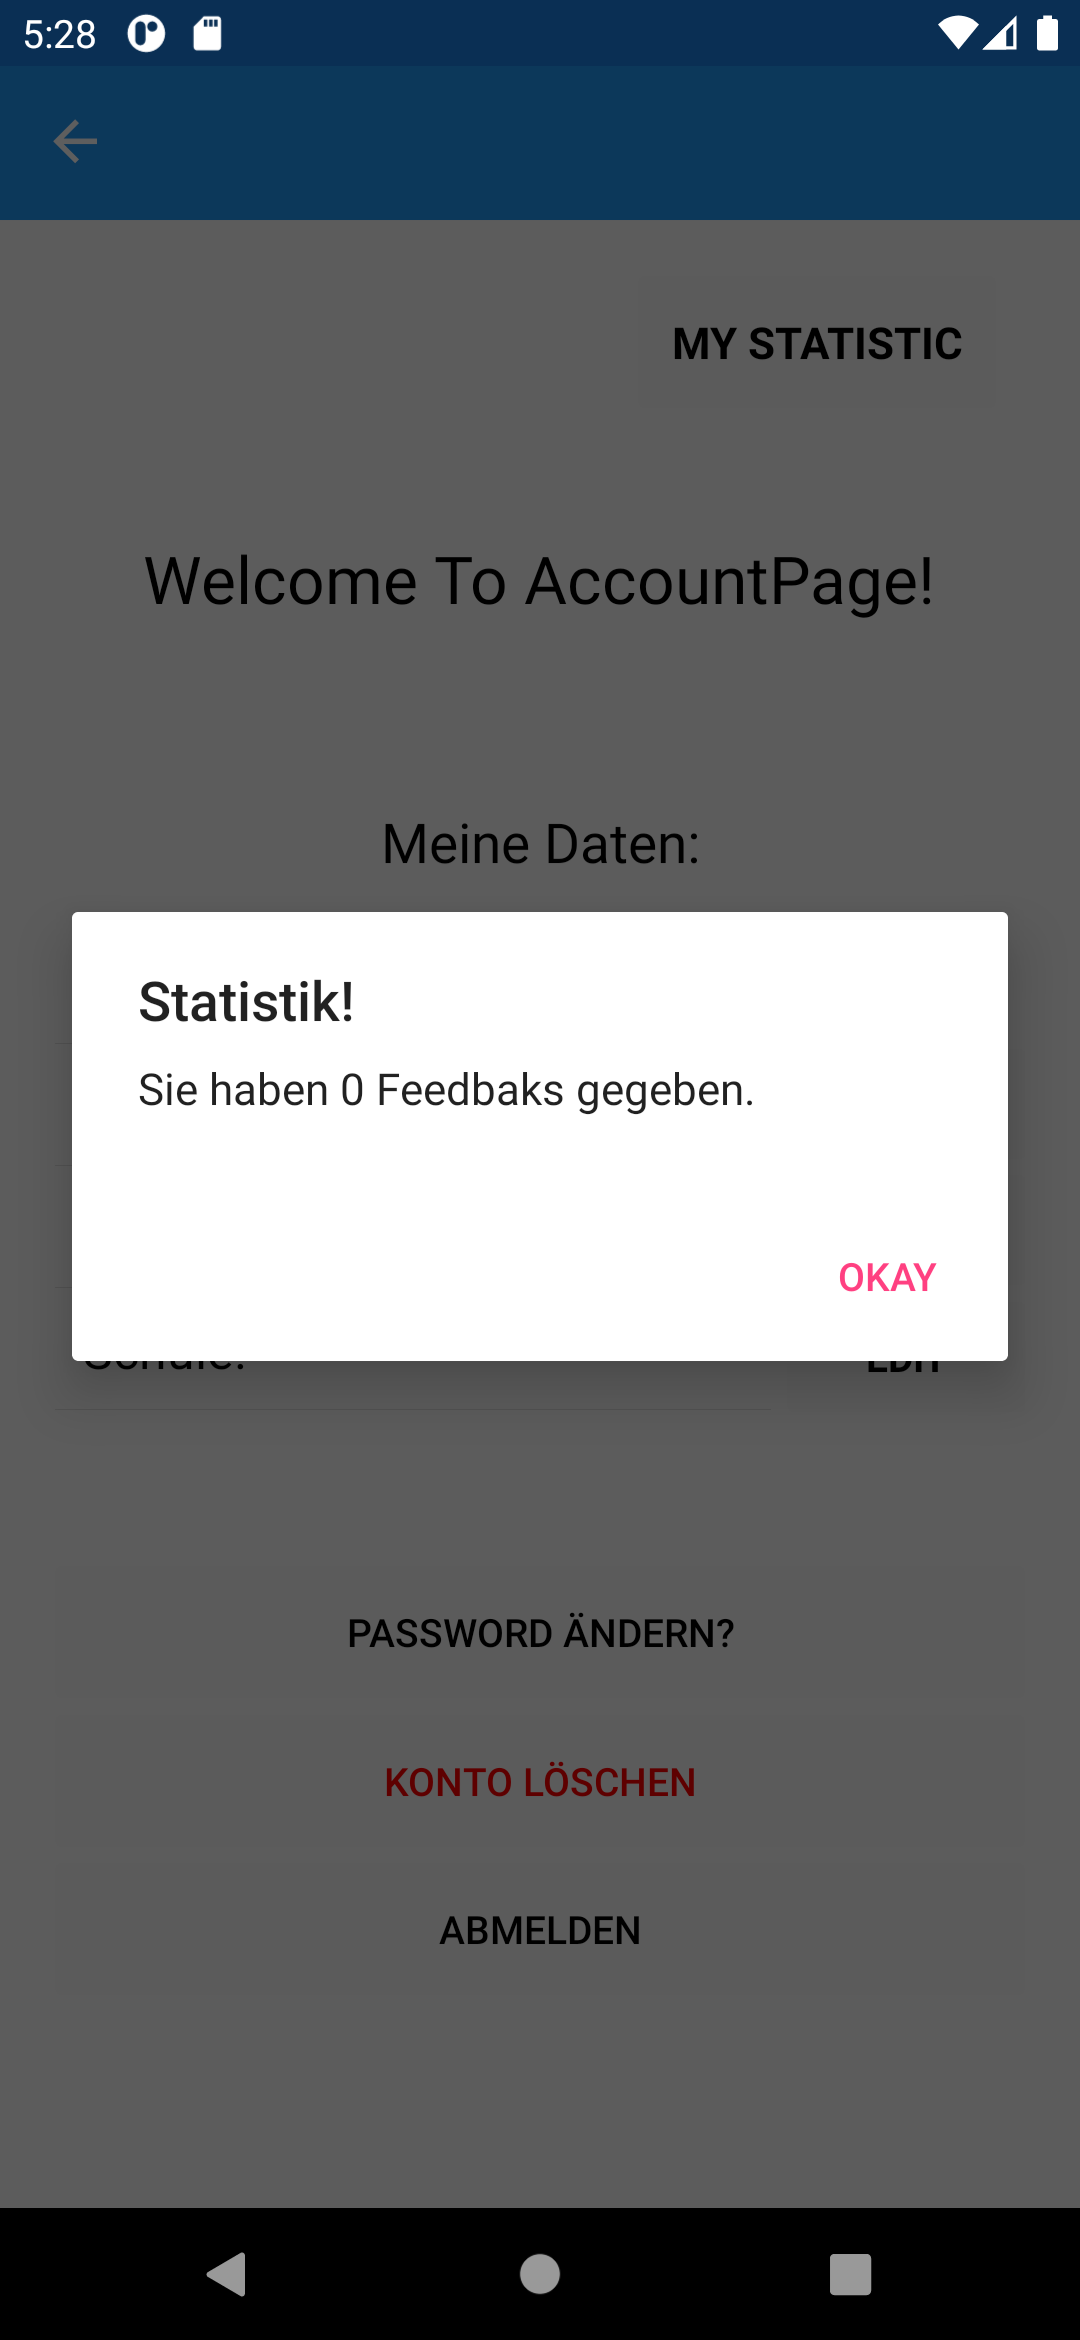
\includegraphics[width=5cm]{pics/Xamarin Student/27 Stat.png}\hfill
        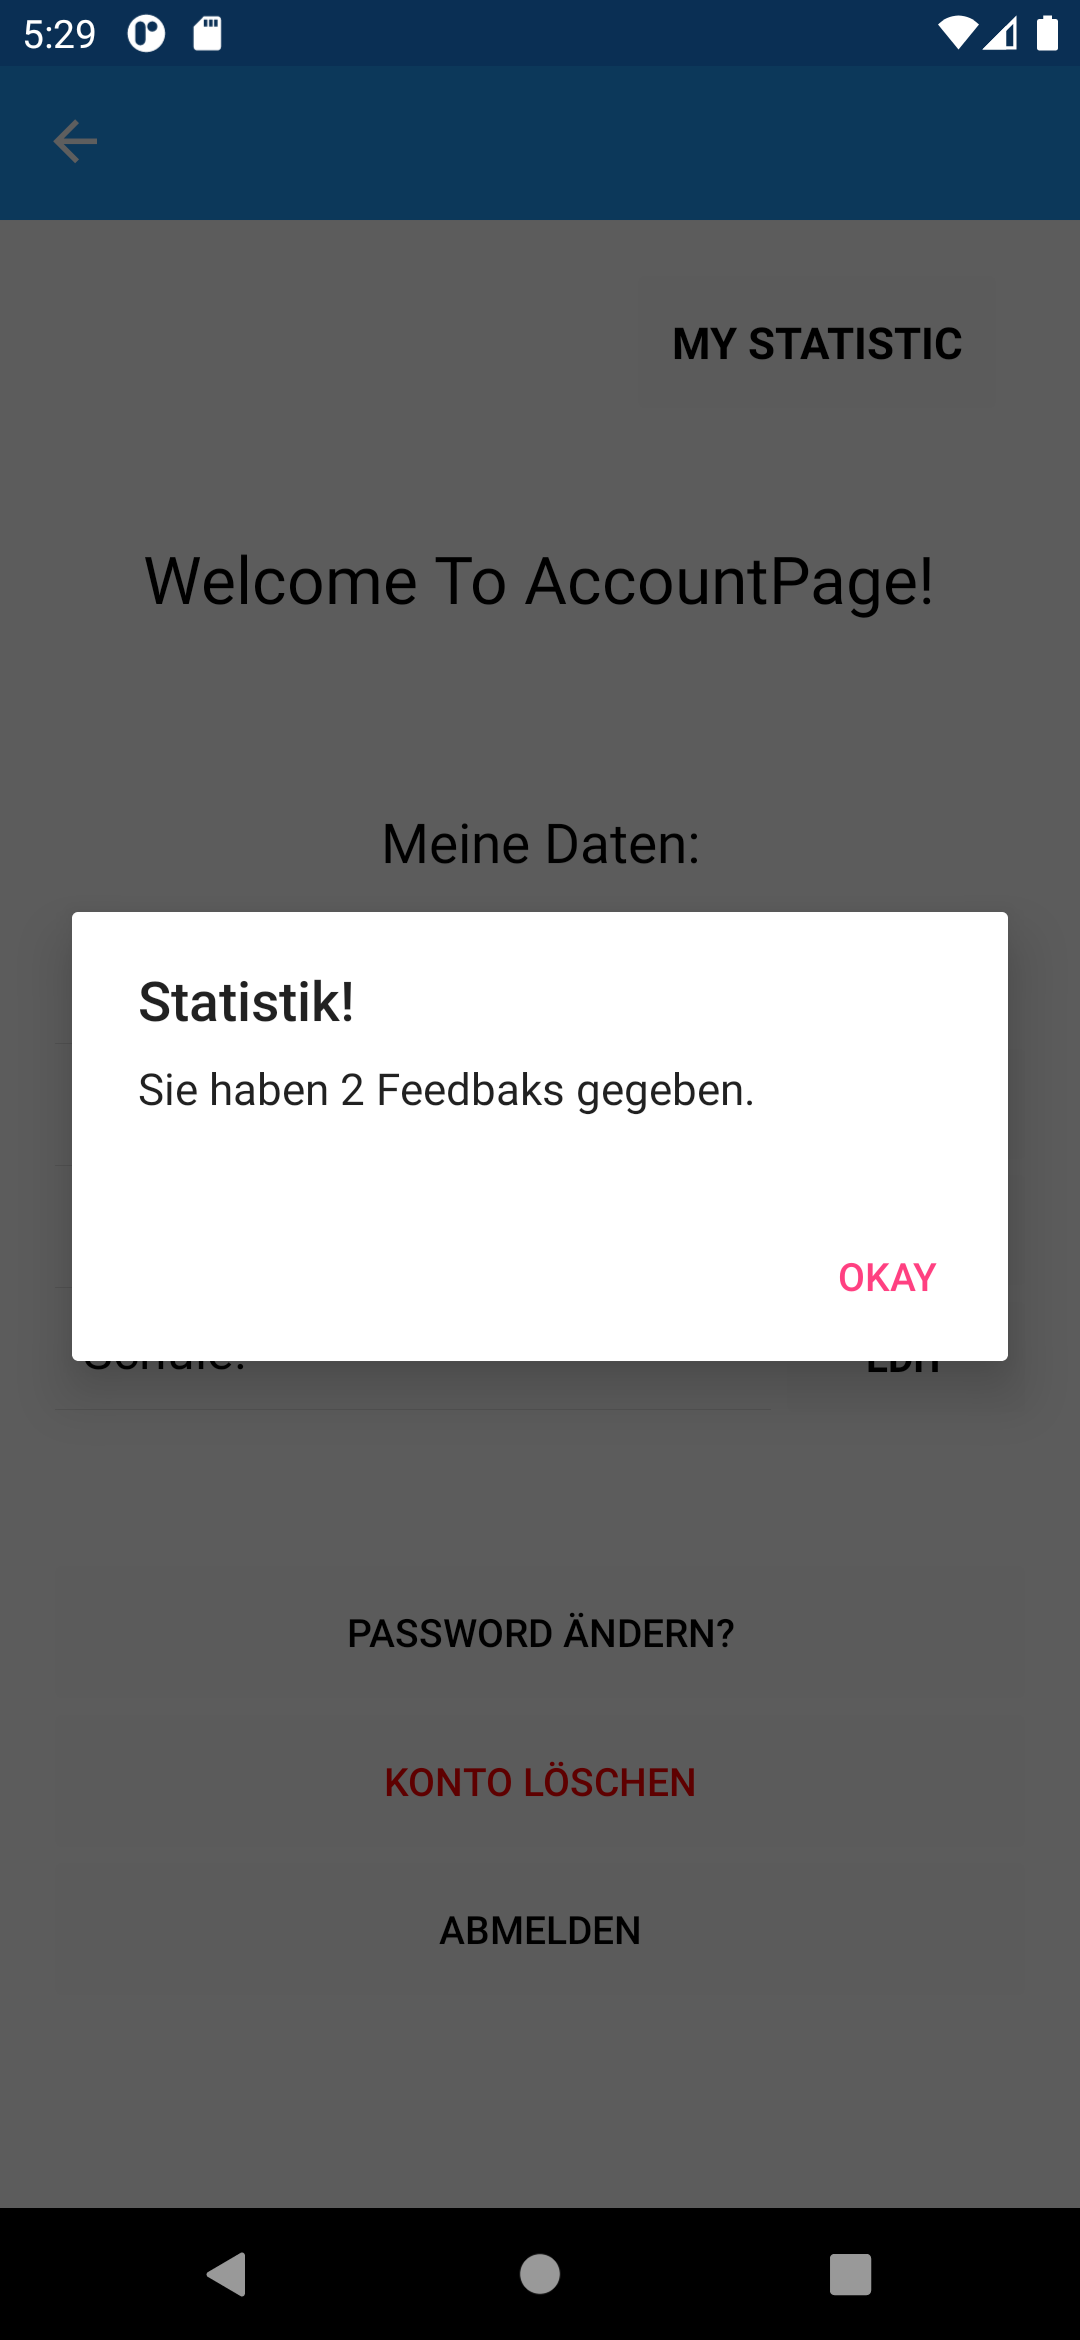
\includegraphics[width=5cm]{pics/Xamarin Student/28 Stat.png}
        \caption[Statistiken Schüler Ansicht]{Statistiken Schüler}
        \end{center}
\end{figure}
\newpage
\subsection{Lehrer}
Die Lehrerstatistik wird in der Menge und Anzahl der abgegebenen Feedbacks gezählt. Es zeigt zusätzlich die durchschnittliche Bewertung aller Feddbacks (AVG).
\begin{figure}[h]
    \begin{center}
        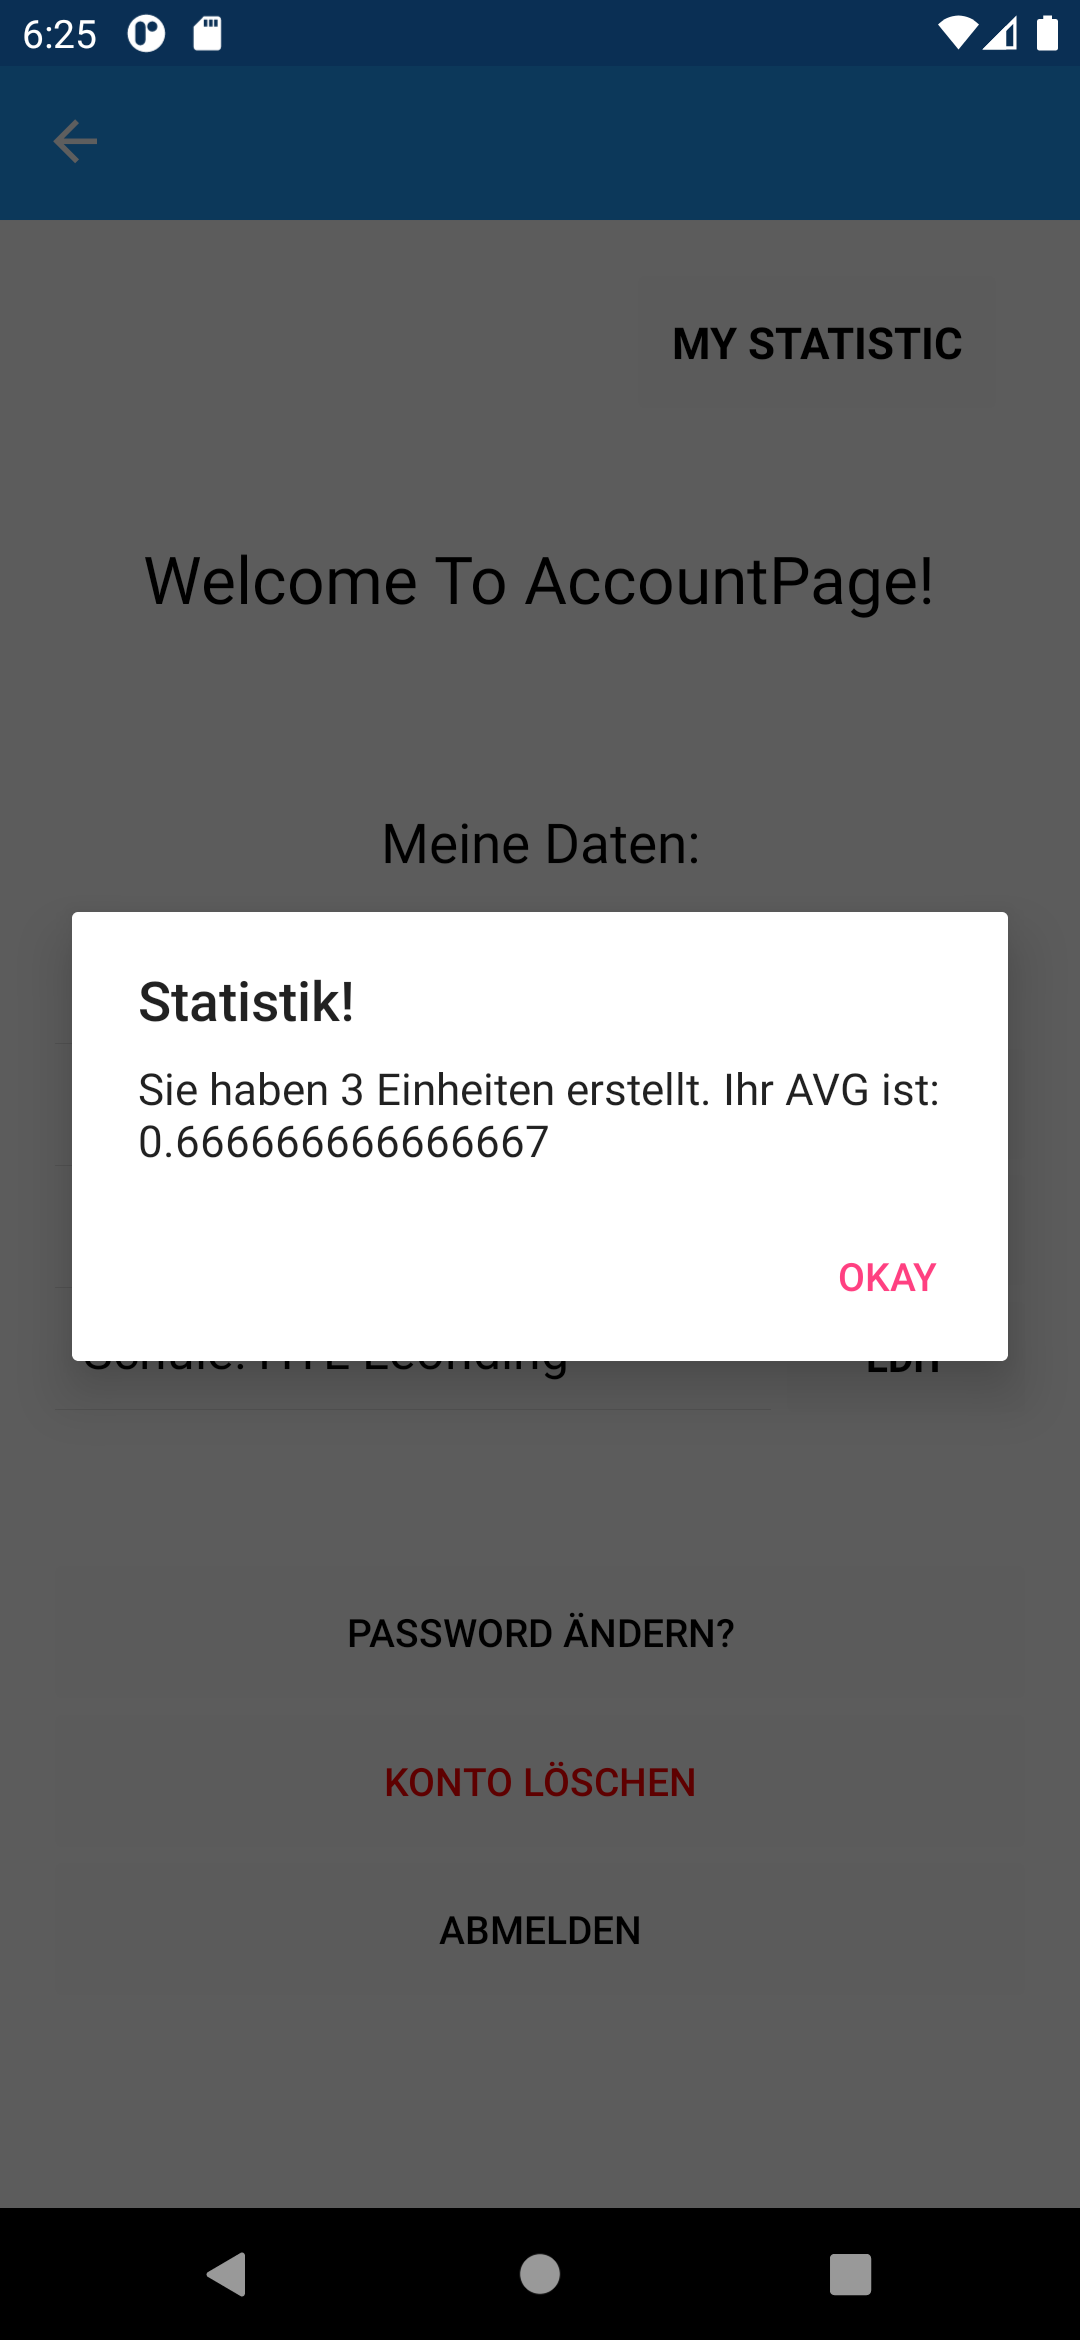
\includegraphics[width=5cm]{pics/Xamarin Lehrer/1 Stat.png}\hfill
        \caption[Statistiken Lehrer Ansicht]{Statistiken Lehrer}
        \end{center}
\end{figure}
\newpage